\documentclass[compress]{beamer}
\mode<presentation>
\setbeamercovered{transparent}
\usetheme{Warsaw}
%\useoutertheme{smoothtree}
\usepackage{multirow}
\usepackage[english]{babel}
\usepackage[latin1]{inputenc}
\usepackage{times}
\usepackage[T1]{fontenc}
\usepackage{xmpmulti}
\usepackage{multicol}
\usepackage{colortbl}

%\setbeamersize{text margin left=.25 in,text margin right=.25 in}
\setbeamersize{text margin left=.15 in,text margin right=.15 in}
\usepackage[authoryear]{natbib}


\usepackage{epstopdf}
\usepackage{xcolor}
\usepackage{latexcolors}
%\usepackage[dvipsnames]{xcolor}
\definecolor{antiquebrass}{rgb}{0.8, 0.58, 0.46}
\definecolor{babyblueeyes}{rgb}{0.63, 0.79, 0.95}
\definecolor{babyblue}{rgb}{0.54, 0.81, 0.94}
\definecolor{bistre}{rgb}{0.24, 0.17, 0.12}
\definecolor{brightlavender}{rgb}{0.75, 0.58, 0.89}
\definecolor{bulgarianrose}{rgb}{0.28, 0.02, 0.03}
%\definecolor{slateblue}{rgb}{0.56, 0.74, 0.56}
\definecolor{cordovan}{rgb}{0.54, 0.25, 0.27}
\definecolor{darkbyzantium}{rgb}{0.36, 0.22, 0.33}

\setbeamercolor{structure}{fg=atomictangerine!90, bg= black!60}







\usepackage{tikz}
\usetikzlibrary{shadows,calc}
\usetikzlibrary{shadows.blur}
\usetikzlibrary{shapes.symbols}
\usepackage{hyperref}
\usepackage{booktabs}
\usepackage{colortbl}
\usepackage{multirow}
%%%%%%%%% shaddow image %%%%%
% some parameters for customization
\def\shadowshift{3pt,-3pt}
\def\shadowradius{6pt}
\colorlet{innercolor}{black!60}
\colorlet{outercolor}{gray!05}
% this draws a shadow under a rectangle node
\newcommand\drawshadow[1]{
\begin{pgfonlayer}{shadow}
    \shade[outercolor,inner color=innercolor,outer color=outercolor] ($(#1.south west)+(\shadowshift)+(\shadowradius/2,\shadowradius/2)$) circle (\shadowradius);
    \shade[outercolor,inner color=innercolor,outer color=outercolor] ($(#1.north west)+(\shadowshift)+(\shadowradius/2,-\shadowradius/2)$) circle (\shadowradius);
    \shade[outercolor,inner color=innercolor,outer color=outercolor] ($(#1.south east)+(\shadowshift)+(-\shadowradius/2,\shadowradius/2)$) circle (\shadowradius);
    \shade[outercolor,inner color=innercolor,outer color=outercolor] ($(#1.north east)+(\shadowshift)+(-\shadowradius/2,-\shadowradius/2)$) circle (\shadowradius);
    \shade[top color=innercolor,bottom color=outercolor] ($(#1.south west)+(\shadowshift)+(\shadowradius/2,-\shadowradius/2)$) rectangle ($(#1.south east)+(\shadowshift)+(-\shadowradius/2,\shadowradius/2)$);
    \shade[left color=innercolor,right color=outercolor] ($(#1.south east)+(\shadowshift)+(-\shadowradius/2,\shadowradius/2)$) rectangle ($(#1.north east)+(\shadowshift)+(\shadowradius/2,-\shadowradius/2)$);
    \shade[bottom color=innercolor,top color=outercolor] ($(#1.north west)+(\shadowshift)+(\shadowradius/2,-\shadowradius/2)$) rectangle ($(#1.north east)+(\shadowshift)+(-\shadowradius/2,\shadowradius/2)$);
    \shade[outercolor,right color=innercolor,left color=outercolor] ($(#1.south west)+(\shadowshift)+(-\shadowradius/2,\shadowradius/2)$) rectangle ($(#1.north west)+(\shadowshift)+(\shadowradius/2,-\shadowradius/2)$);
    \shade[outercolor,right color=innercolor,left color=innercolor] ($(#1.north west)+(-\shadowradius/12,\shadowradius/12)$) rectangle ($(#1.south east)+(\shadowradius/12,-\shadowradius/12)$);%Frame
    \filldraw ($(#1.south west)+(\shadowshift)+(\shadowradius/2,\shadowradius/2)$) rectangle ($(#1.north east)+(\shadowshift)-(\shadowradius/2,\shadowradius/2)$);
\end{pgfonlayer}
}
% create a shadow layer, so that we don't need to worry about overdrawing other things
\pgfdeclarelayer{shadow} 
\pgfsetlayers{shadow,main}
% Define image shadow command
\newcommand\shadowimage[2][]{%
\begin{tikzpicture}
\node[anchor=south west,inner sep=0] (image) at (0,0) {\includegraphics[#1]{#2}};
\drawshadow{image}
\end{tikzpicture}}
\usepackage{calligra}

\DeclareMathOperator*{\argmax}{Arg\,max}
\DeclareMathOperator*{\argmin}{Arg\,min}
\newcommand{\norm}[1]{\left\Vert #1 \right\Vert }
\newcommand{\bbetaHat}{ \widehat{\bbeta}}
\newcommand{\bbetaLSE}{ \widehat{\bbeta}_{_{\text{LSE}}}}
\newcommand{\bbetaMLE}{ \widehat{\bbeta}_{_{\text{MLE}}}}
\newcommand{\sqBullet}[1]{  {\tiny \tiny \tiny \qBoxCol{#1!60}{ }} }
%***************
%\newtheorem{thm}{Theorem}
\input{definition_include.tex}
\input{BoxDef}
\input{MatrixDef}











\title{  STAT 380:\\ {\color{black}  Ensemble Methods: Random Forest \& Boosting  }}

\author[UAEU]
{UAEU}
\institute[UAEU] % (optional, but mostly needed)
{
  \inst{}%
  %Indian Institute of Management,  Udaipur\\
  \vspace{0.1in}

  
}

\date{}


\newcommand{\Xnew}{ \HLTEQ[orange]{X_{_{\text{i}}}} }
\newcommand{\Ynew}{ \HLTEQ[orange]{Y_{_{\text{i}}}} }

%\date{\today}

\AtBeginSection[]
{
  \begin{frame}{Inhalt}
 % \begin{multicols}{1}
	\frametitle{Outline}
    \tableofcontents[currentsection]
  %  \end{multicols}
  \end{frame}
}

\begin{document}
\maketitle





\begin{frame}{Outlook of the unit}
	
	\begin{itemize}
		\item \textbf{Bagging}
		\item \textbf{Random Forest}
		\item \textbf{Boosting}
		\end{itemize}		
\end{frame}


%\TransitionFrame[antiquebrass]{\Large  Evaluating  Performance of a Classification Technique}
%
%\begin{frame}
%	\frametitle{ }
%	\begin{itemize}
%\item[ ] \qbx[4.1in]{purple!40}{\sqBullet{purple}A natural criterion for judging the performance of a classifier is the probability
%of making a \textbf{misclassification} error.}
%			\vspace{0.2cm}
%		\item[]  \qbx[4.1in]{teal!40}{ \sqBullet{teal}Misclassification means that the record
%belongs to one class but the model classifies it as a member of a different class.}
%			\vspace{0.2cm}
%		\item[ ] \qbx[4.1in]{apricot!40}{\sqBullet{brown} Is there a minimal
%probability of misclassification that we should require of a classifier?}
%	
%			\vspace{0.2cm}
%		\item[ ] \qbx[4.1in]{amber!40}{\sqBullet{amber} A classifier that makes no errors would be perfect - unrealistic.}
%	
%		
%	\end{itemize}
%\end{frame}


%
%
%\begin{frame}
%\qBrd[4.5in]{olive!30}{\sqBullet{olive}
%Let's consider a simple example to un derstand the working mechanism of  the regression trees. \\
%\qBrd[4.2in]{teal!30}{Suppose that we want to
%predict a baseball player's (log-scale) salary based on the following predictor
%variables: years (number of years in MLB) and hits (number of hits in previous
%year). }
%}
%\end{frame}


\section{Bagging}
\TransitionFrame[airforceblue]{\Large Bagging }


\begin{frame}\frametitle{ Standard Decision Tree may not be robust}
\qBrd[4.5in]{babyblue!50}{
\sqBullet{blue}
Three Entirely different Decision trees has been estimated based on three different sub samples of a Data set. 
\begin{center}
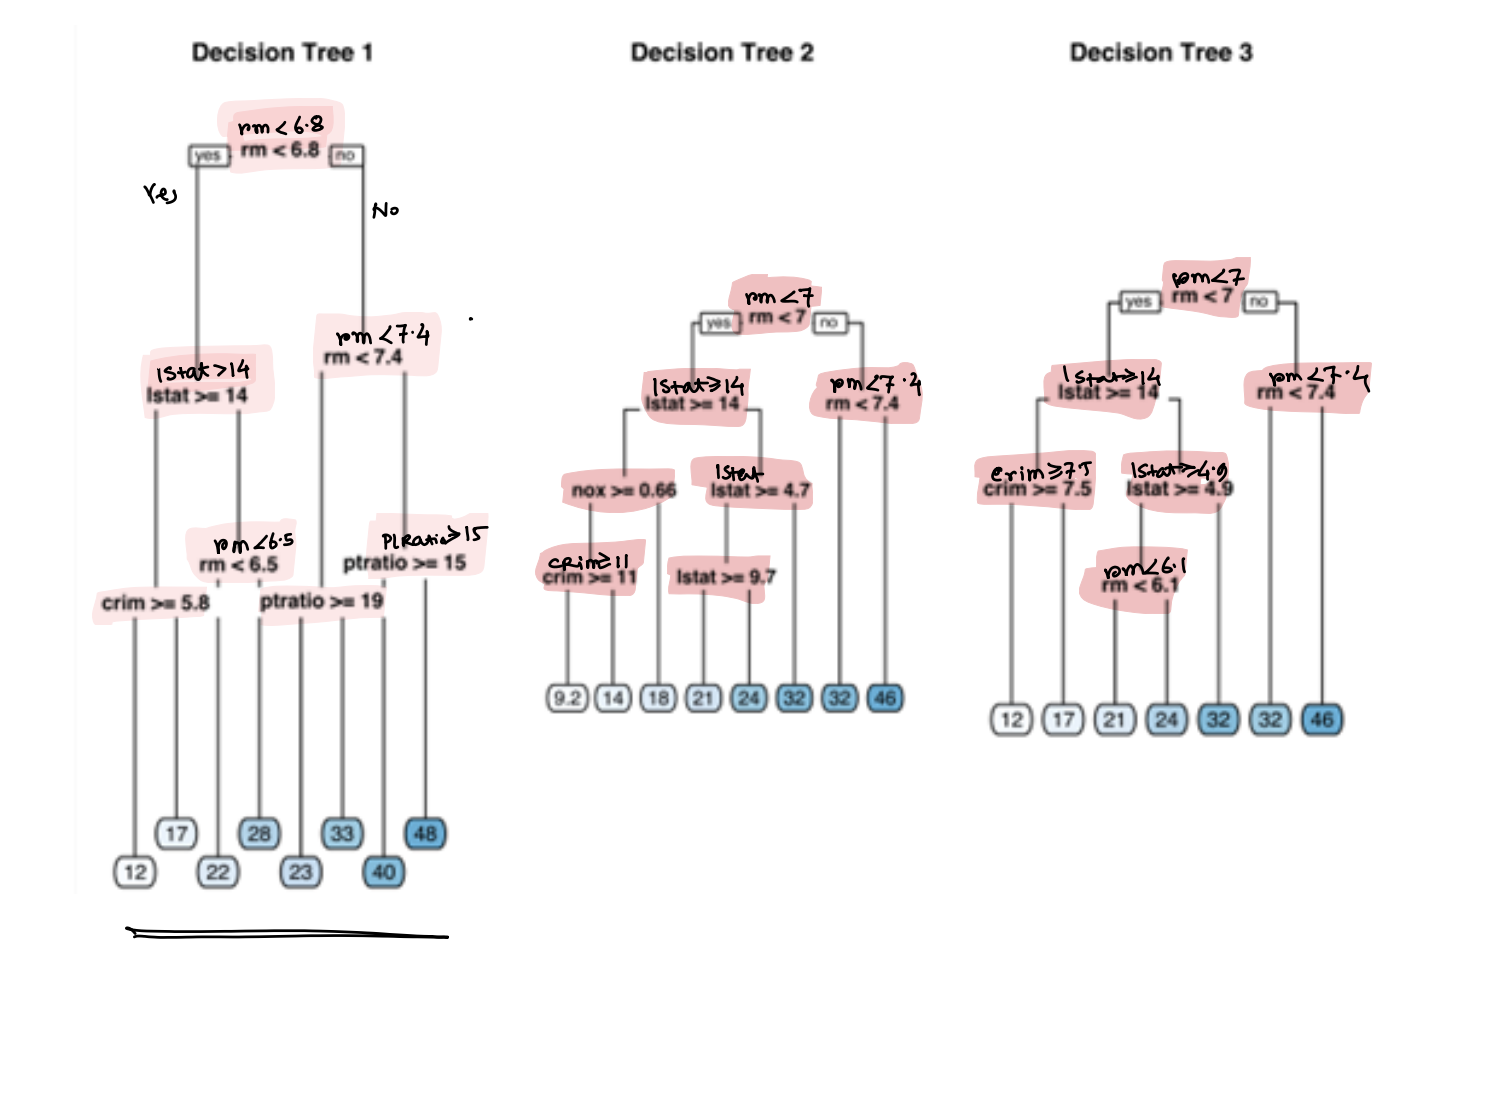
\includegraphics[scale=.22]{fig/Stability_Issues with_Decission_Tree.png}
\end{center}
}\\
\vspace{.1in}
\qBrd[4.5in]{babyblue!50}{
\sqBullet{blue}
Even if a couple of rows of the data are altered/ removed, the algorithm may find significantly different tree as an optimal solution. 
}
\end{frame}



\begin{frame}\frametitle{ Standard Decision Tree may not be robust}
\qBrd[4.5in]{babyblue!50}{
\sqBullet{blue}
The first few partitions may be similar in the top at each trees,  they tend to differ significantly closer to the terminal nodes.  
}\\
\vspace{.1in}
\qBrd[4.5in]{purple!40}{
\sqBullet{blue}
The deeper nodes tend to over-fit the specific attributes of the sample data. Consequently, slight variation in the samples may lead to highly variable mechanism for estimating and  predicting.  
}\\
\vspace{.1in}
\qBrd[4.5in]{applegreen!40}{
\sqBullet{olive}
Bootstrap Aggregating (Bagging) aims to address the instability in estimation and provide more robust solutions. 
}
\end{frame}





{
 \setbeamercolor{background canvas}{bg=}
\includepdf[pages={4}, scale=1]{STAT380-Unit4.pdf}
}


\begin{frame}
\qBrd[4.5in]{babyblueeyes!50}{
\begin{enumerate}
\qBrd[4in]{airforceblue!50}{
\item[\sqBullet{bluebell}]  If $T_1, T_2, \ldots, T_B $ are $ \HLTEQ[orange]{\text{uncorrelated}}$ with $\HLTY{E(T_i)=\mu} $,  and  $\HLTY{\text{Var}(T_i)=\sigma^2} <\infty$, then 
$$   \HLTW{ E(\overline{T})= \mu  },\;\;  \HLTW{\text{var}\left(\overline{T} \right)= \frac{\sigma^2}{B}}$$
where $ \displaystyle \overline{T}= \frac{1}{B} \sum_{i=1}^B T_i $
}\\
\vspace{.1in}
\qBrd[4in]{olive!50}{
\item[\sqBullet{olive}]  The assumption that $Z_i $ are uncorrelated is a crucial assumption $ \HLTEQ[orange]{\text{uncorrelated}}$.
}
\\
\vspace{.1in}
\end{enumerate}
}\\
\vspace{.2in}

\end{frame}


{
 \setbeamercolor{background canvas}{bg=}
\includepdf[pages={5}, scale=1]{STAT380-Unit4.pdf}
}



\begin{frame}\frametitle{Bootstrap: An Example}
\qBrd[4.5in]{babyblue!50}{
\begin{center}
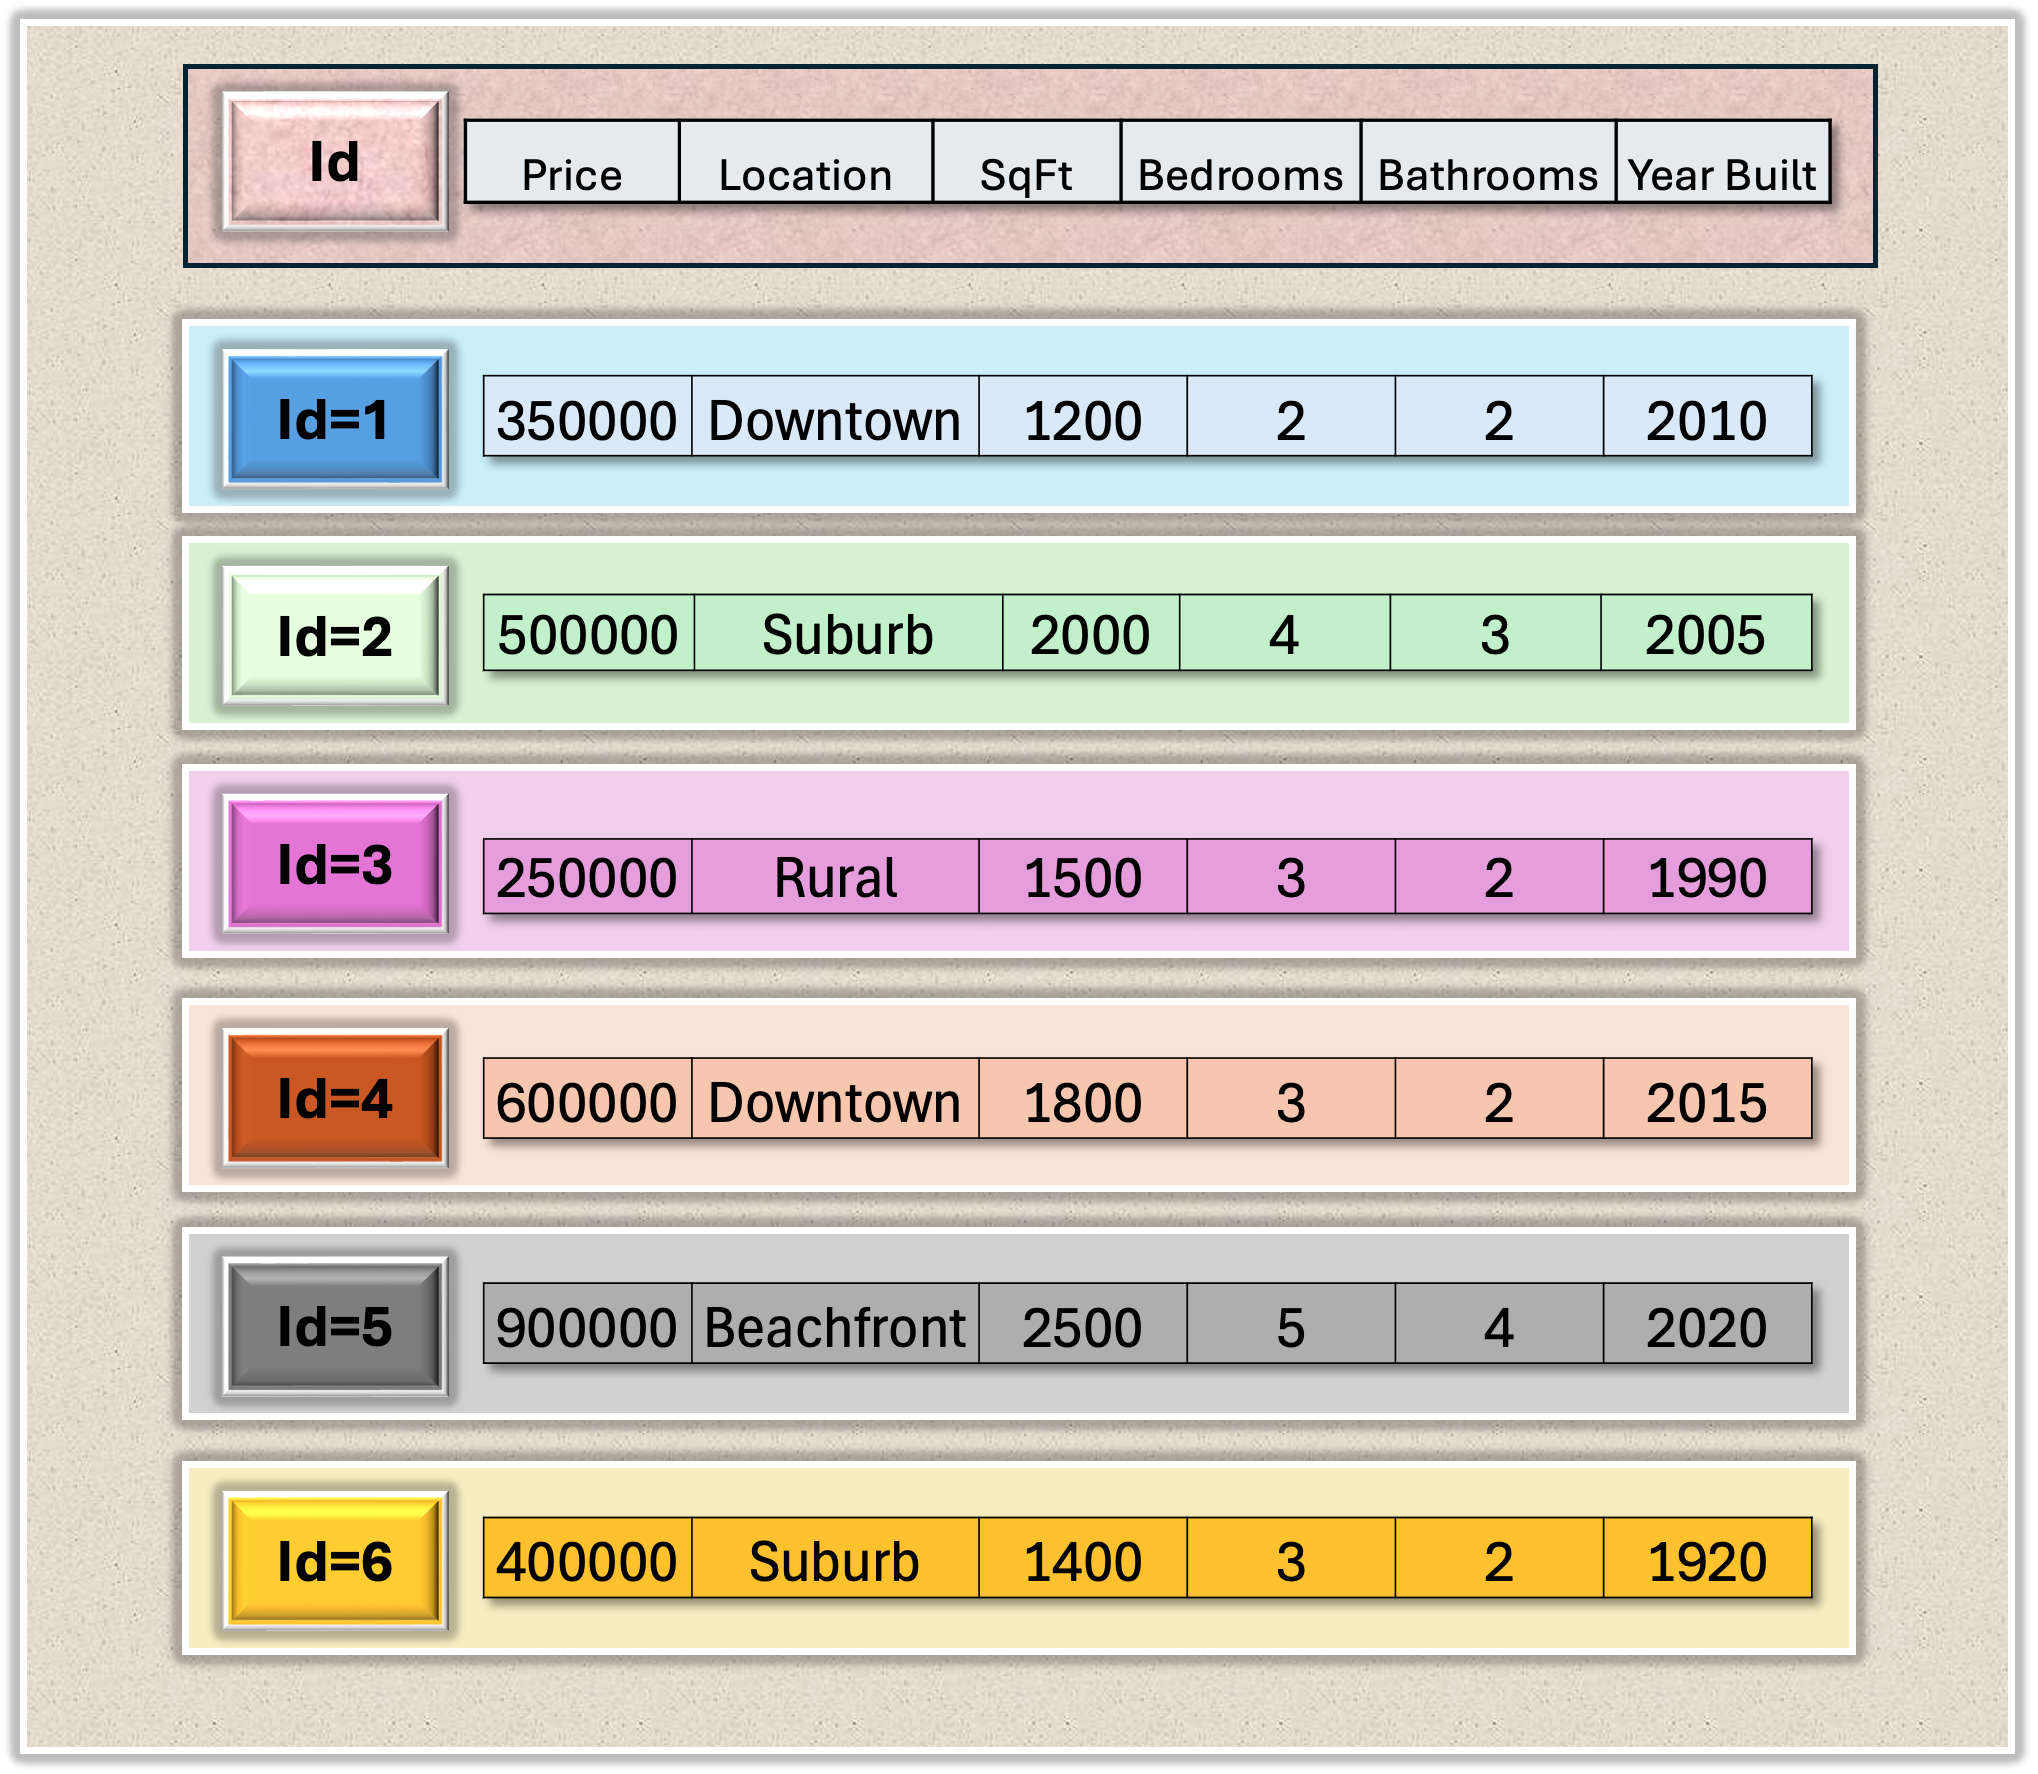
\includegraphics[scale=.22]{fig/Sim_data_Bootstrap.png}
\end{center}
}\\
\vspace{1in}
\end{frame}


\begin{frame}\frametitle{Bootstrap: An Example}
\qBrd[4.5in]{slateblue!50}{
\begin{center}
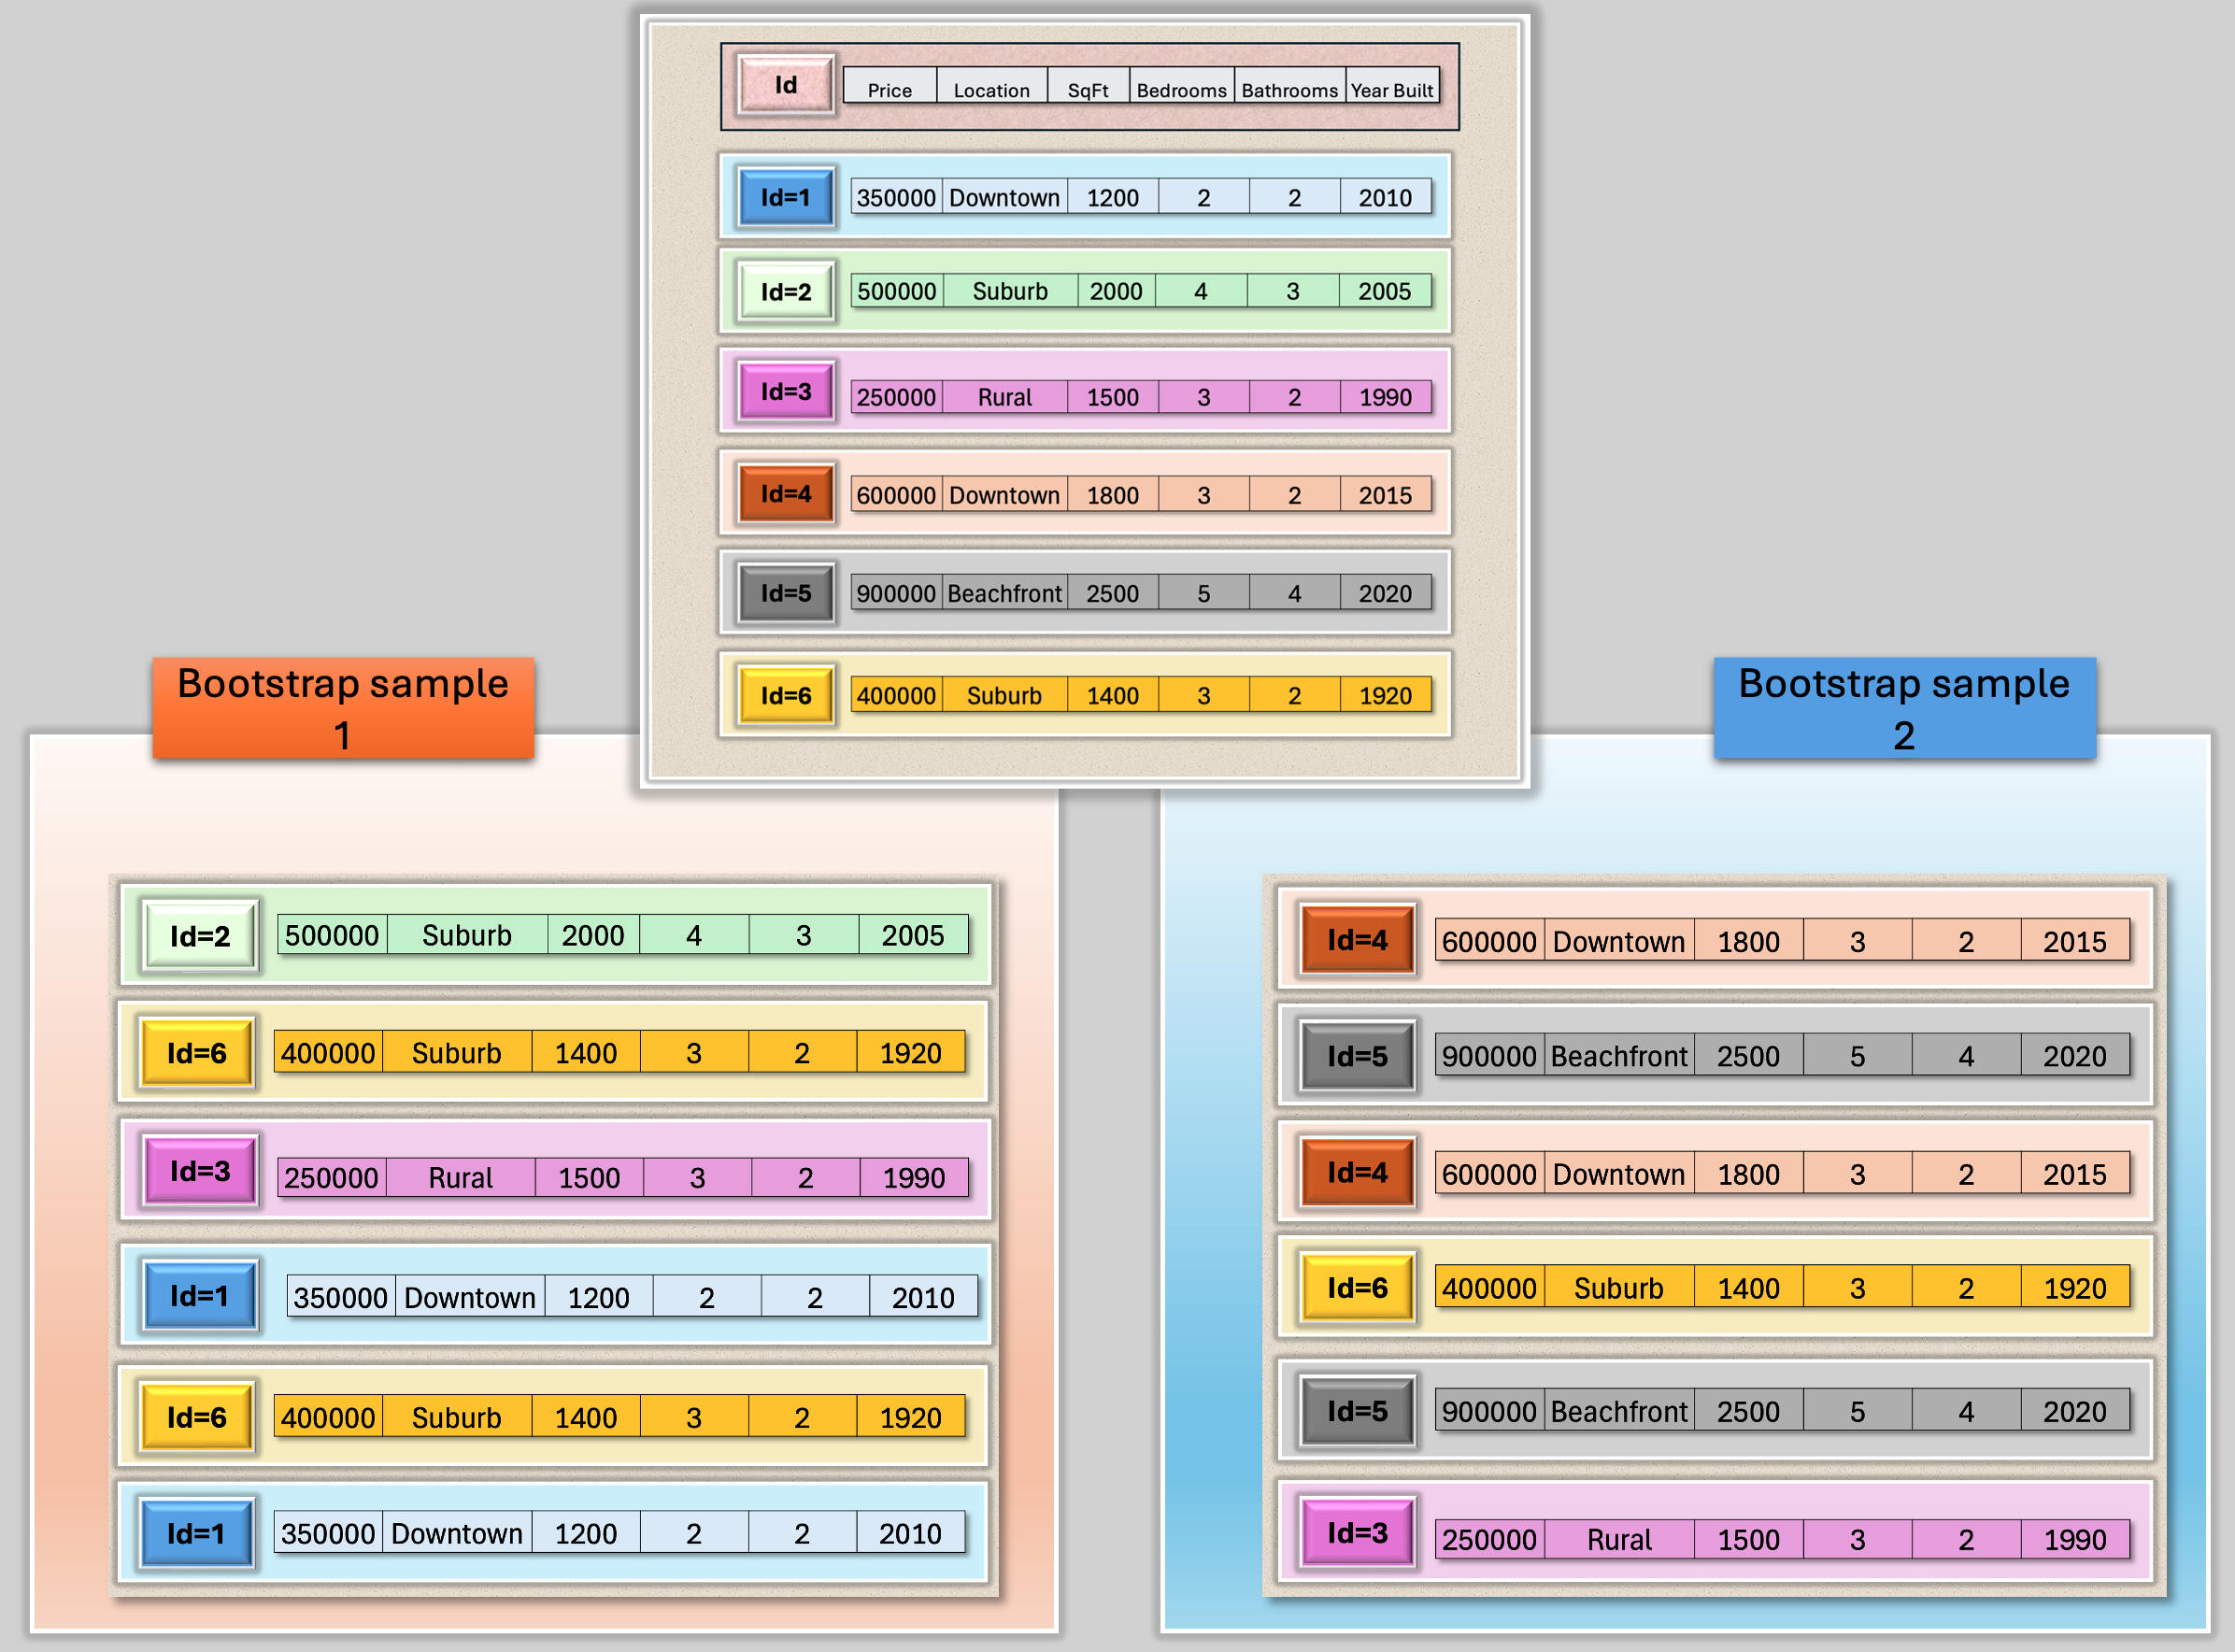
\includegraphics[scale=.24]{fig/Sim_BootstrapSample.png}
\end{center}
}\\
\vspace{1in}
\end{frame}



\begin{frame}\frametitle{Bootstrap Samples: An Example}
\vspace{.4in}
\qBrd[4.5in]{slateblue!50}{
\begin{center}
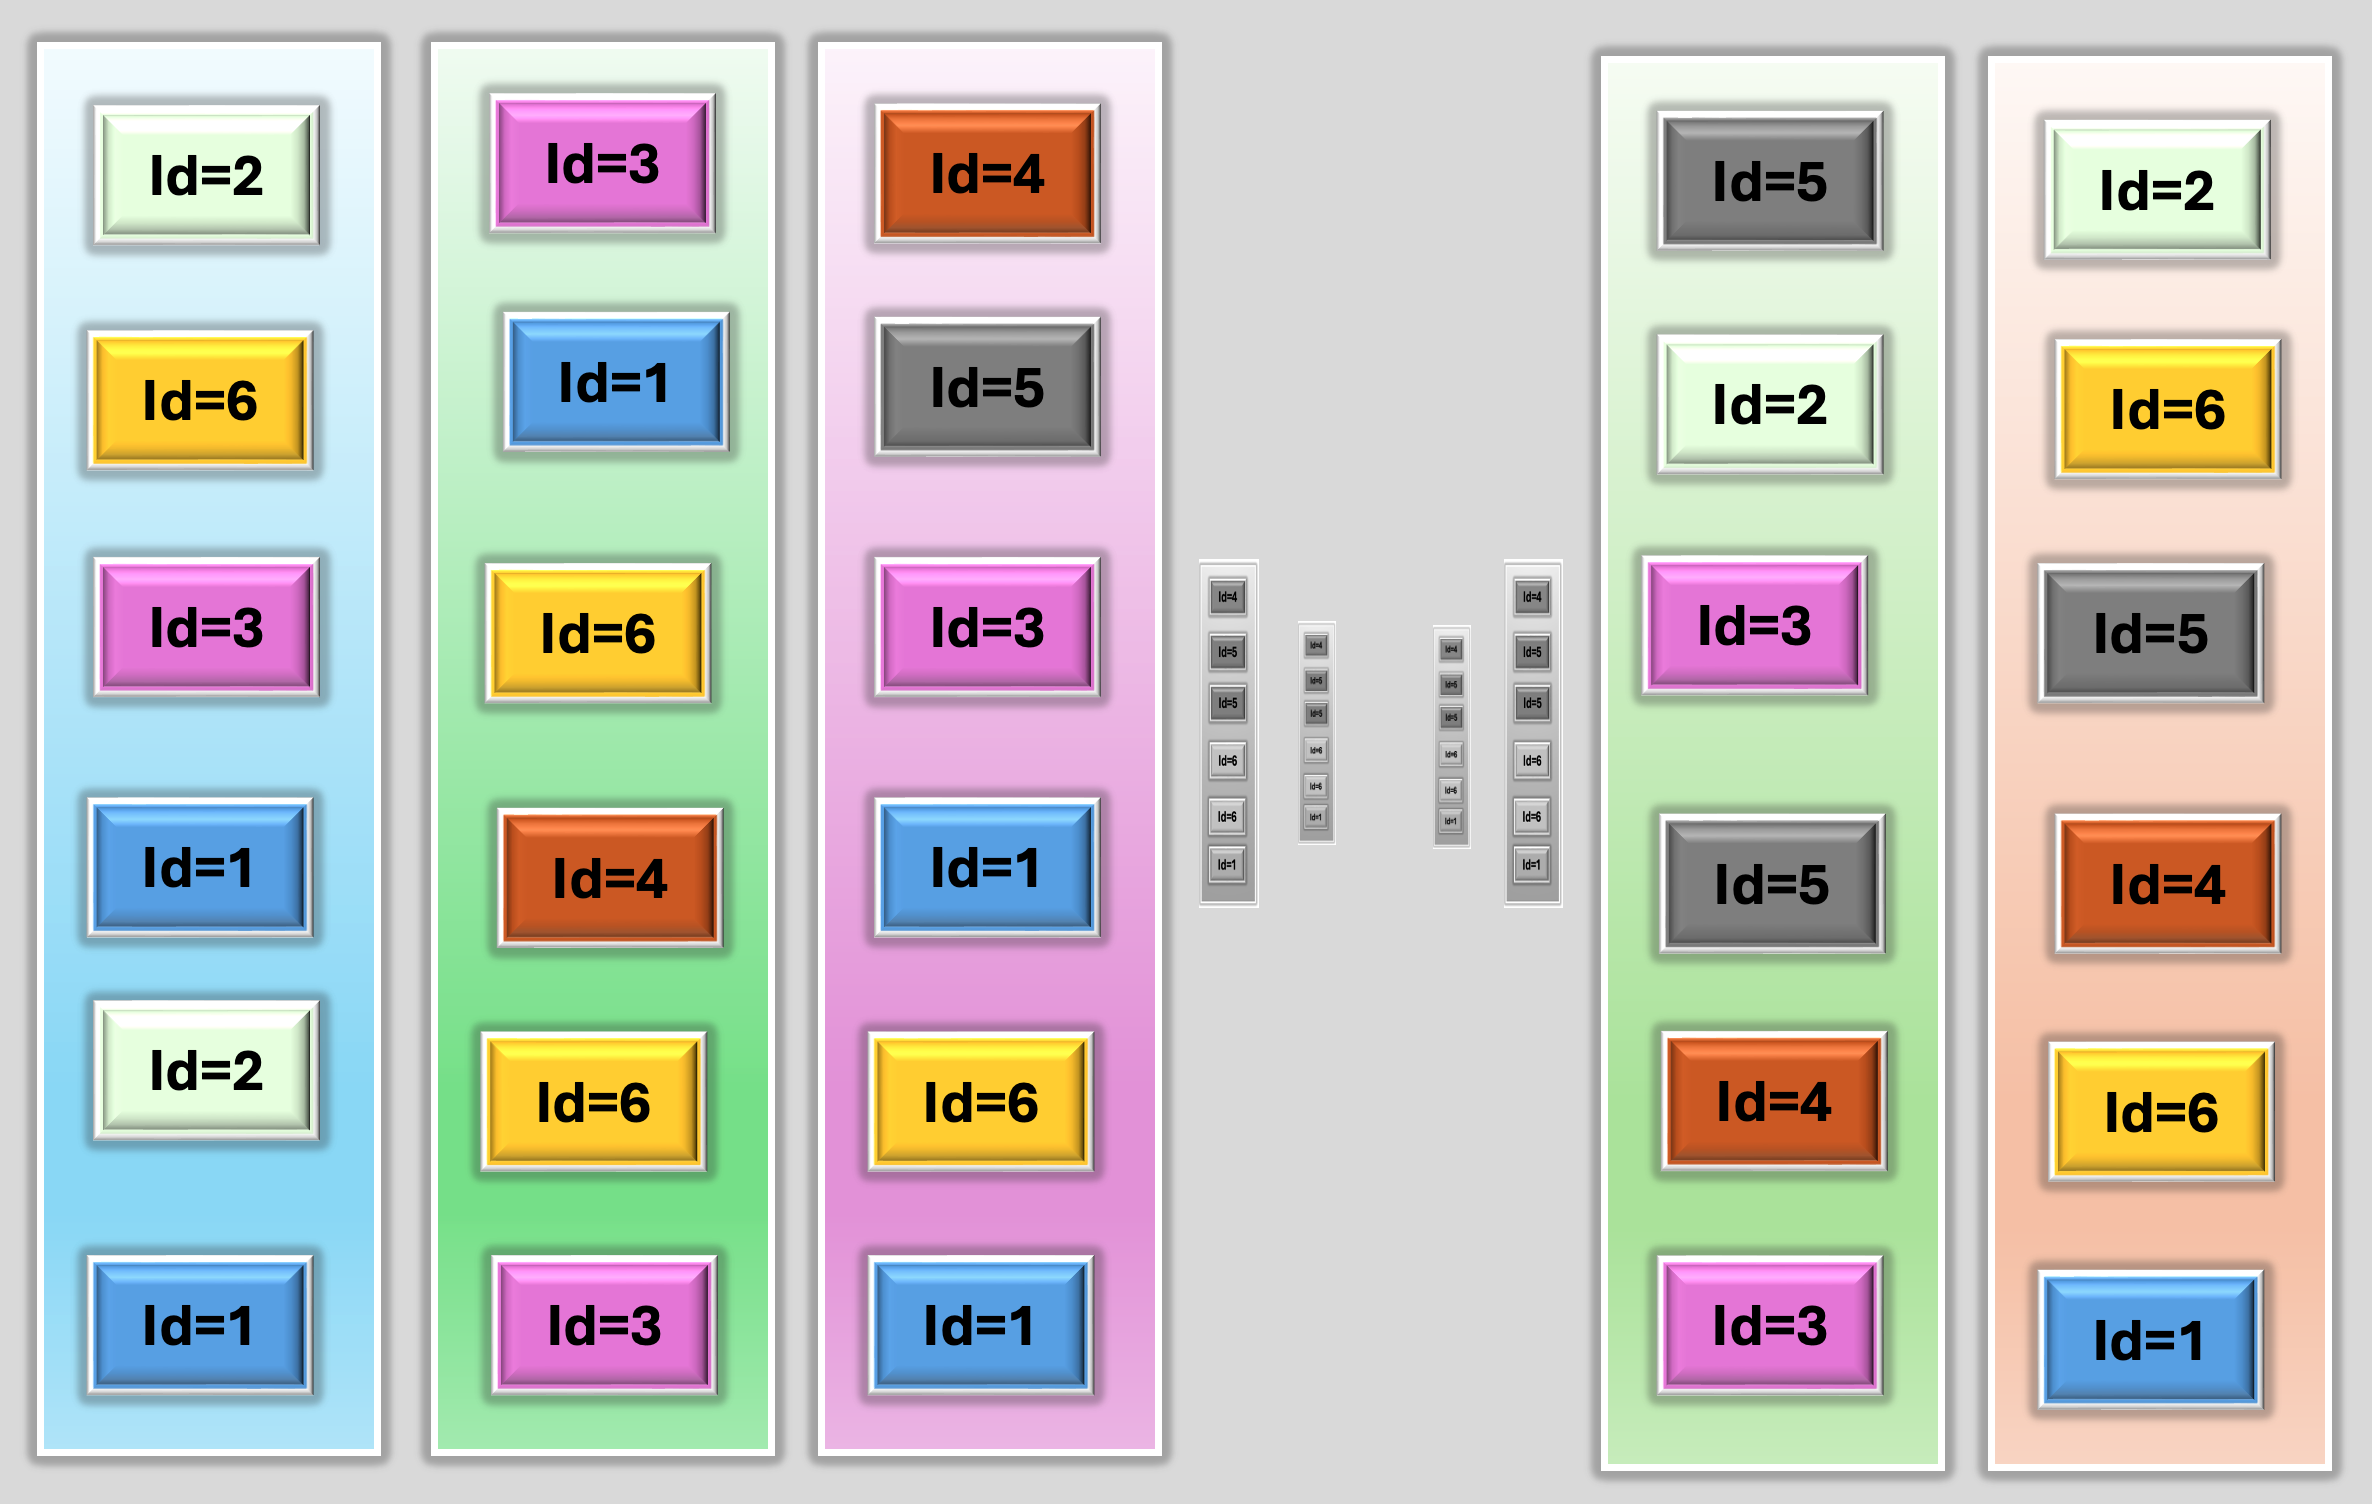
\includegraphics[scale=.24]{fig/Bootstrap Samples_id.png}
\end{center}
}\\
\end{frame}

{
 \setbeamercolor{background canvas}{bg=}
\includepdf[pages={7-8}, scale=1]{STAT380-Unit4.pdf}
}



\begin{frame}\frametitle{Bagging: Bootstrap Aggregation}
\qBrd[4.5in]{slateblue!50}{
\begin{center}
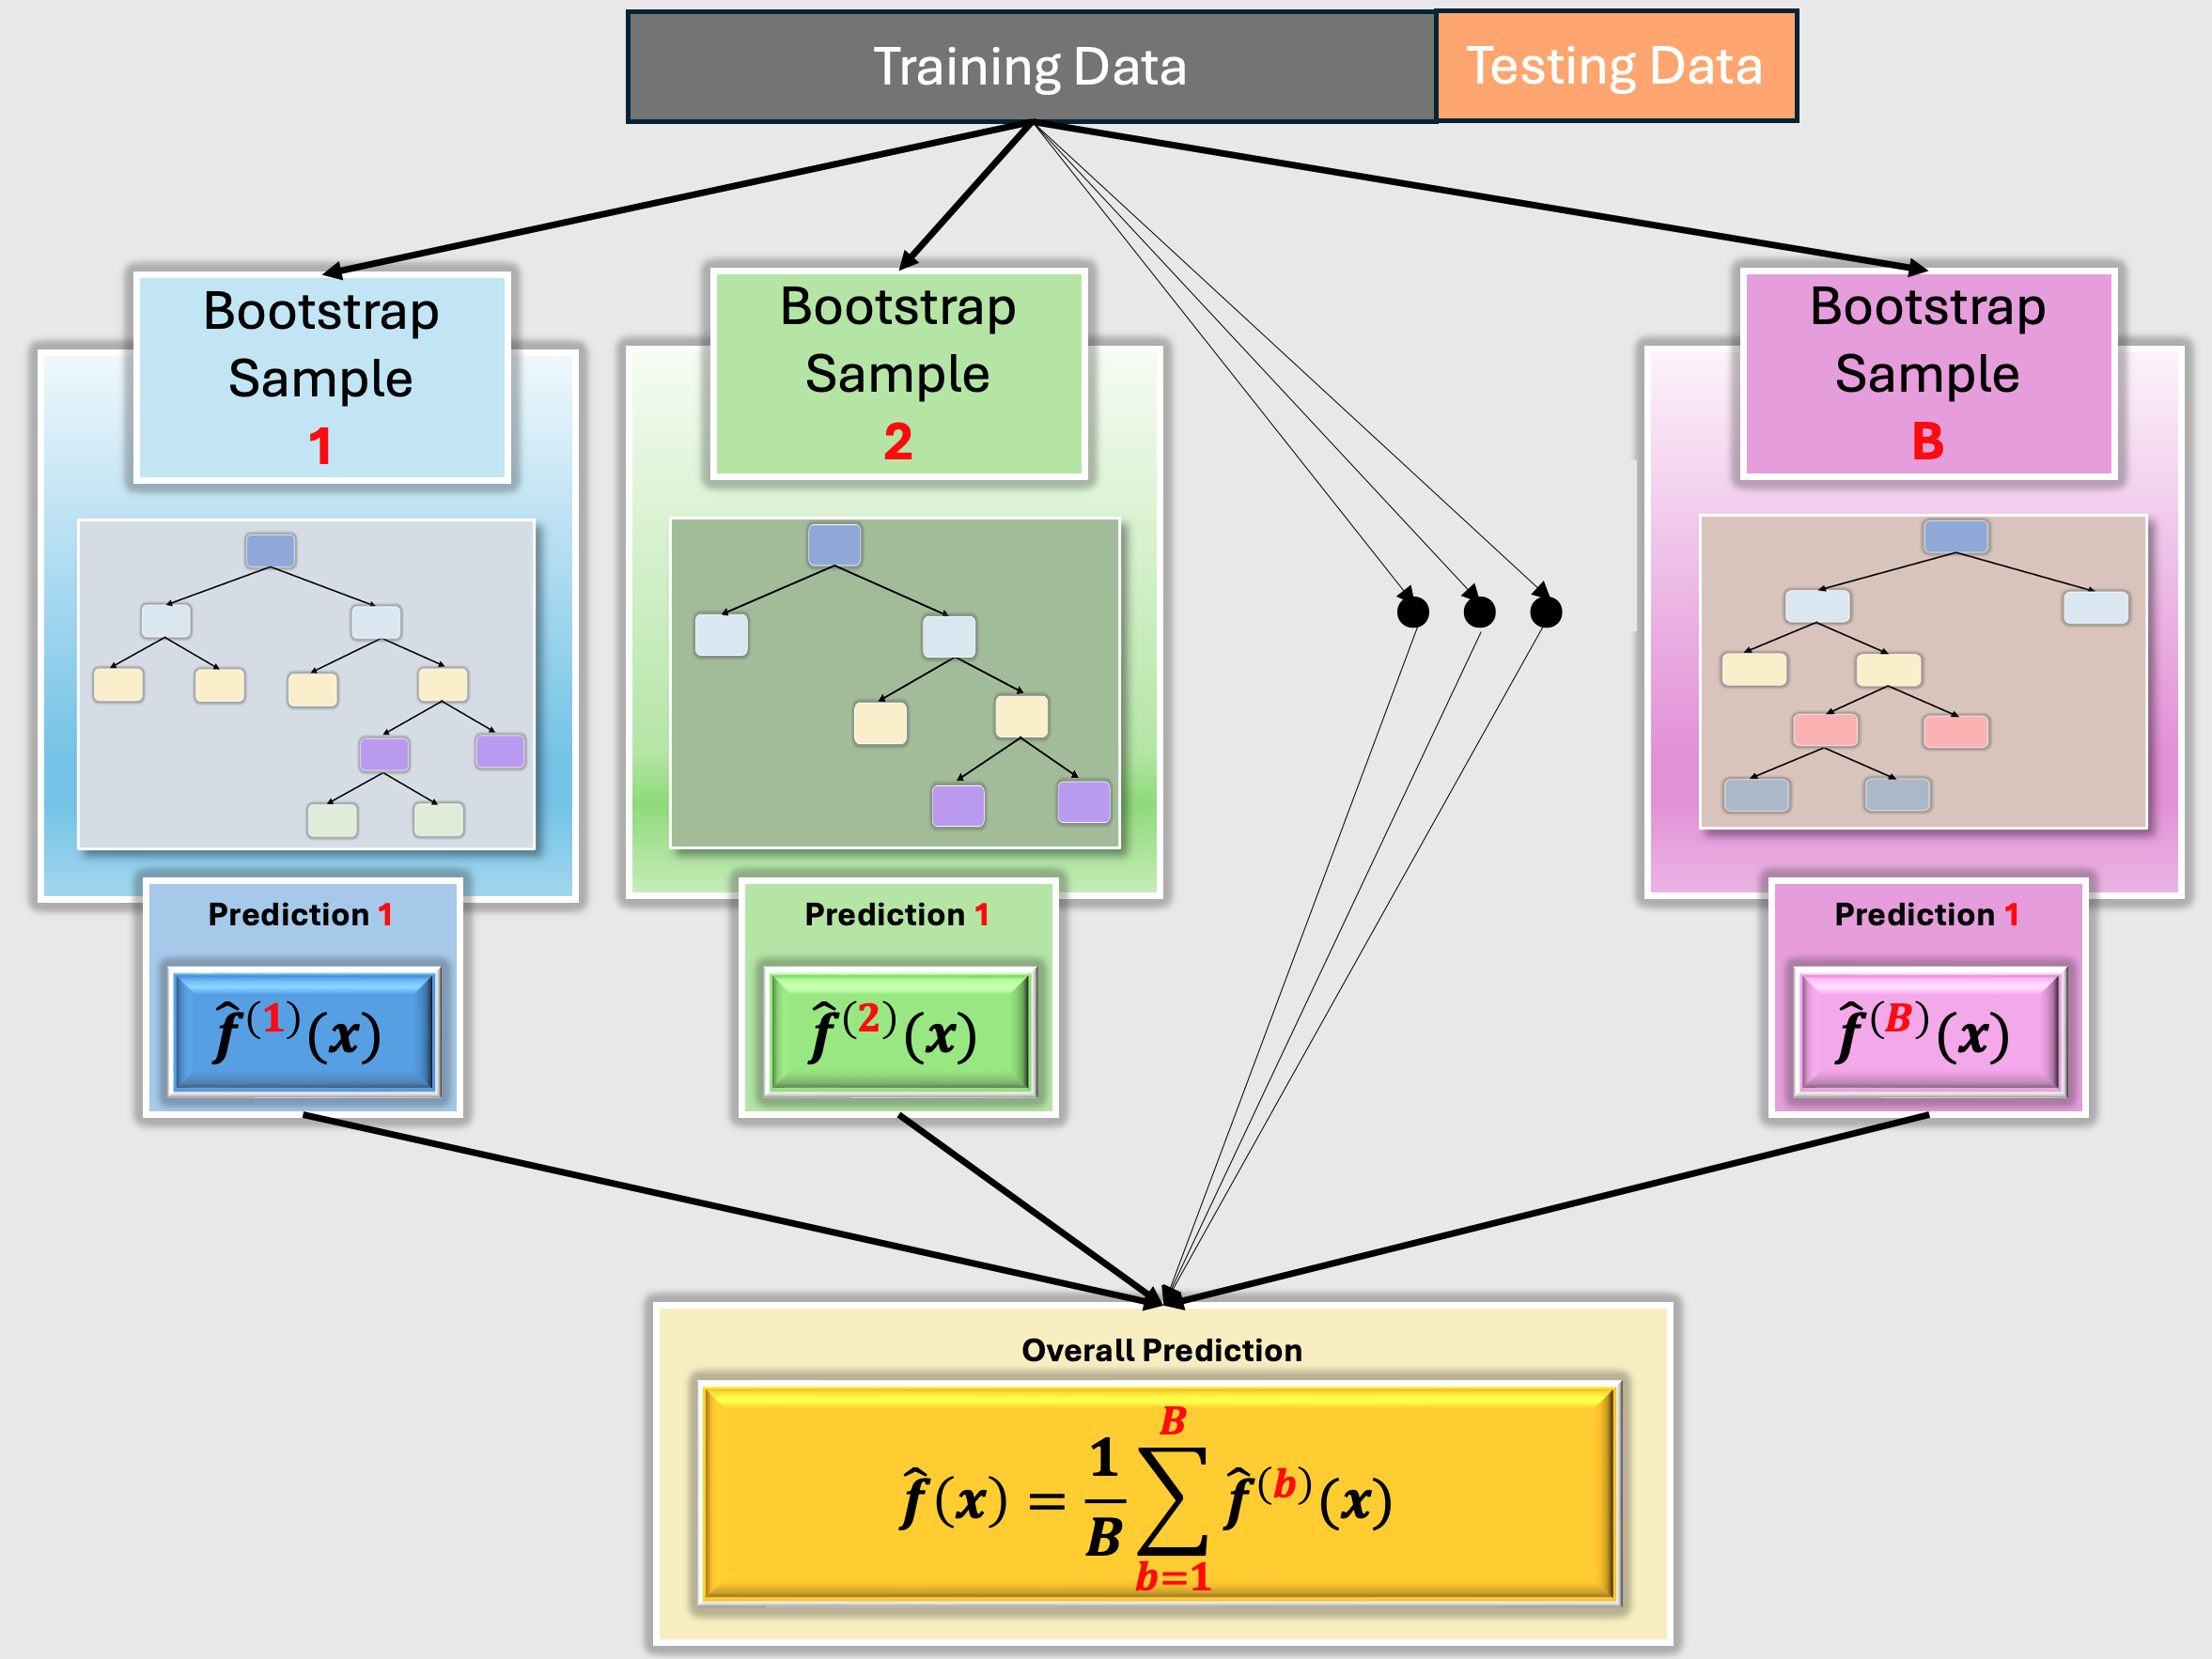
\includegraphics[scale=.24]{fig/Bagging_Estimator.png}
\end{center}
}\\
\end{frame}




{
 \setbeamercolor{background canvas}{bg=}
\includepdf[pages={9}, scale=1]{STAT380-Unit4.pdf}
}


\begin{frame}\frametitle{ Importance Measure of a Variable}
\qBrd[4.5in]{babyblue!50}{
\sqBullet{blue}
For a single tree, we can add up  the decrements  in Sum of Squared Errors associated with all the splits of a particular variable. 
}\\
\vspace{.1in}
\qBrd[4.5in]{purple!40}{
\sqBullet{blue}
For a Random Forest or Bagged trees we aggregate the sum of squared errors for all the trees in a Random Forest or Bagged Trees. 
}\\
\vspace{.1in}
\qBrd[4.5in]{applegreen!40}{
\sqBullet{olive}
There are R functions,  ``importance($\cdot$)'', and ``varImpPlot($\cdot$)'' in the ``randomForest''  R-package. 
}
\end{frame}





\begin{frame}\frametitle{ Relation Between a Variable and the Response}
\qBrd[4.5in]{babyblue!50}{
\sqBullet{blue}
A standard practice is to compute the average value of a prediction function for a fixed value of the target variable, while averaged over all the other variables. 
}\\
\vspace{.1in}
\qBrd[4.5in]{purple!40}{
\sqBullet{blue}
The above procedure is repeated over a range of values of the target variable, and is plotted to visualize the relation between a covariate and the response variable. 
}\\
\end{frame}

{
 \setbeamercolor{background canvas}{bg=}
\includepdf[pages={10-12}, scale=1]{STAT380-Unit4.pdf}
}


\section{Random Forest}
\TransitionFrame[airforceblue]{\Large Random Forest }

%{
% \setbeamercolor{background canvas}{bg=}
%\includepdf[pages={13}, scale=1]{STAT380-Unit4.pdf}
%}



\begin{frame}\frametitle{Correlated or Not?}
\qBrd[4.7in]{slateblue!50}{
\begin{center}
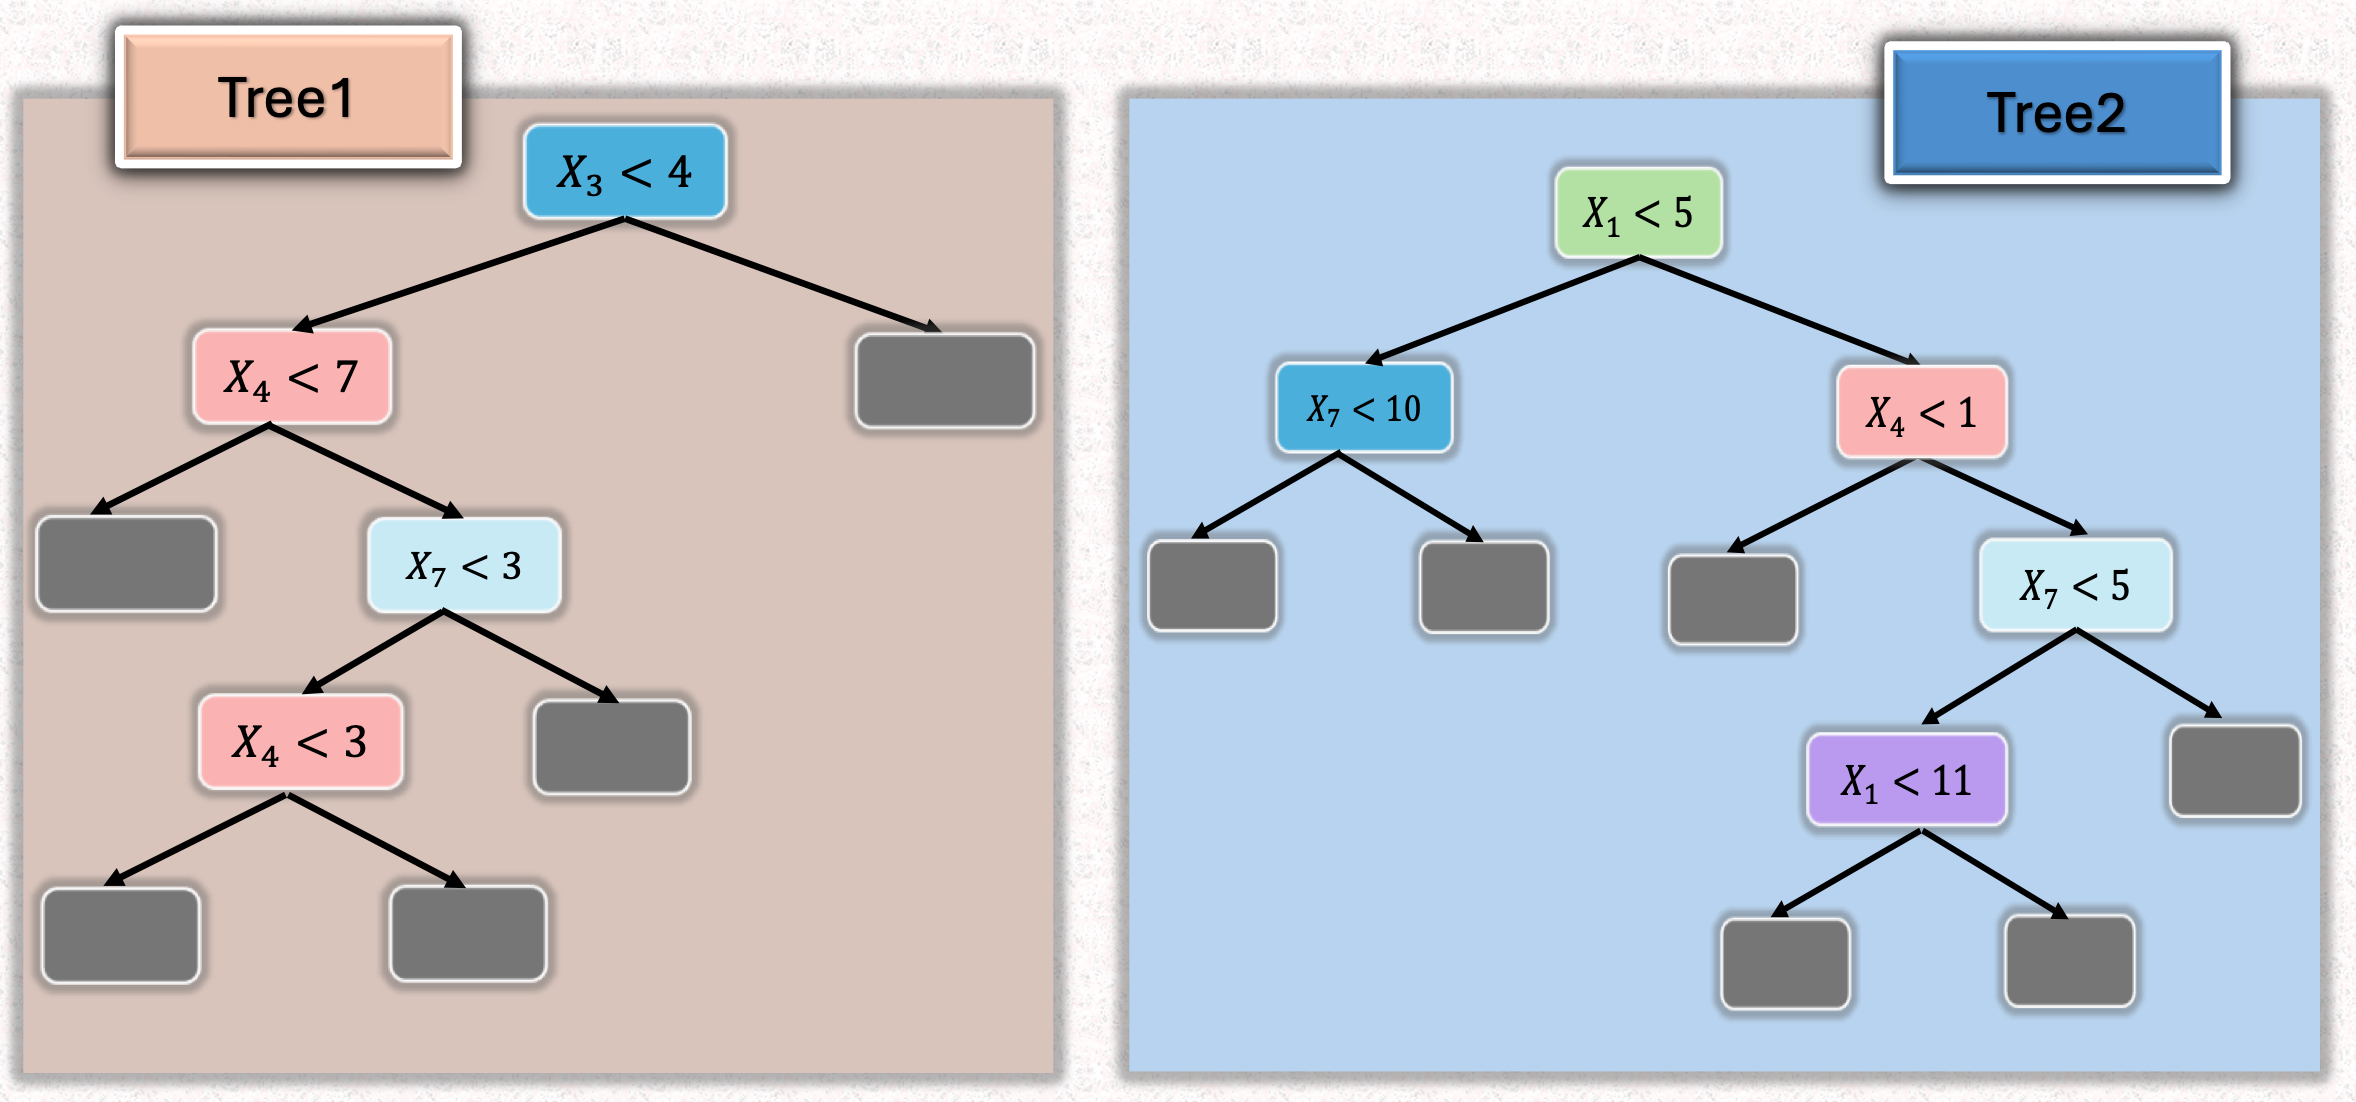
\includegraphics[scale=.28]{fig/Indep Tree.png}
\end{center}
}\\
\vspace{1in}
\end{frame}



\begin{frame}\frametitle{Correlated or Not?}
\qBrd[4.5in]{slateblue!50}{
\begin{center}
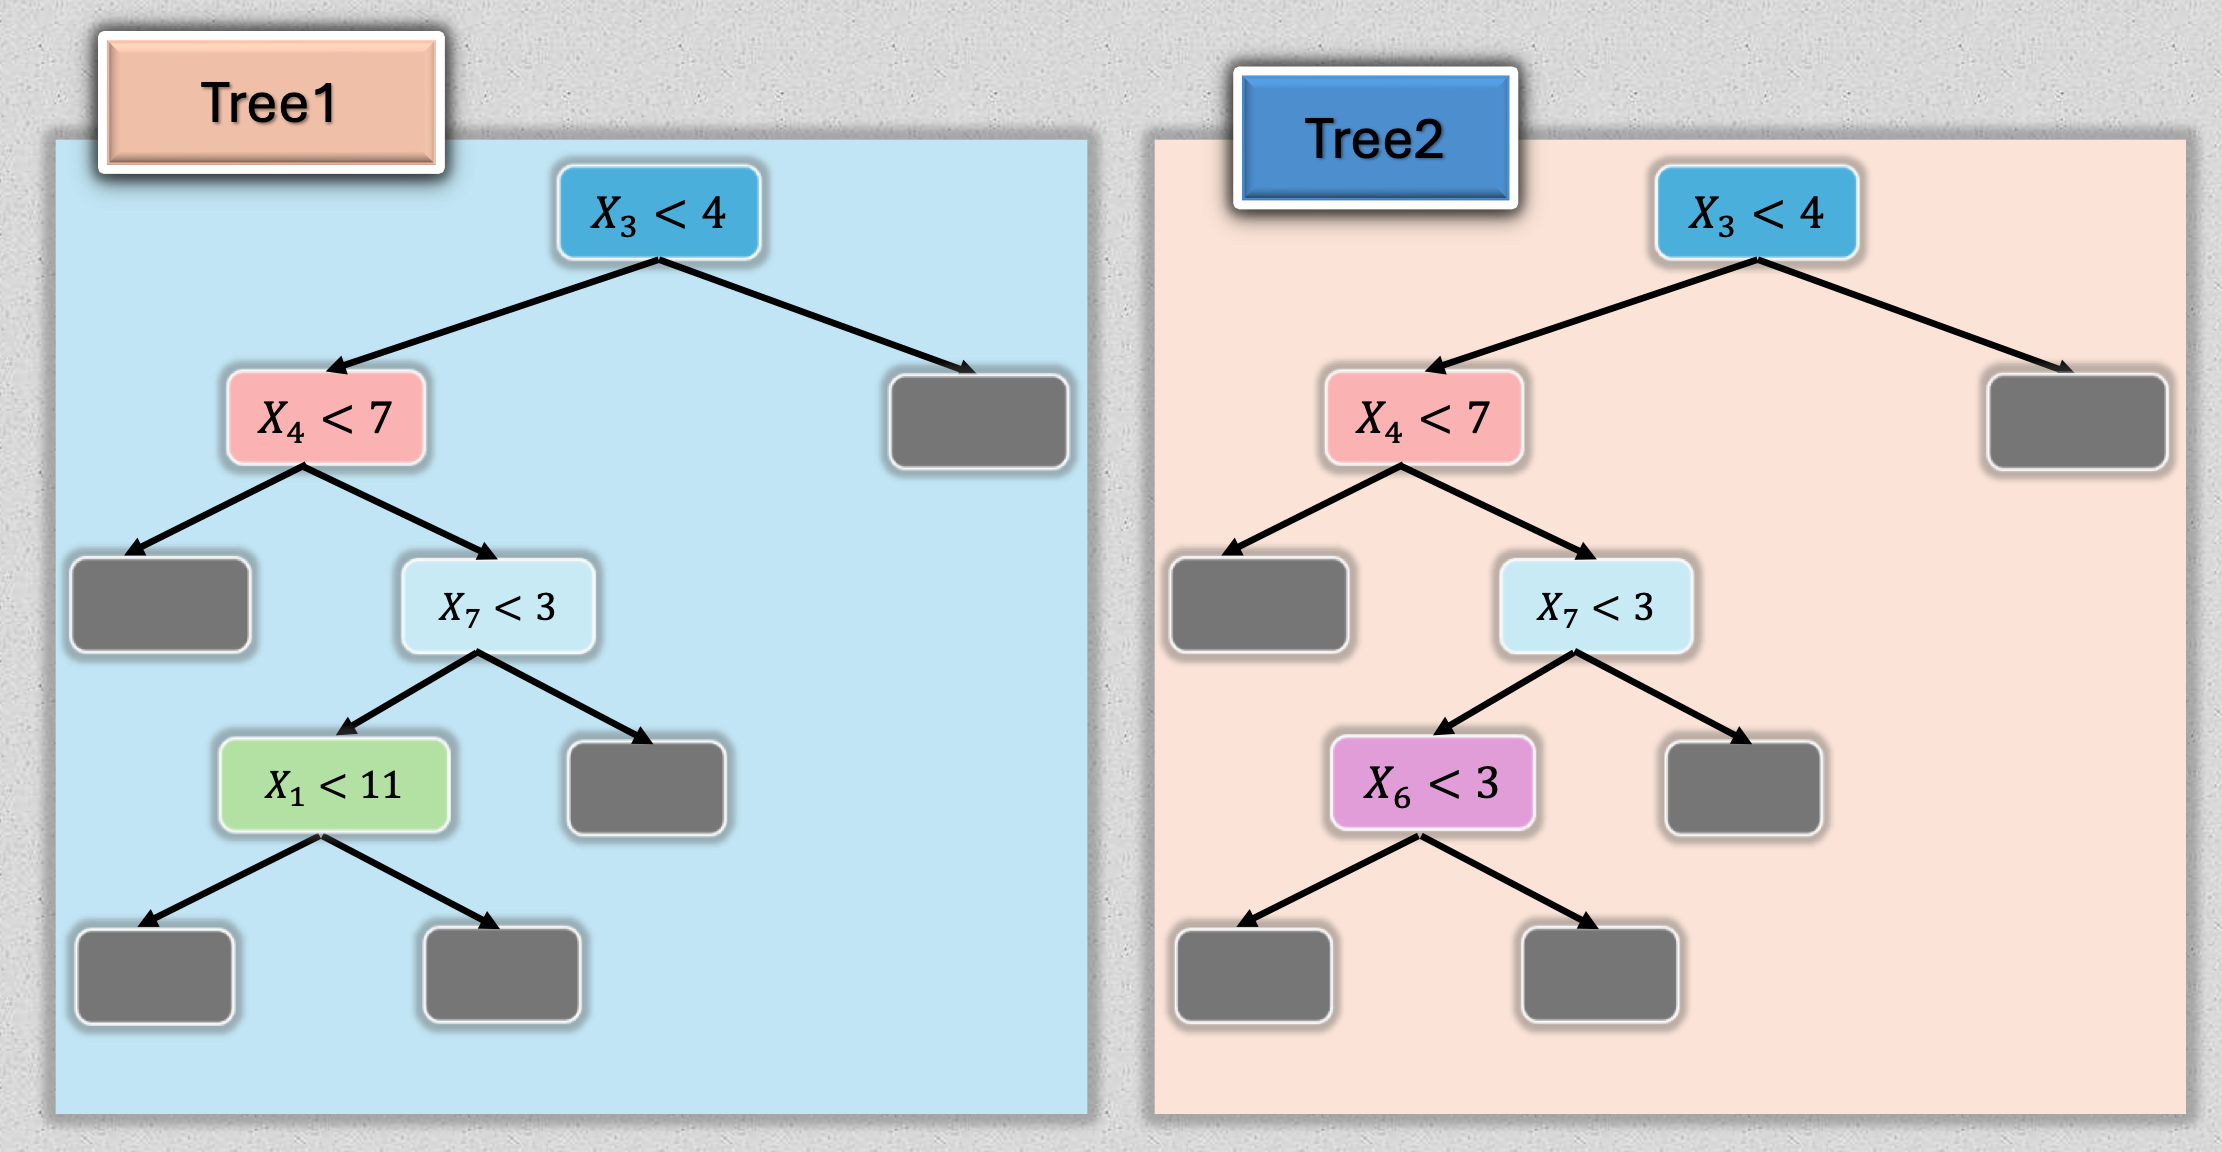
\includegraphics[scale=.28]{fig/Dependent Tree.png}
\end{center}
}\\
\vspace{1in}
\end{frame}





\begin{frame}
\qBrd[4.5in]{babyblueeyes!50}{
\begin{enumerate}
\qBrd[4in]{airforceblue!50}{
\item[\sqBullet{bluebell}]  If $T_1, T_2, \ldots, T_B $ are $ \HLTEQ[orange]{\text{uncorrelated}}$ with $\HLTY{E(T_i)=\mu} $,  and  $\HLTY{\text{Var}(T_i)=\sigma^2} <\infty$, then 
$$   \HLTW{ E(\overline{T})= \mu  },\;\;  \HLTW{\text{var}\left(\overline{T} \right)= \frac{\sigma^2}{B}}$$
where $ \displaystyle \overline{T}= \frac{1}{B} \sum_{i=1}^B T_i $
}\\
\vspace{.1in}
\qBrd[4in]{olive!50}{
\item[\sqBullet{olive}]  The assumption that $T_i $ are uncorrelated is a crucial assumption $ \HLTEQ[orange]{\text{uncorrelated}}$.
}
\\
\vspace{.1in}
\end{enumerate}
}\\
\vspace{.2in}

\end{frame}




\begin{frame}\frametitle{How Correlation Affect the Variance of Sample Mean? A Special Case}
\qBrd[4.5in]{babyblueeyes!50}{
\begin{enumerate}
\qBrd[4in]{airforceblue!50}{
\item[\sqBullet{bluebell}]  If $T_1, T_2, \ldots, T_B $ are $ \HLTEQ[red!50]{\text{correlated}}$ with $\HLTY{E(T_i)=\mu} $,  and  $\HLTY{\text{Var}(T_i)=\sigma^2} <\infty$, $\HLTW{\text{cor}(T_i, T_j)=\HLTEQ[byzantine!40]{\rho>0}}$, then 
$$   \HLTW{ E(\overline{T})= \mu  },\;\;  \HLTW{\text{var}\left(\overline{T} \right)= \left( \frac{1-\HLTEQ[byzantine!40]{\rho}}{B}+ \HLTEQ[byzantine!40]{\rho}\right)\sigma^2  }$$
where $ \displaystyle \HLTW{ \overline{T}= \frac{1}{B}\sum_{i=1}^{B}T_i  }$
}\\
\vspace{.1in}
\qBrd[4in]{olive!50}{
\item[\sqBullet{olive}]   If $\rho\approx 1, \rho<1$, then  $ \displaystyle \HLTW{\text{var} \left(\overline{T} \right)\approx \sigma^2}$\\
$ \HLTEQ[red!40]{\text{Average has almost same variability of a single TREE}}$.   The Average does not lead to any significant improvement, and the predicted values are not very stable.  
}
\\
\vspace{.1in}
\end{enumerate}
}\\
\vspace{.2in}

\end{frame}


{
 \setbeamercolor{background canvas}{bg=}
\includepdf[pages={14}, scale=1]{STAT380-Unit4.pdf}
}

\begin{frame}\frametitle{Random Forest}
\qBrd[4.5in]{slateblue!50}{
\begin{center}
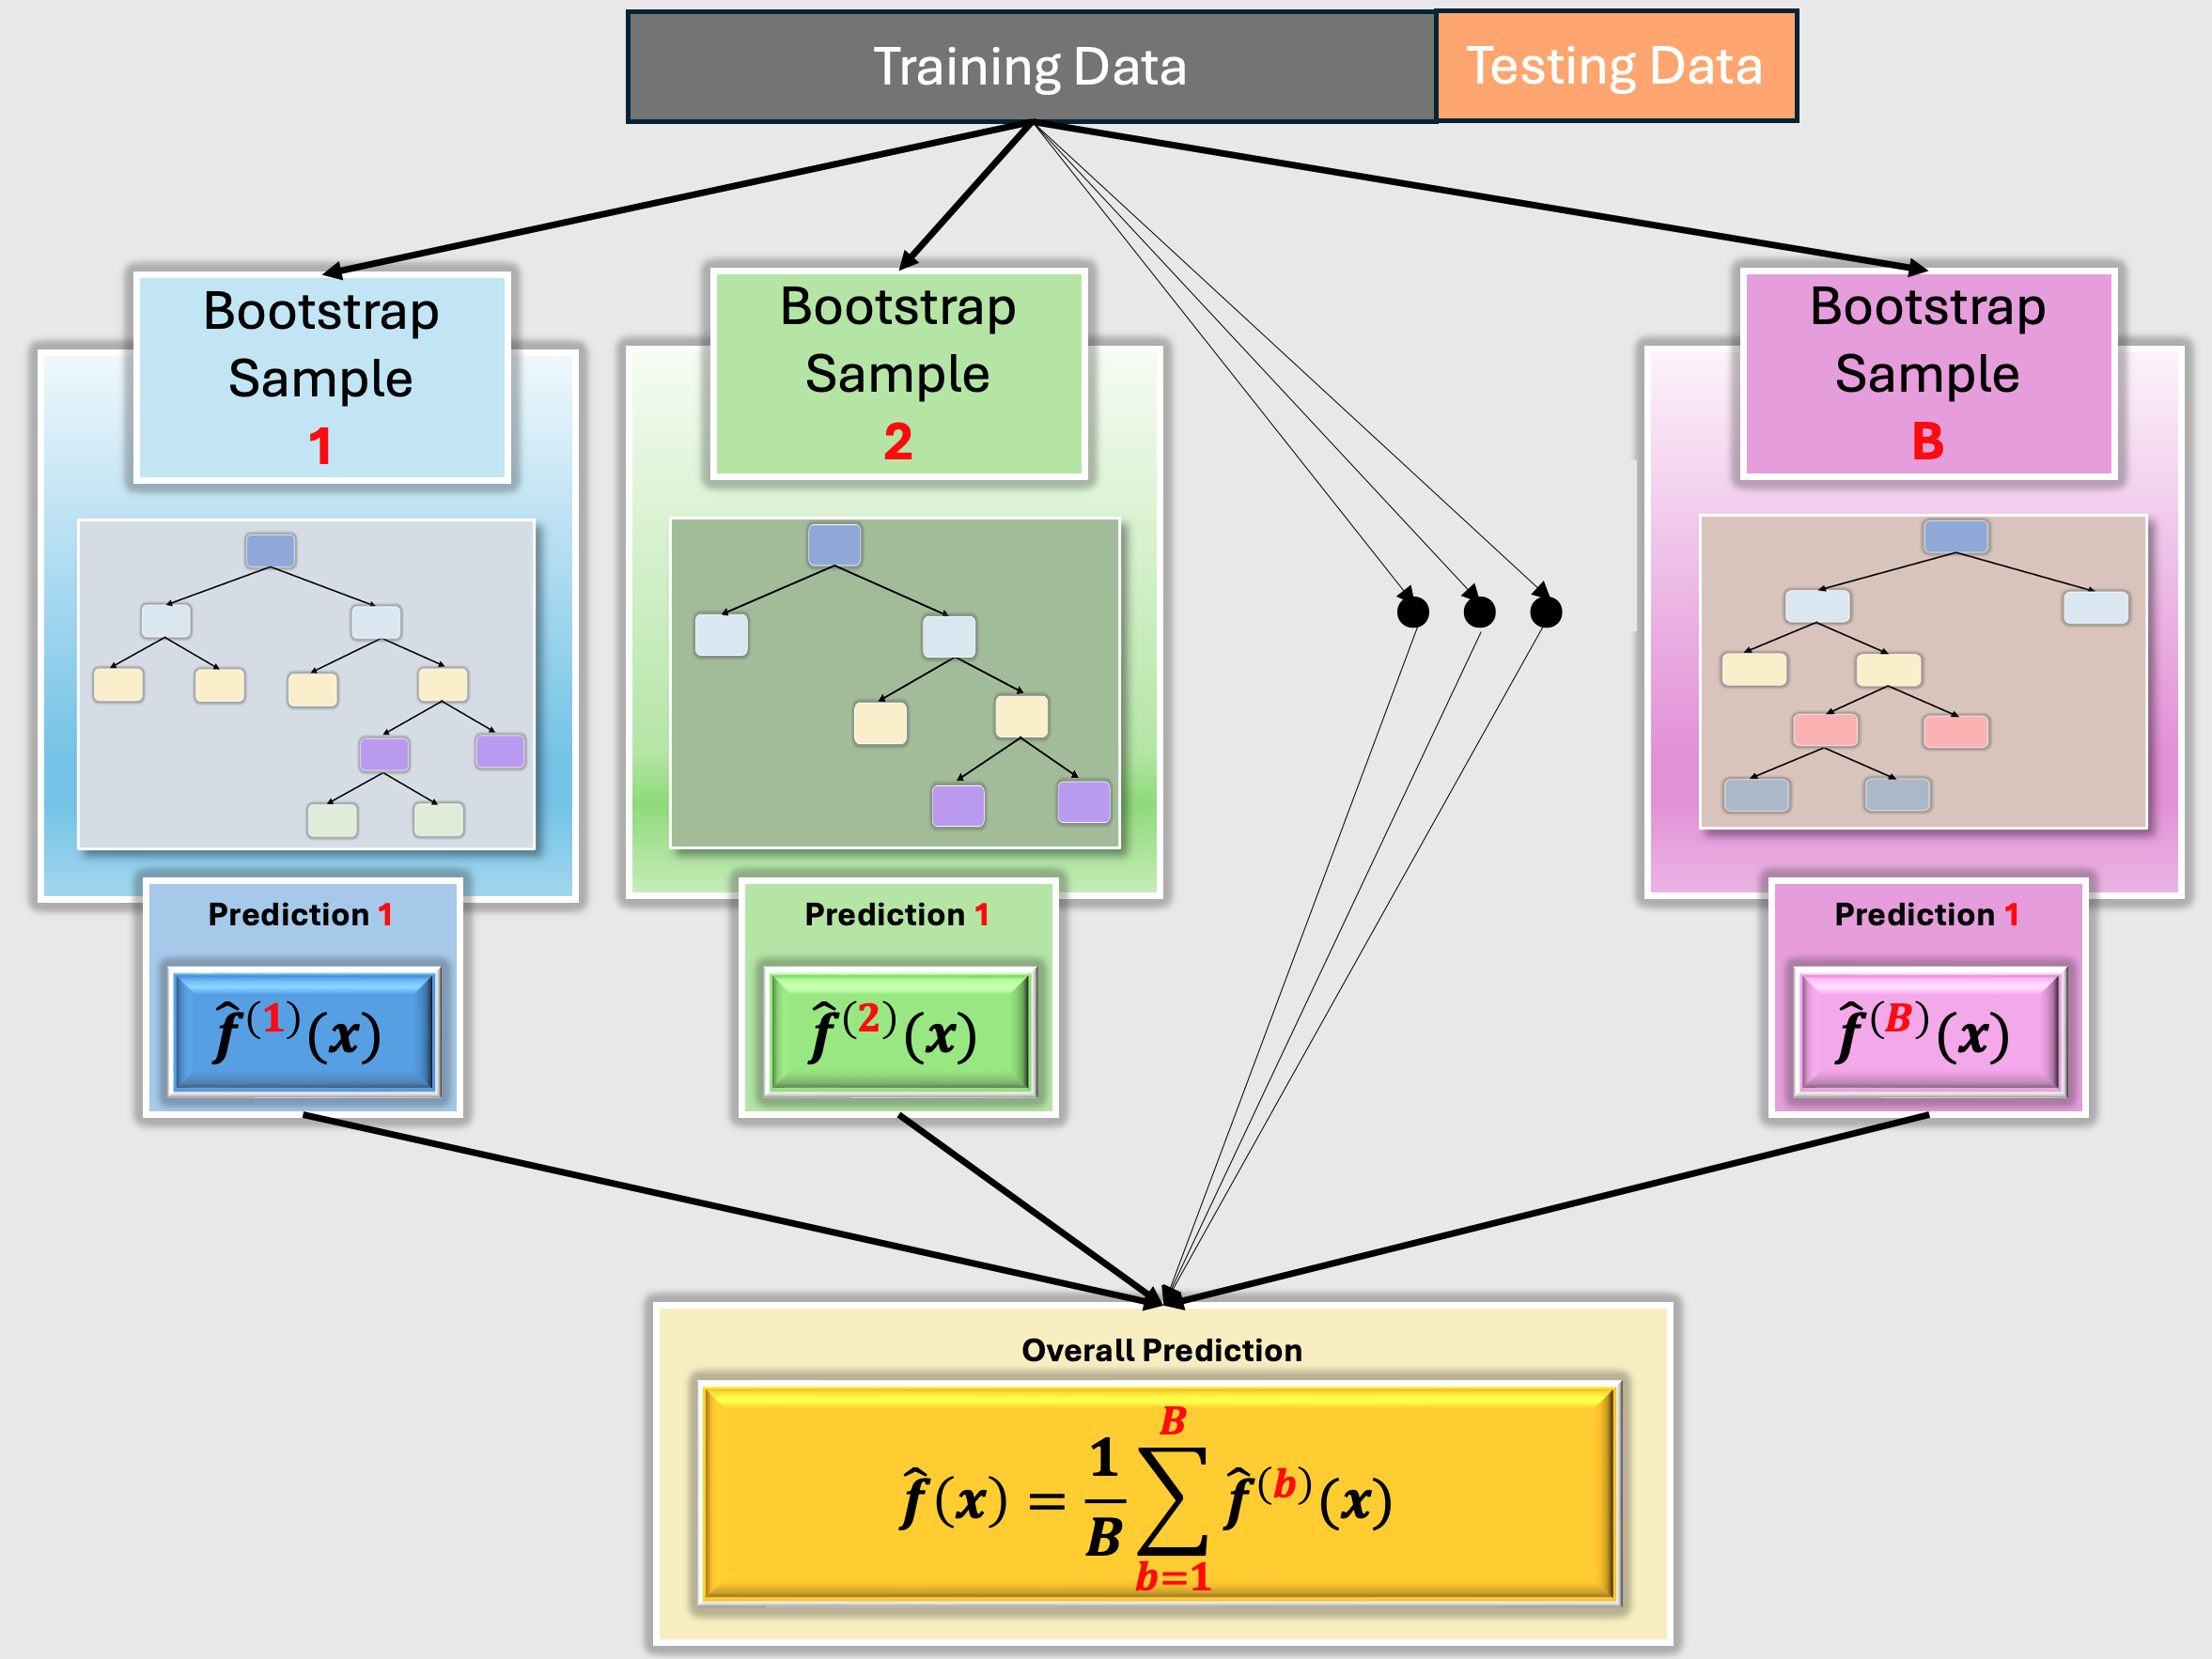
\includegraphics[scale=.24]{fig/Bagging_Estimator.png}
\end{center}
}\\
\end{frame}


\begin{frame}\frametitle{Random Forest}
\qBrd[4.5in]{slateblue!50}{
\begin{center}
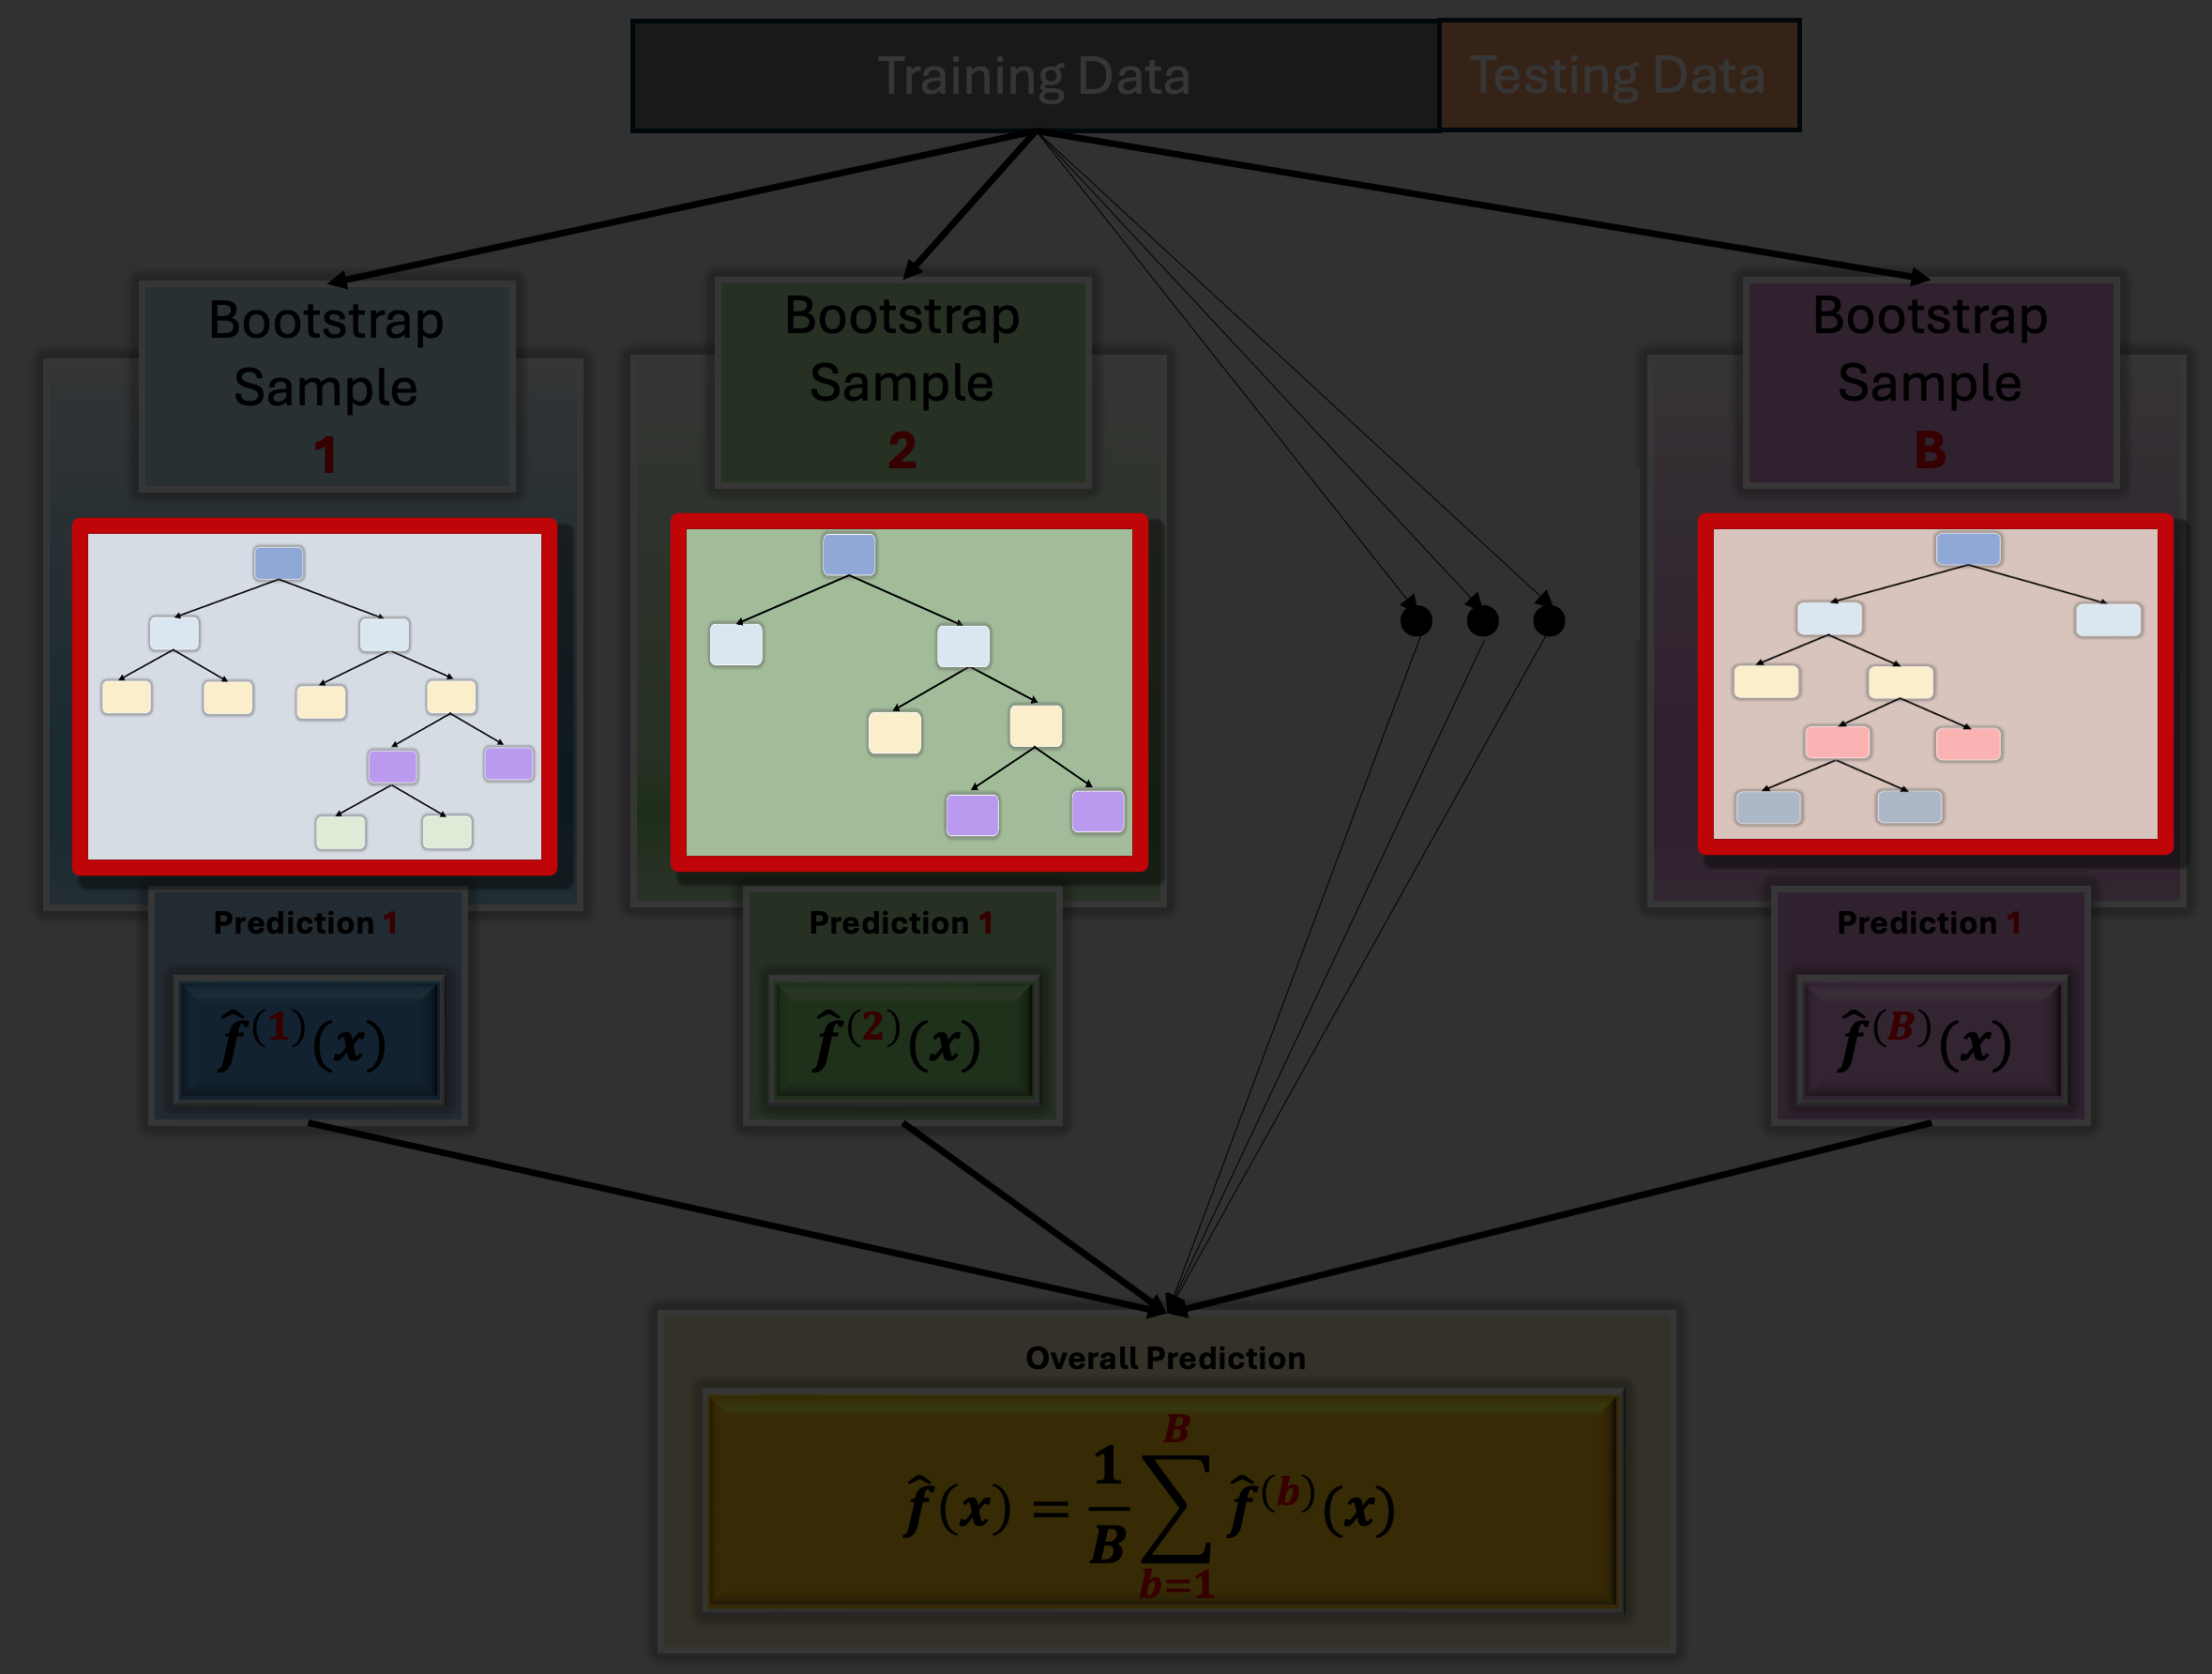
\includegraphics[scale=.24]{fig/Random_Forest_1.png}
\end{center}
}\\
\end{frame}



\begin{frame}\frametitle{Random Forest}
\qBrd[4.5in]{slateblue!50}{
\begin{center}
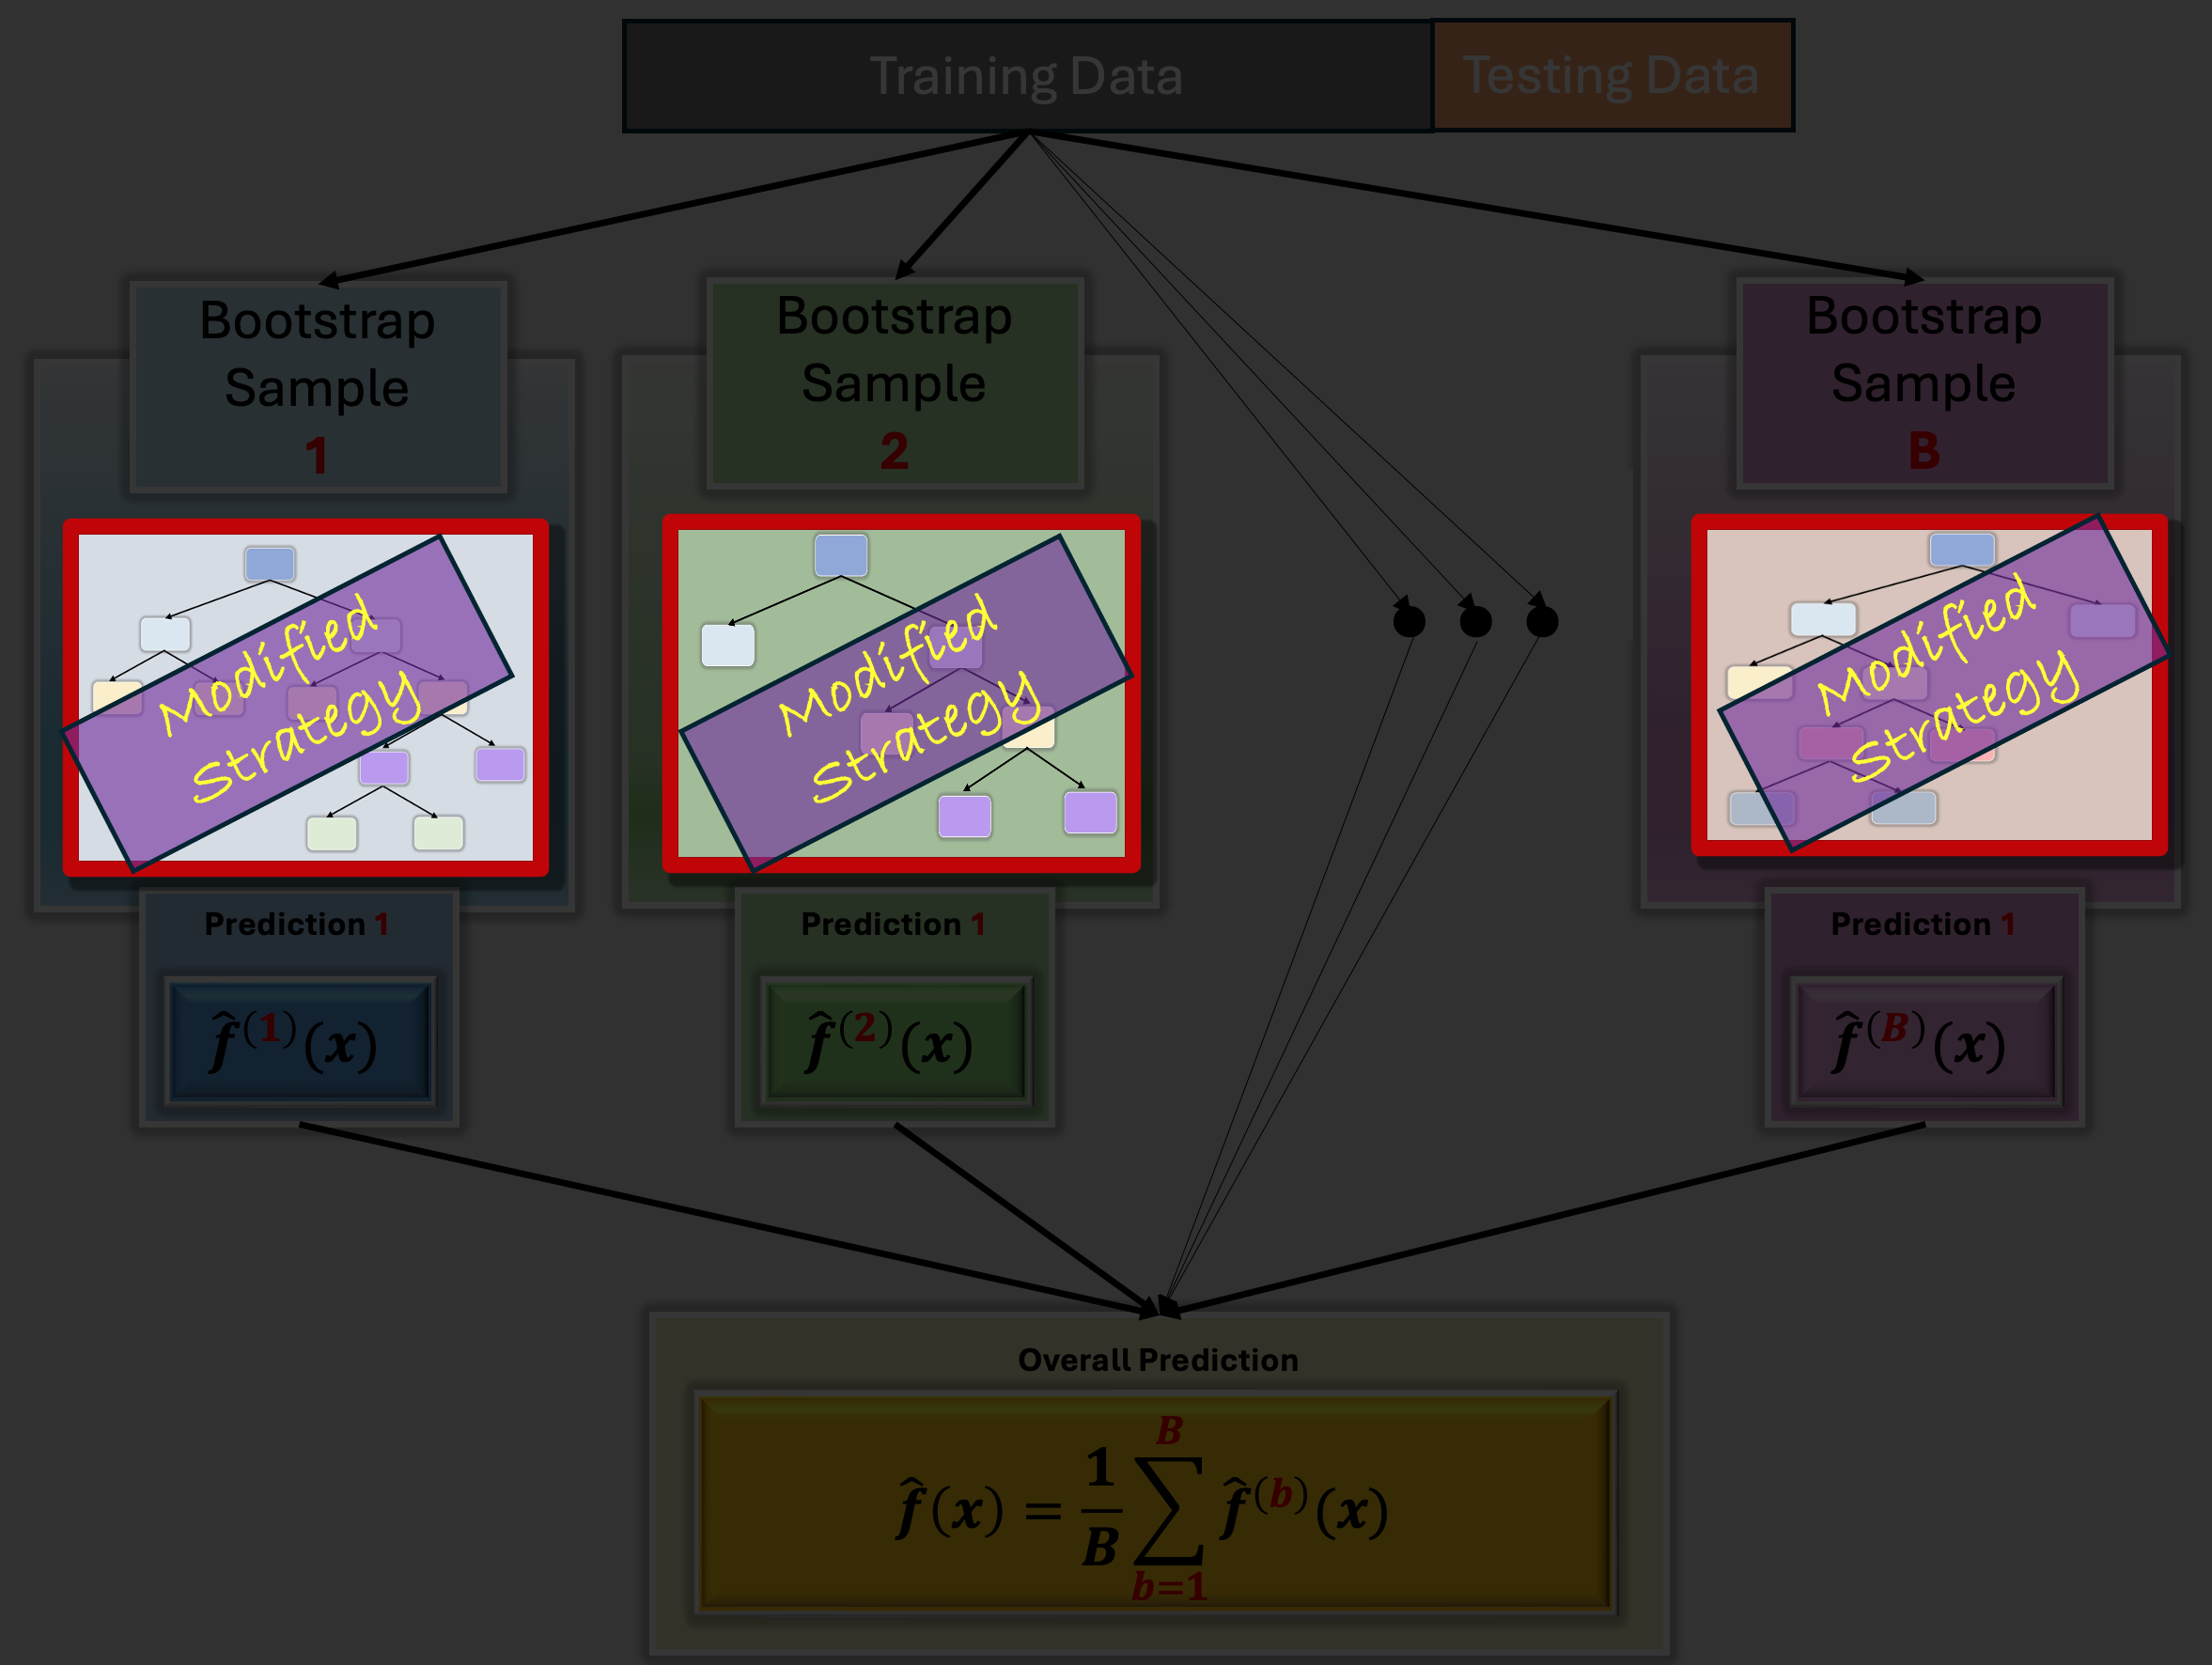
\includegraphics[scale=.24]{fig/Random_Forest_2.png}
\end{center}
}\\
\end{frame}

{
 \setbeamercolor{background canvas}{bg=}
\includepdf[pages={15}, scale=1]{STAT380-Unit4.pdf}
}


\begin{frame}\frametitle{Random Forest}
\qBrd[4.5in]{slateblue!50}{
\begin{center}
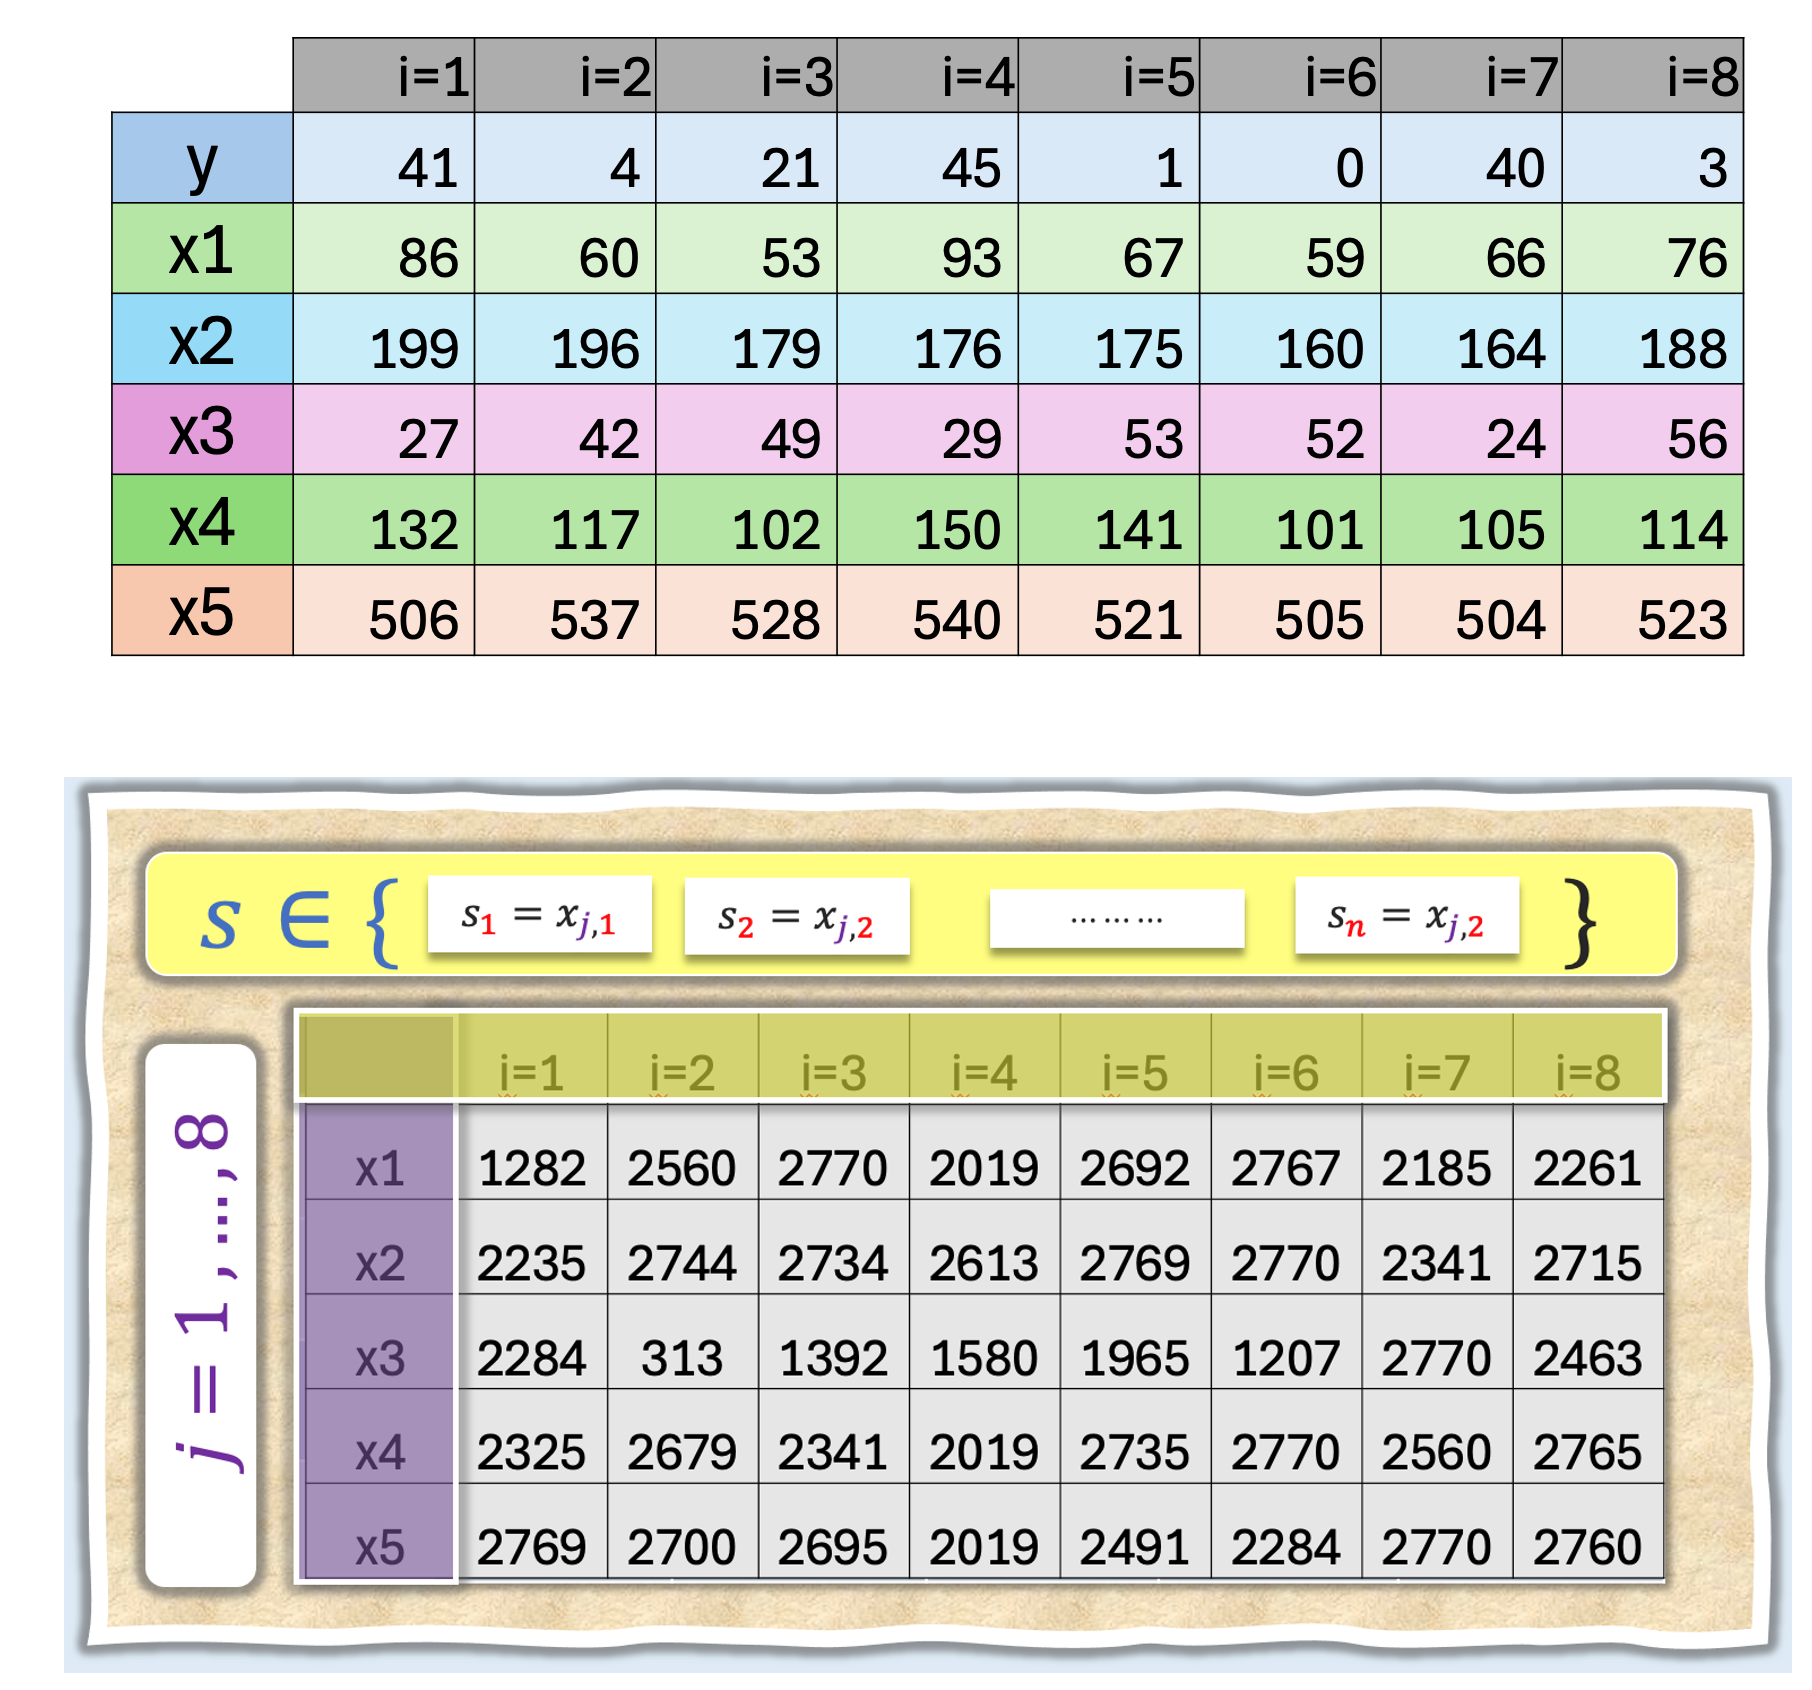
\includegraphics[scale=.24]{fig/Mock_Data_SSE_Table.png}
\end{center}
}\\
\end{frame}




\begin{frame}
\qBrd[4.7in]{babyblueeyes!50}{
\begin{center}
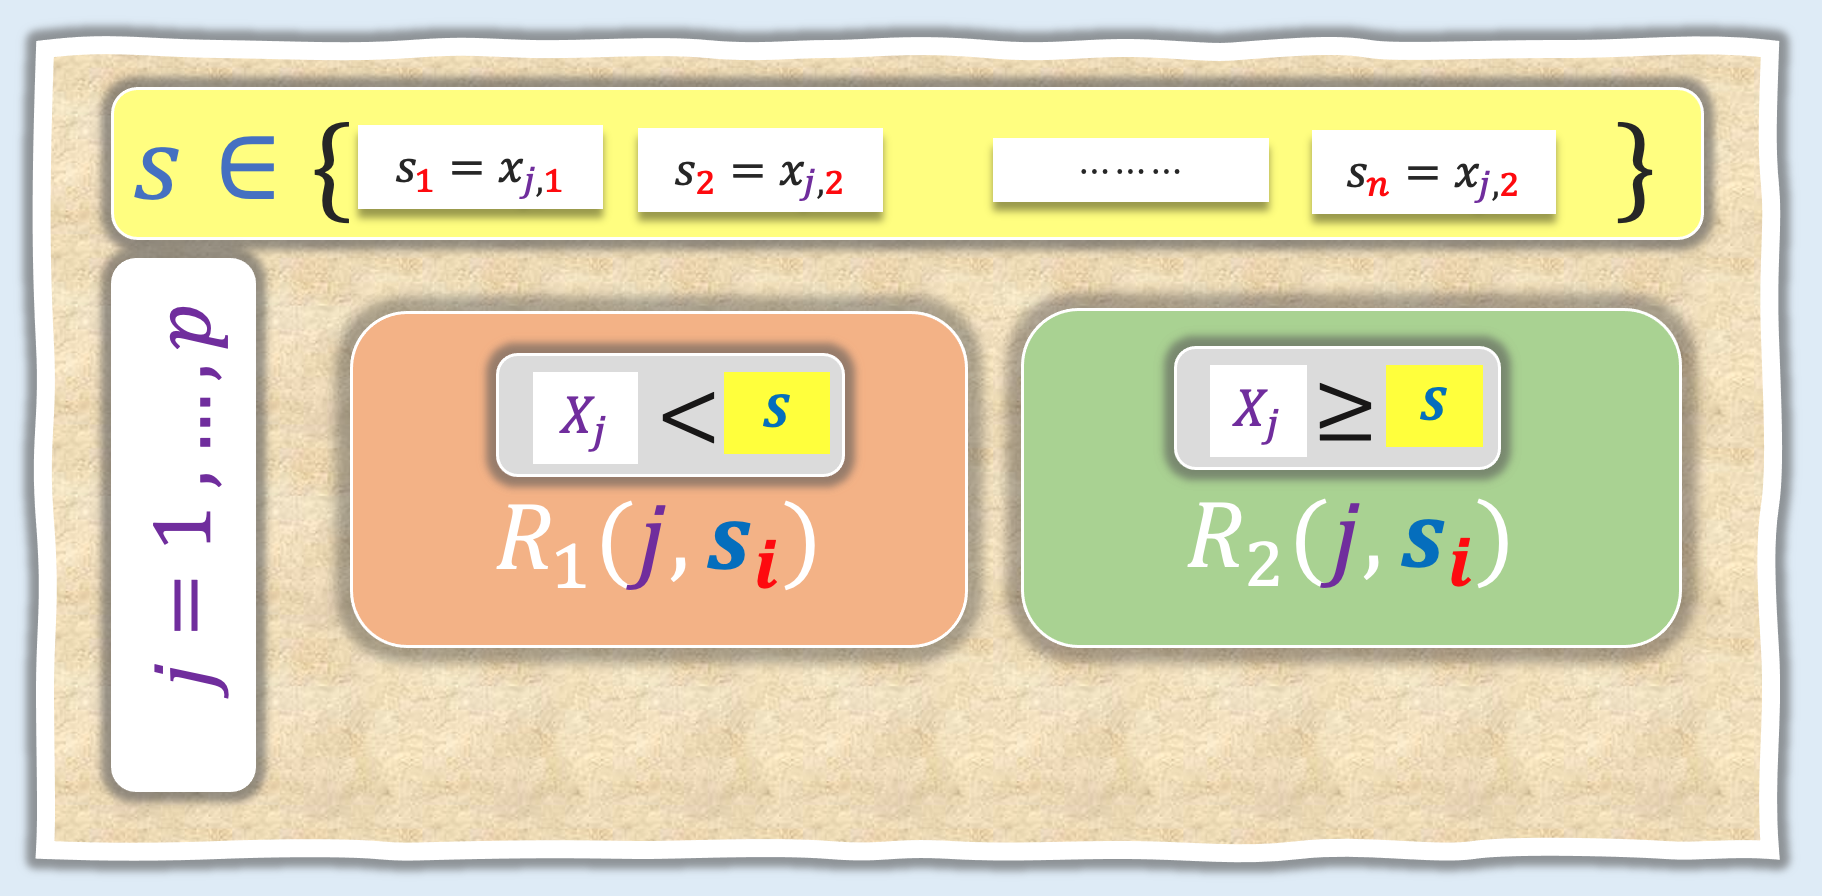
\includegraphics[scale=.35]{figs/R1_R2_s.png}
\end{center}
%\vspace{.1in}
}\\
\qBrd[4.7in]{airforceblue!50}{$$\HLTW{ \text{C}(j, s_i)}:=  {\HLTW{ \displaystyle  \sum_{\HLTEQ[rose!40]{i\in \HLTY{ R_1(j, s_i)}}}^{}\left(y_i - \HLTY{ \widehat{y}_{_{R_1}}} \right)^2  } + \HLTW{ \displaystyle  \sum_{ \HLTEQ[rose!40]{i\in \HLTY{ R_2(j, s_i)}}}^{}\left(y_i - \HLTY{ \widehat{y}_{_{R_2}}} \right)^2  }}$$
}

\end{frame}


\begin{frame}\frametitle{Random Forest}
\qBrd[4.5in]{slateblue!50}{
\begin{center}
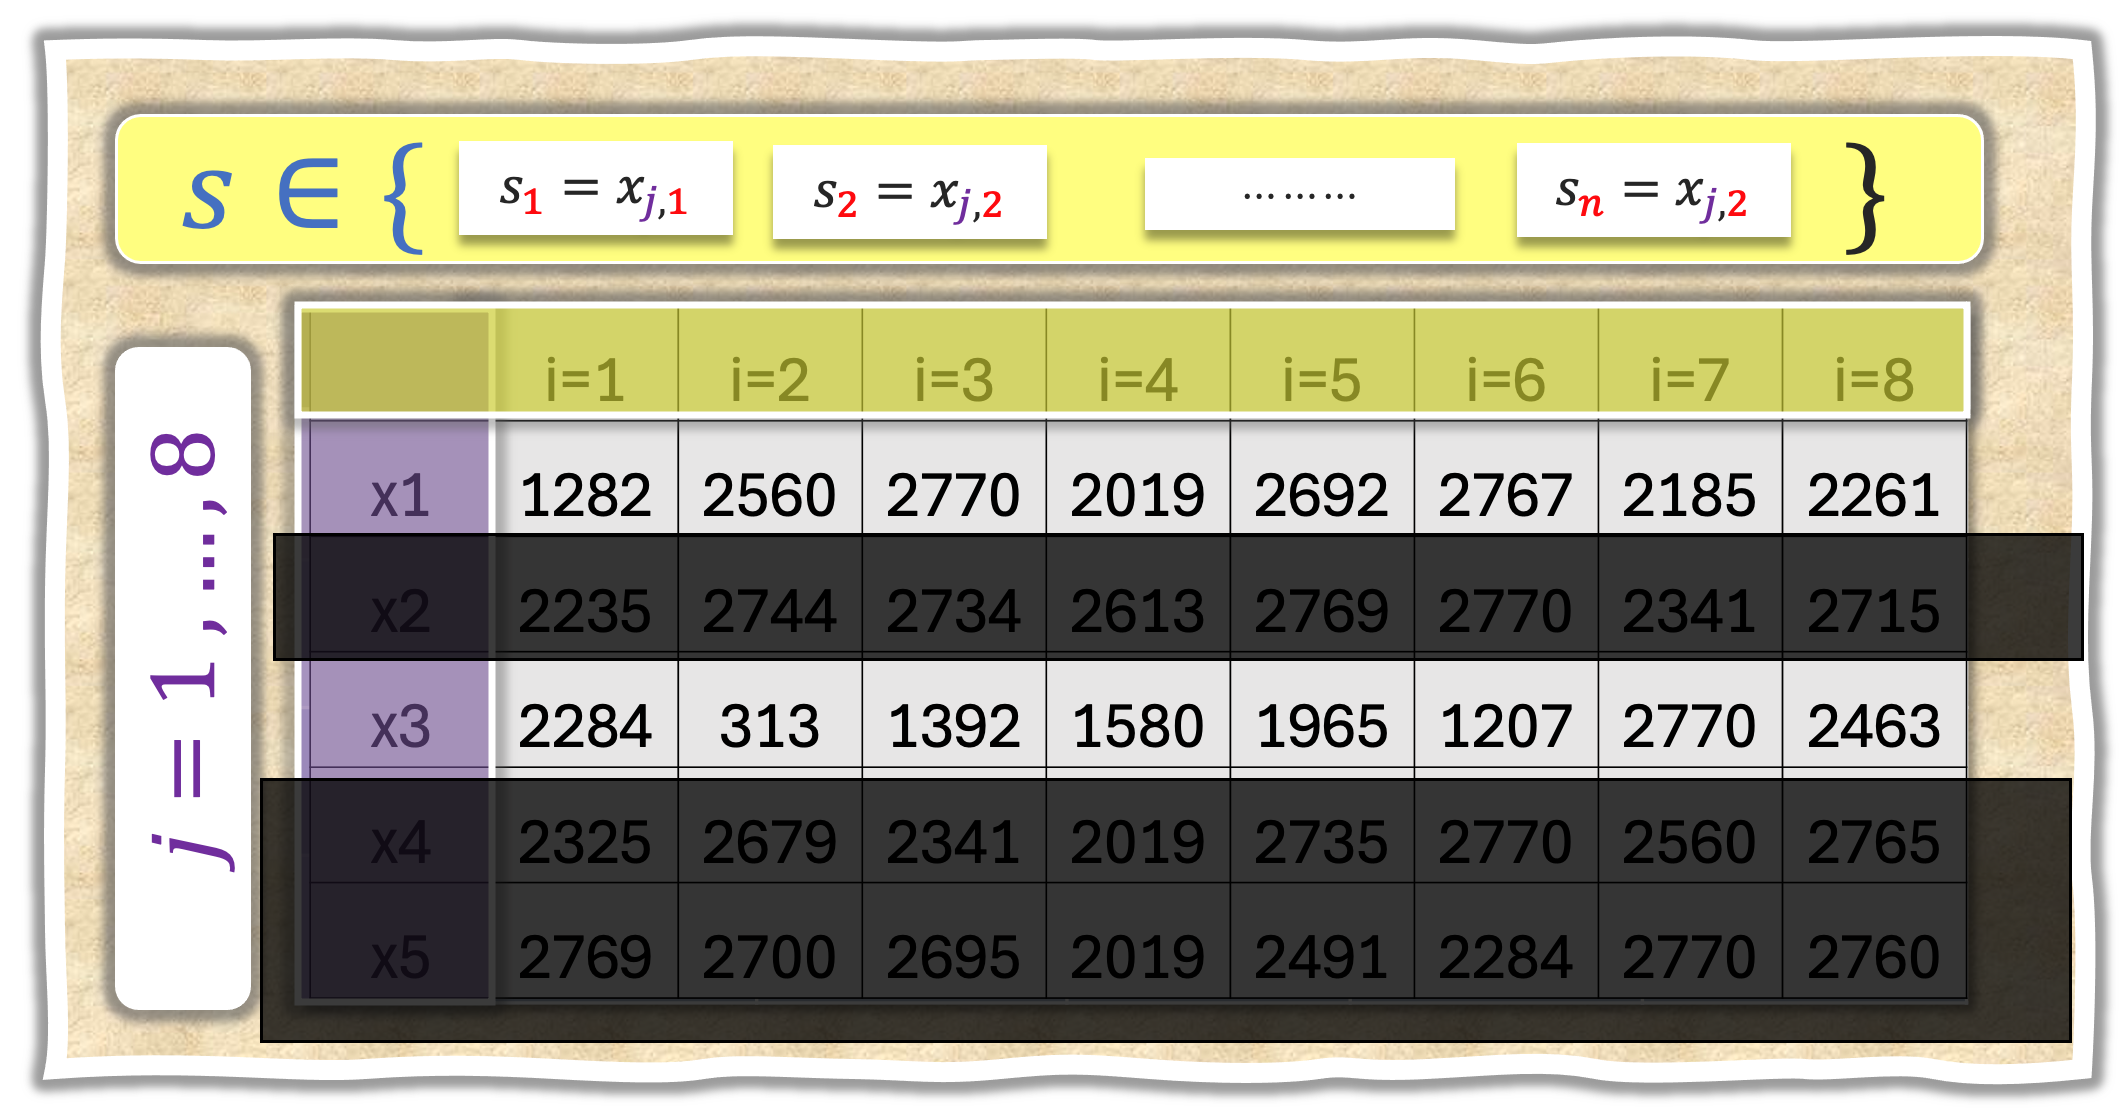
\includegraphics[scale=.24]{fig/Bootstrap_Updated_Table1.png}
\qBrd[2.5in]{olive!50}{ The randomly selected variables to be considered are  $X_1, X_3$.}
\end{center}
}\\
\end{frame}




\begin{frame}\frametitle{Random Forest}
\qBrd[4.5in]{slateblue!50}{
\begin{center}
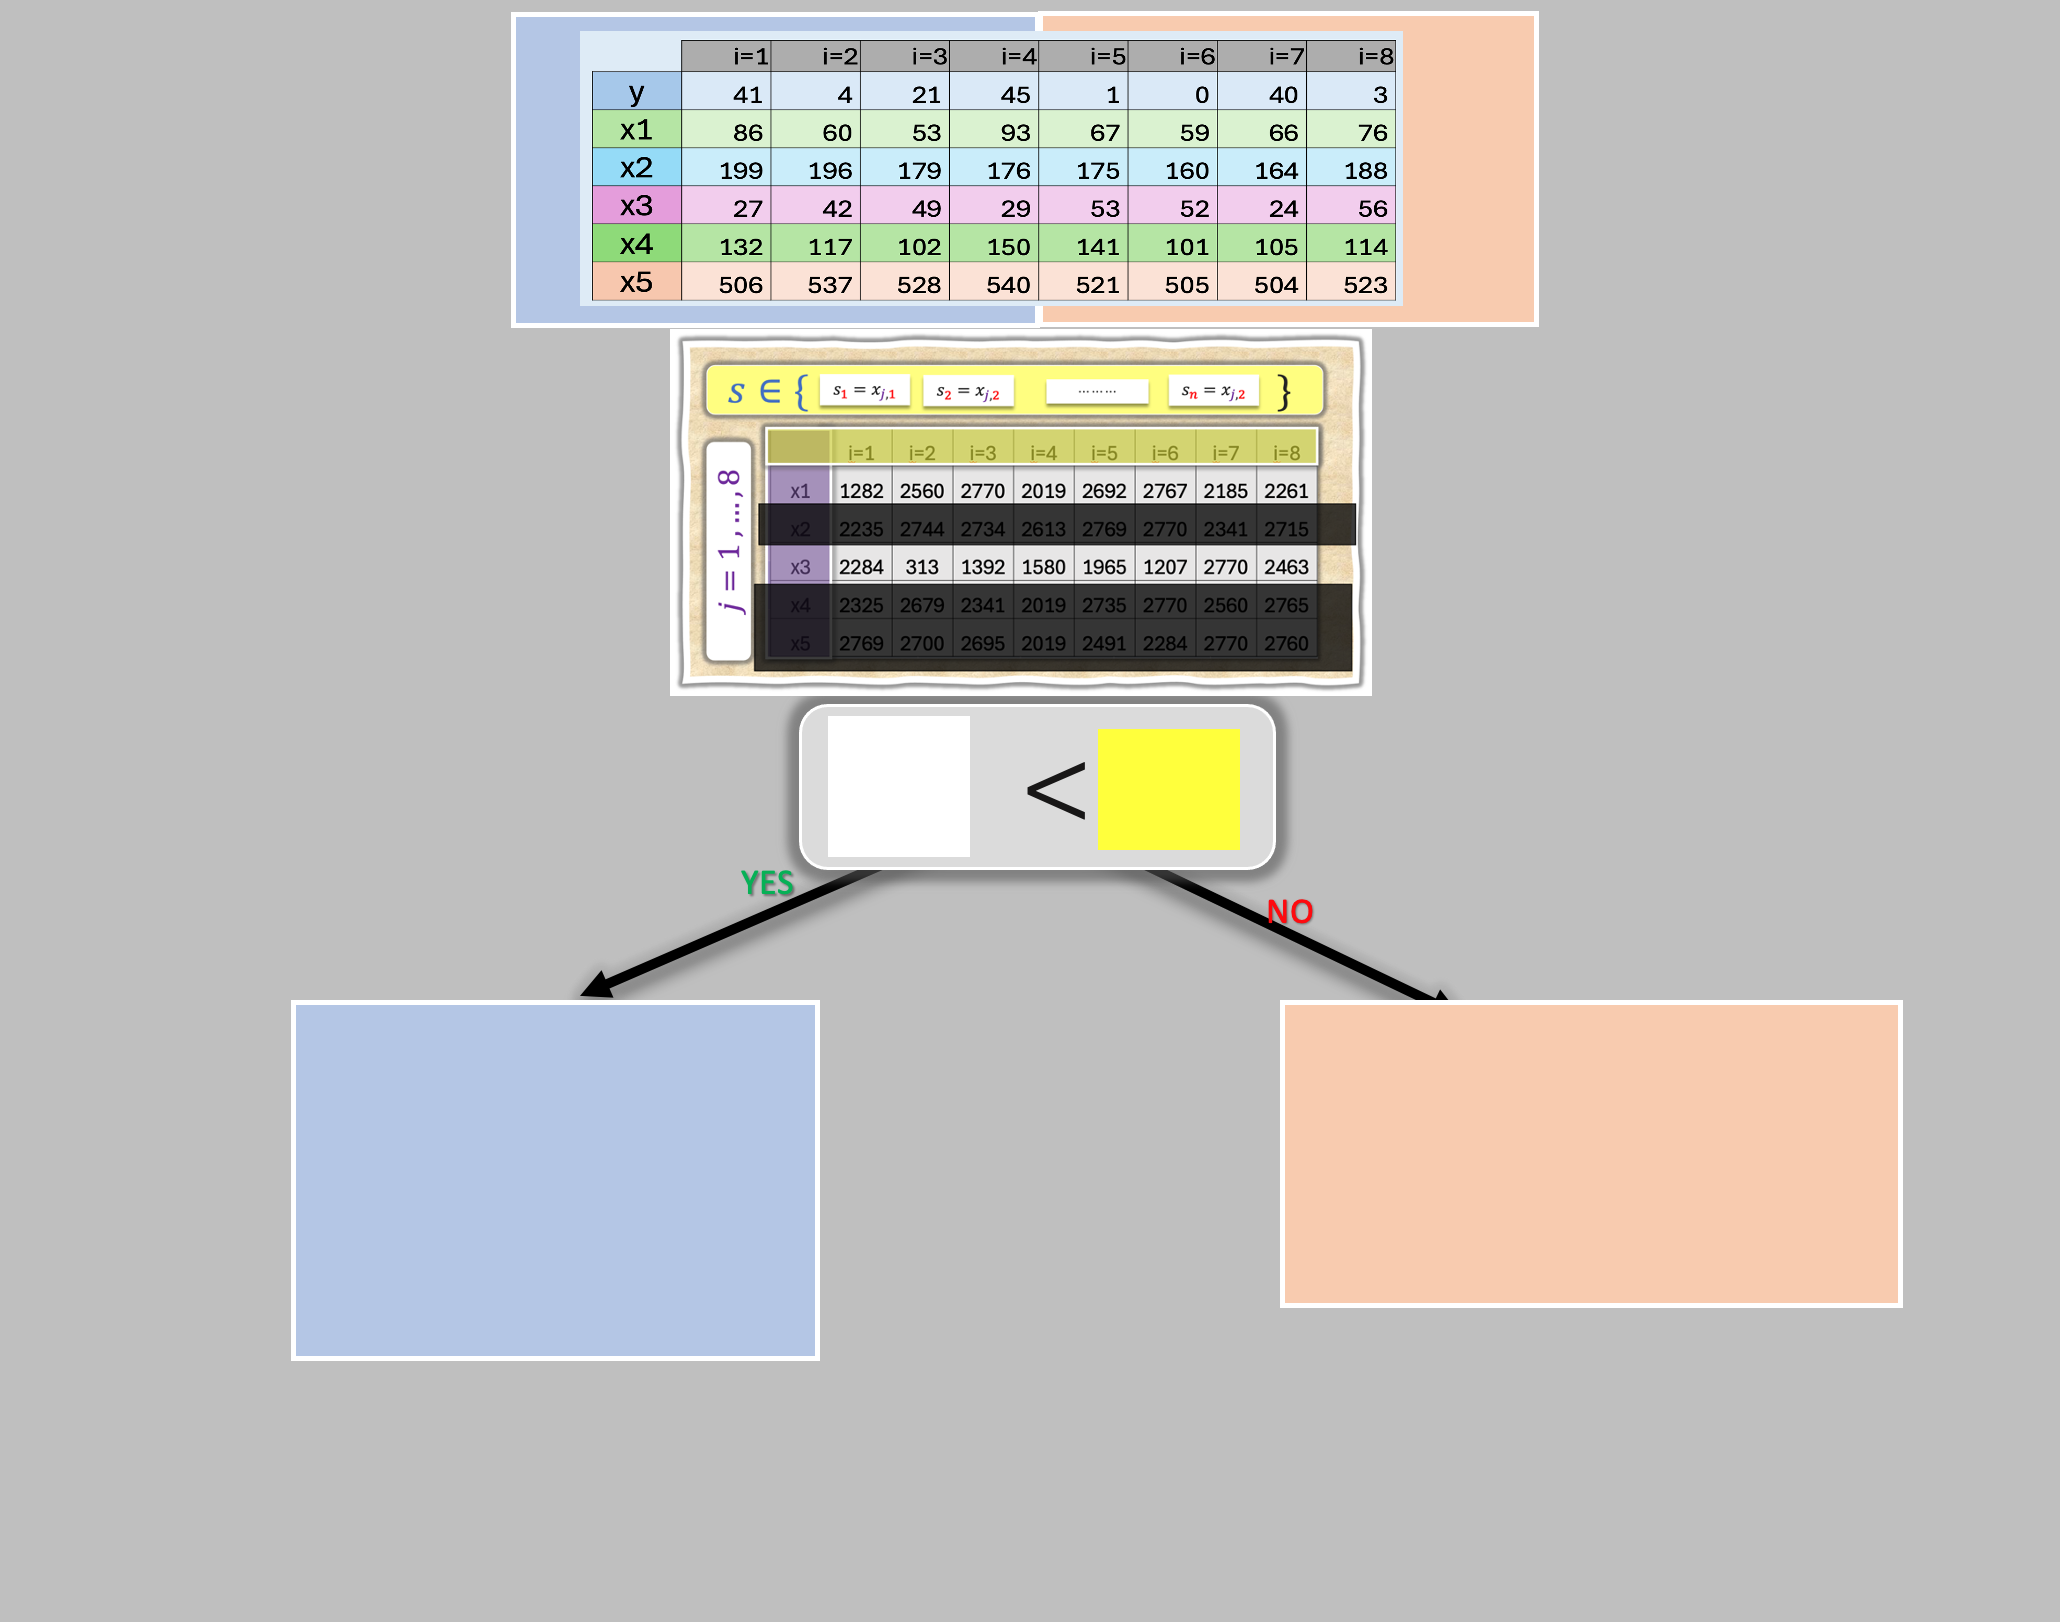
\includegraphics[scale=.24]{fig/RF_TOY_DATA_Step1.png}
\end{center}
}\\
\end{frame}



\begin{frame}\frametitle{Random Forest}
\qBrd[4.5in]{slateblue!50}{
\begin{center}
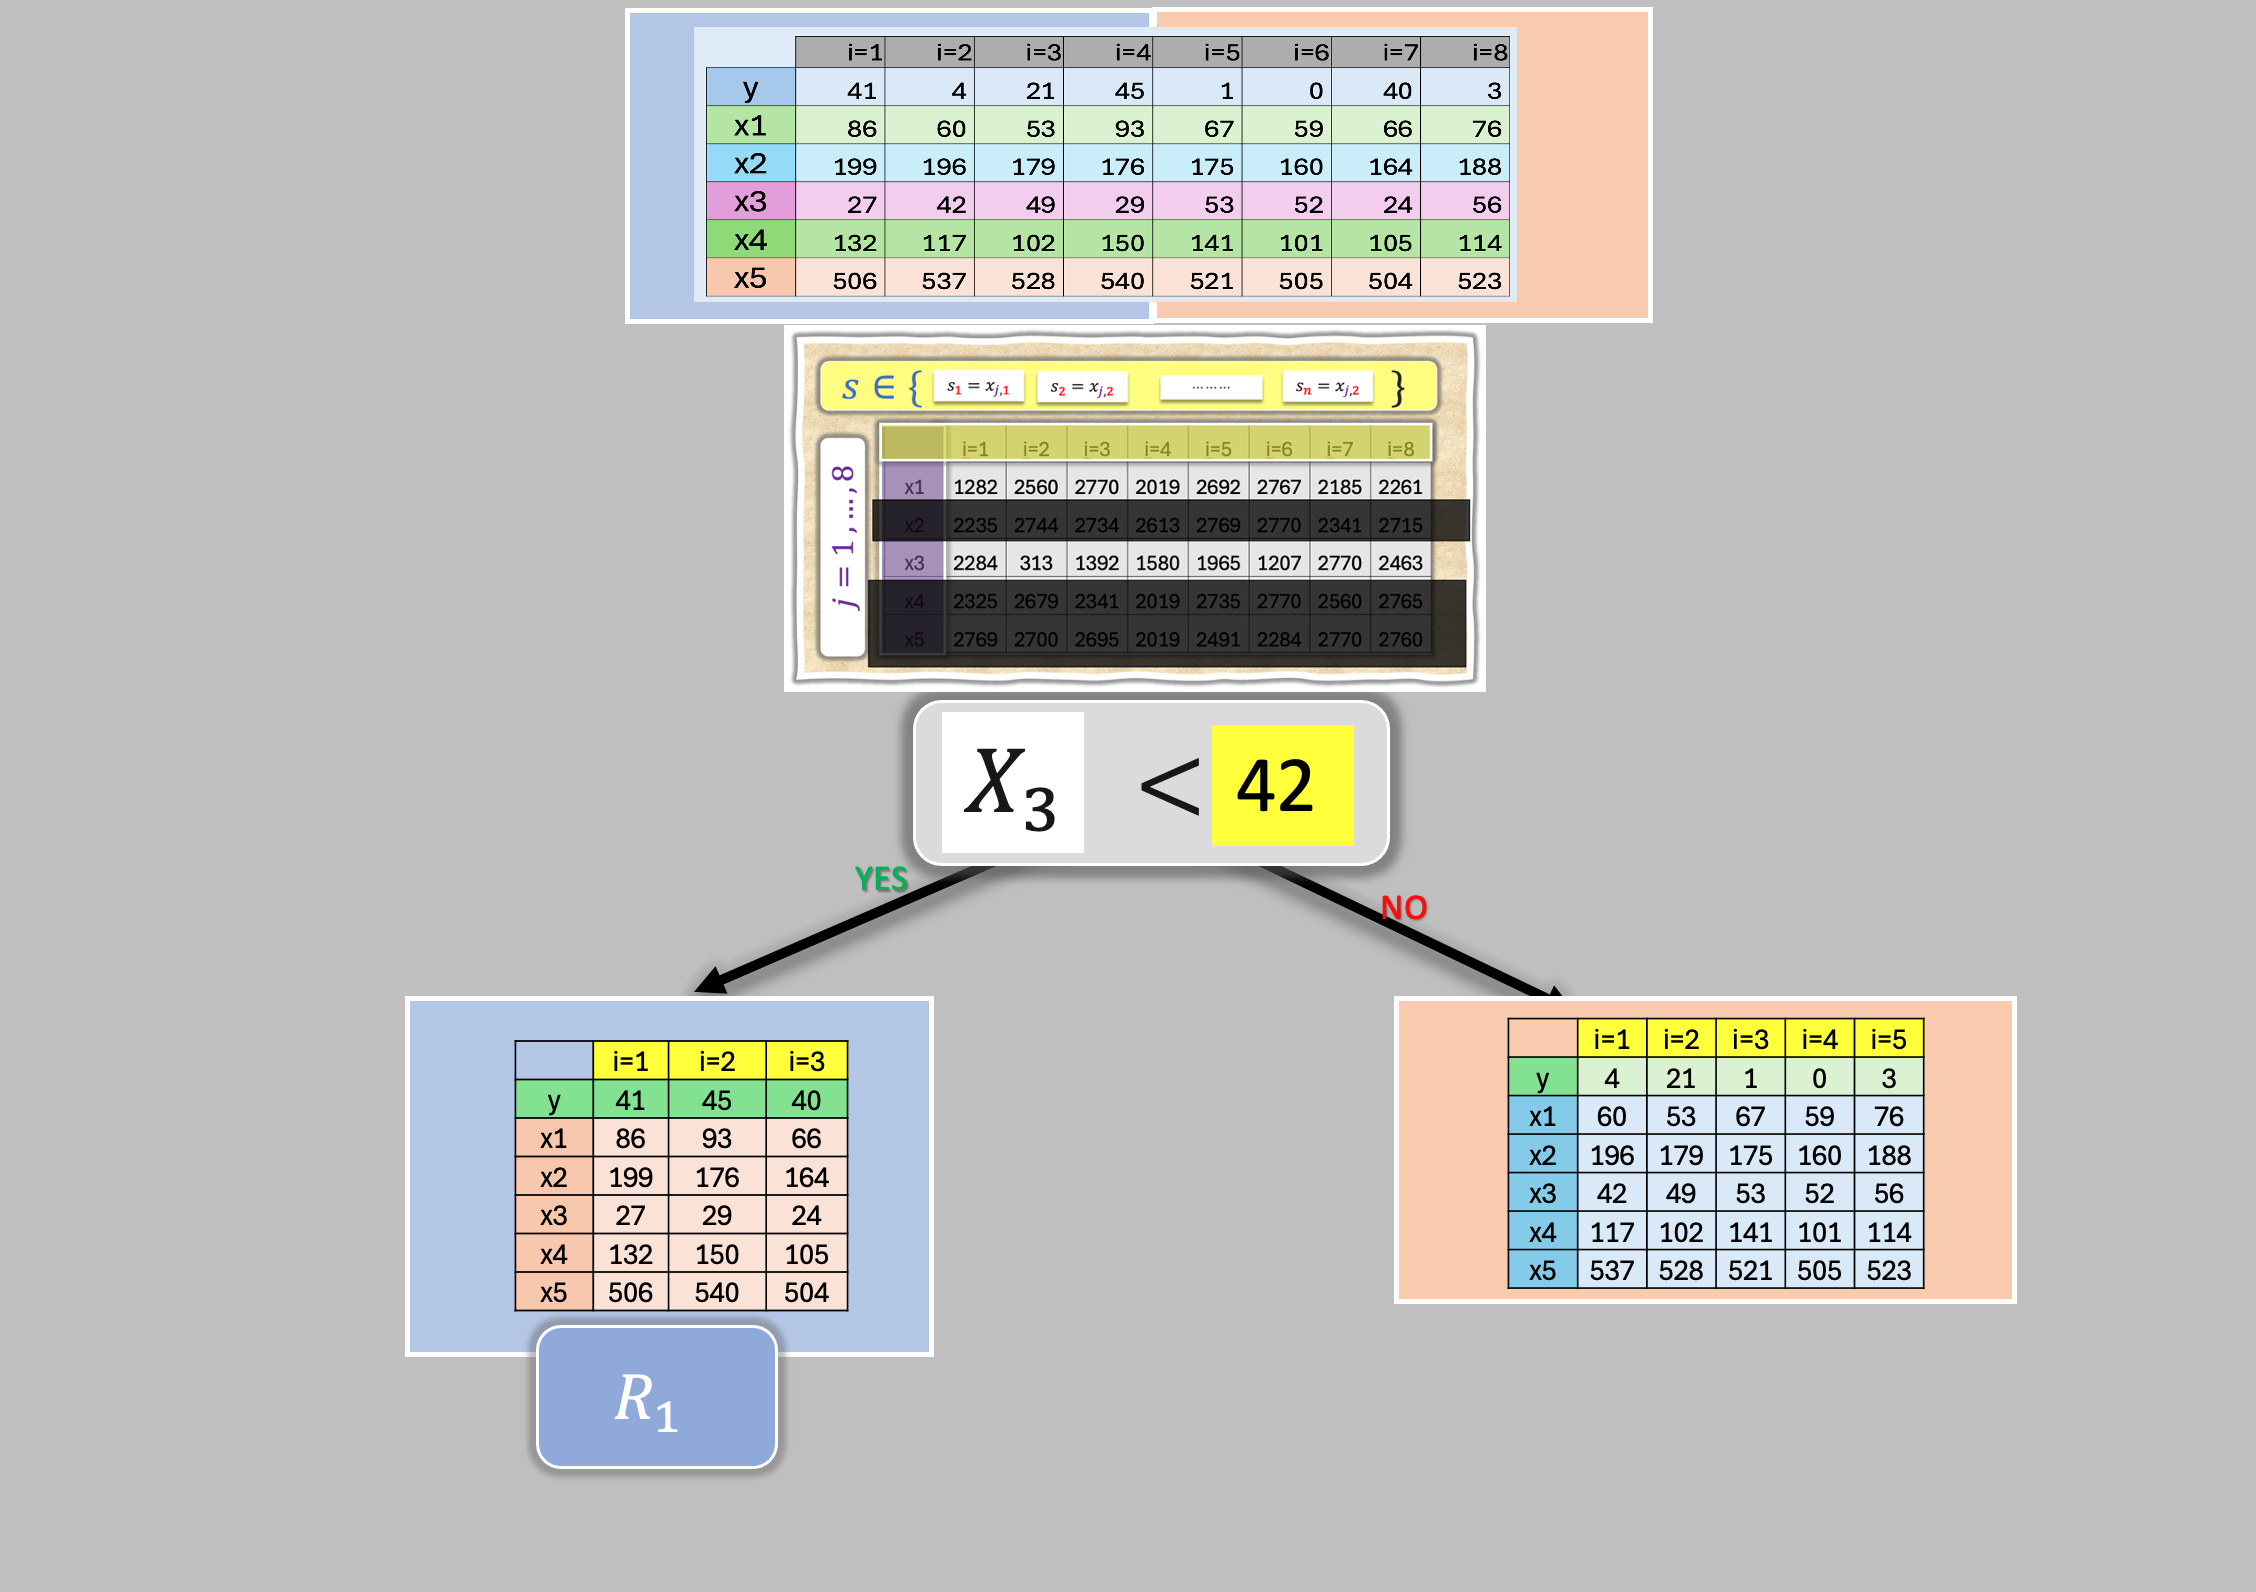
\includegraphics[scale=.24]{fig/RF_TOY_DATA_Step2.png}
\end{center}
}\\
\end{frame}




\begin{frame}\frametitle{Random Forest}
\qBrd[4.5in]{slateblue!50}{
\begin{center}
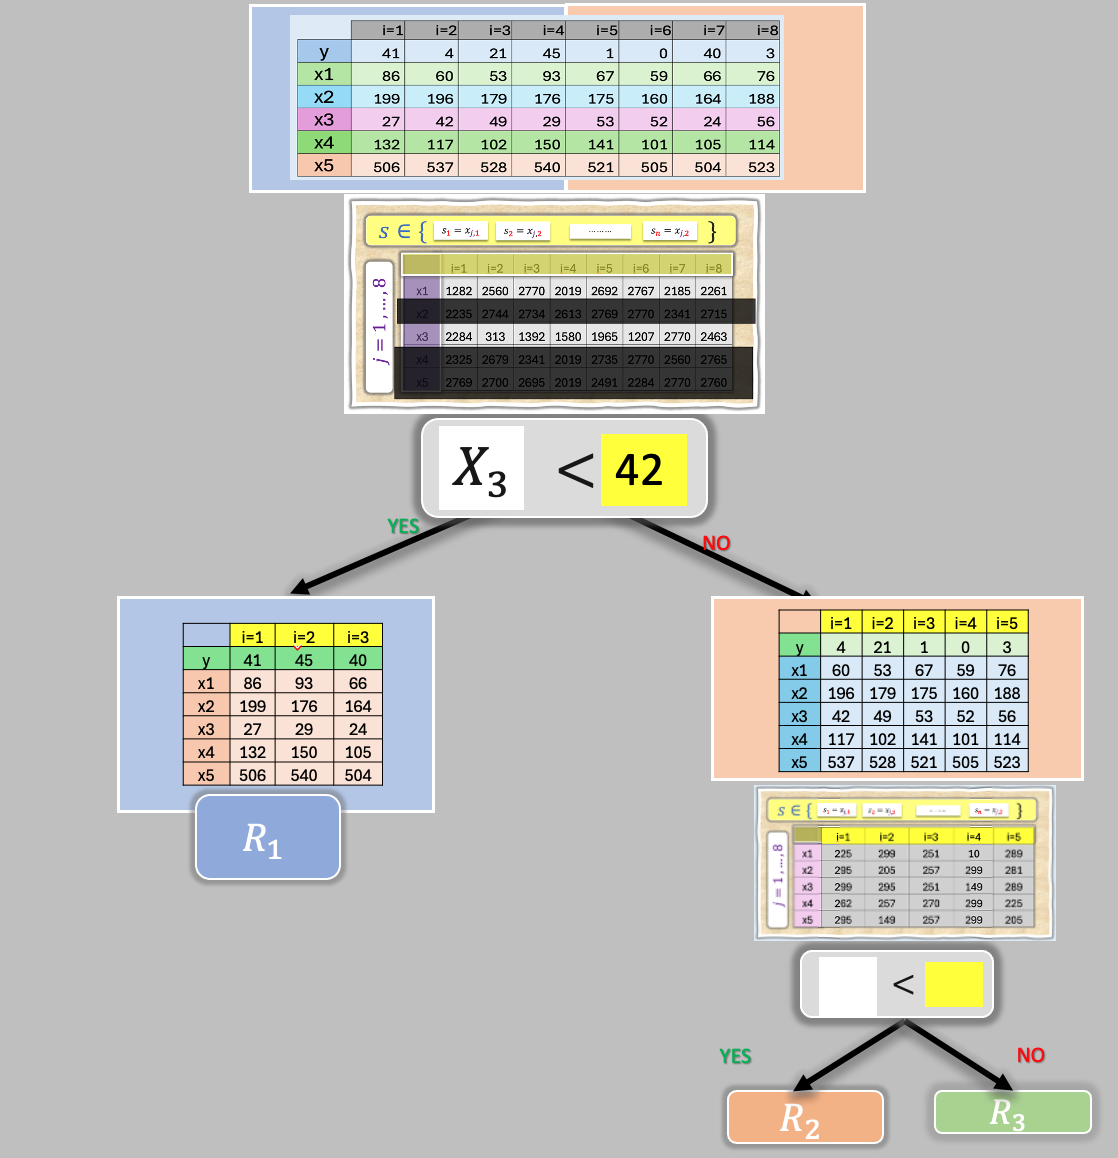
\includegraphics[scale=.38]{fig/RF_TOY_DATA_Step3.png}
\end{center}
}\\
\end{frame}



\begin{frame}\frametitle{Standard Strategy \& Random Forest}
\qBrd[4.5in]{slateblue!50}{
\begin{center}
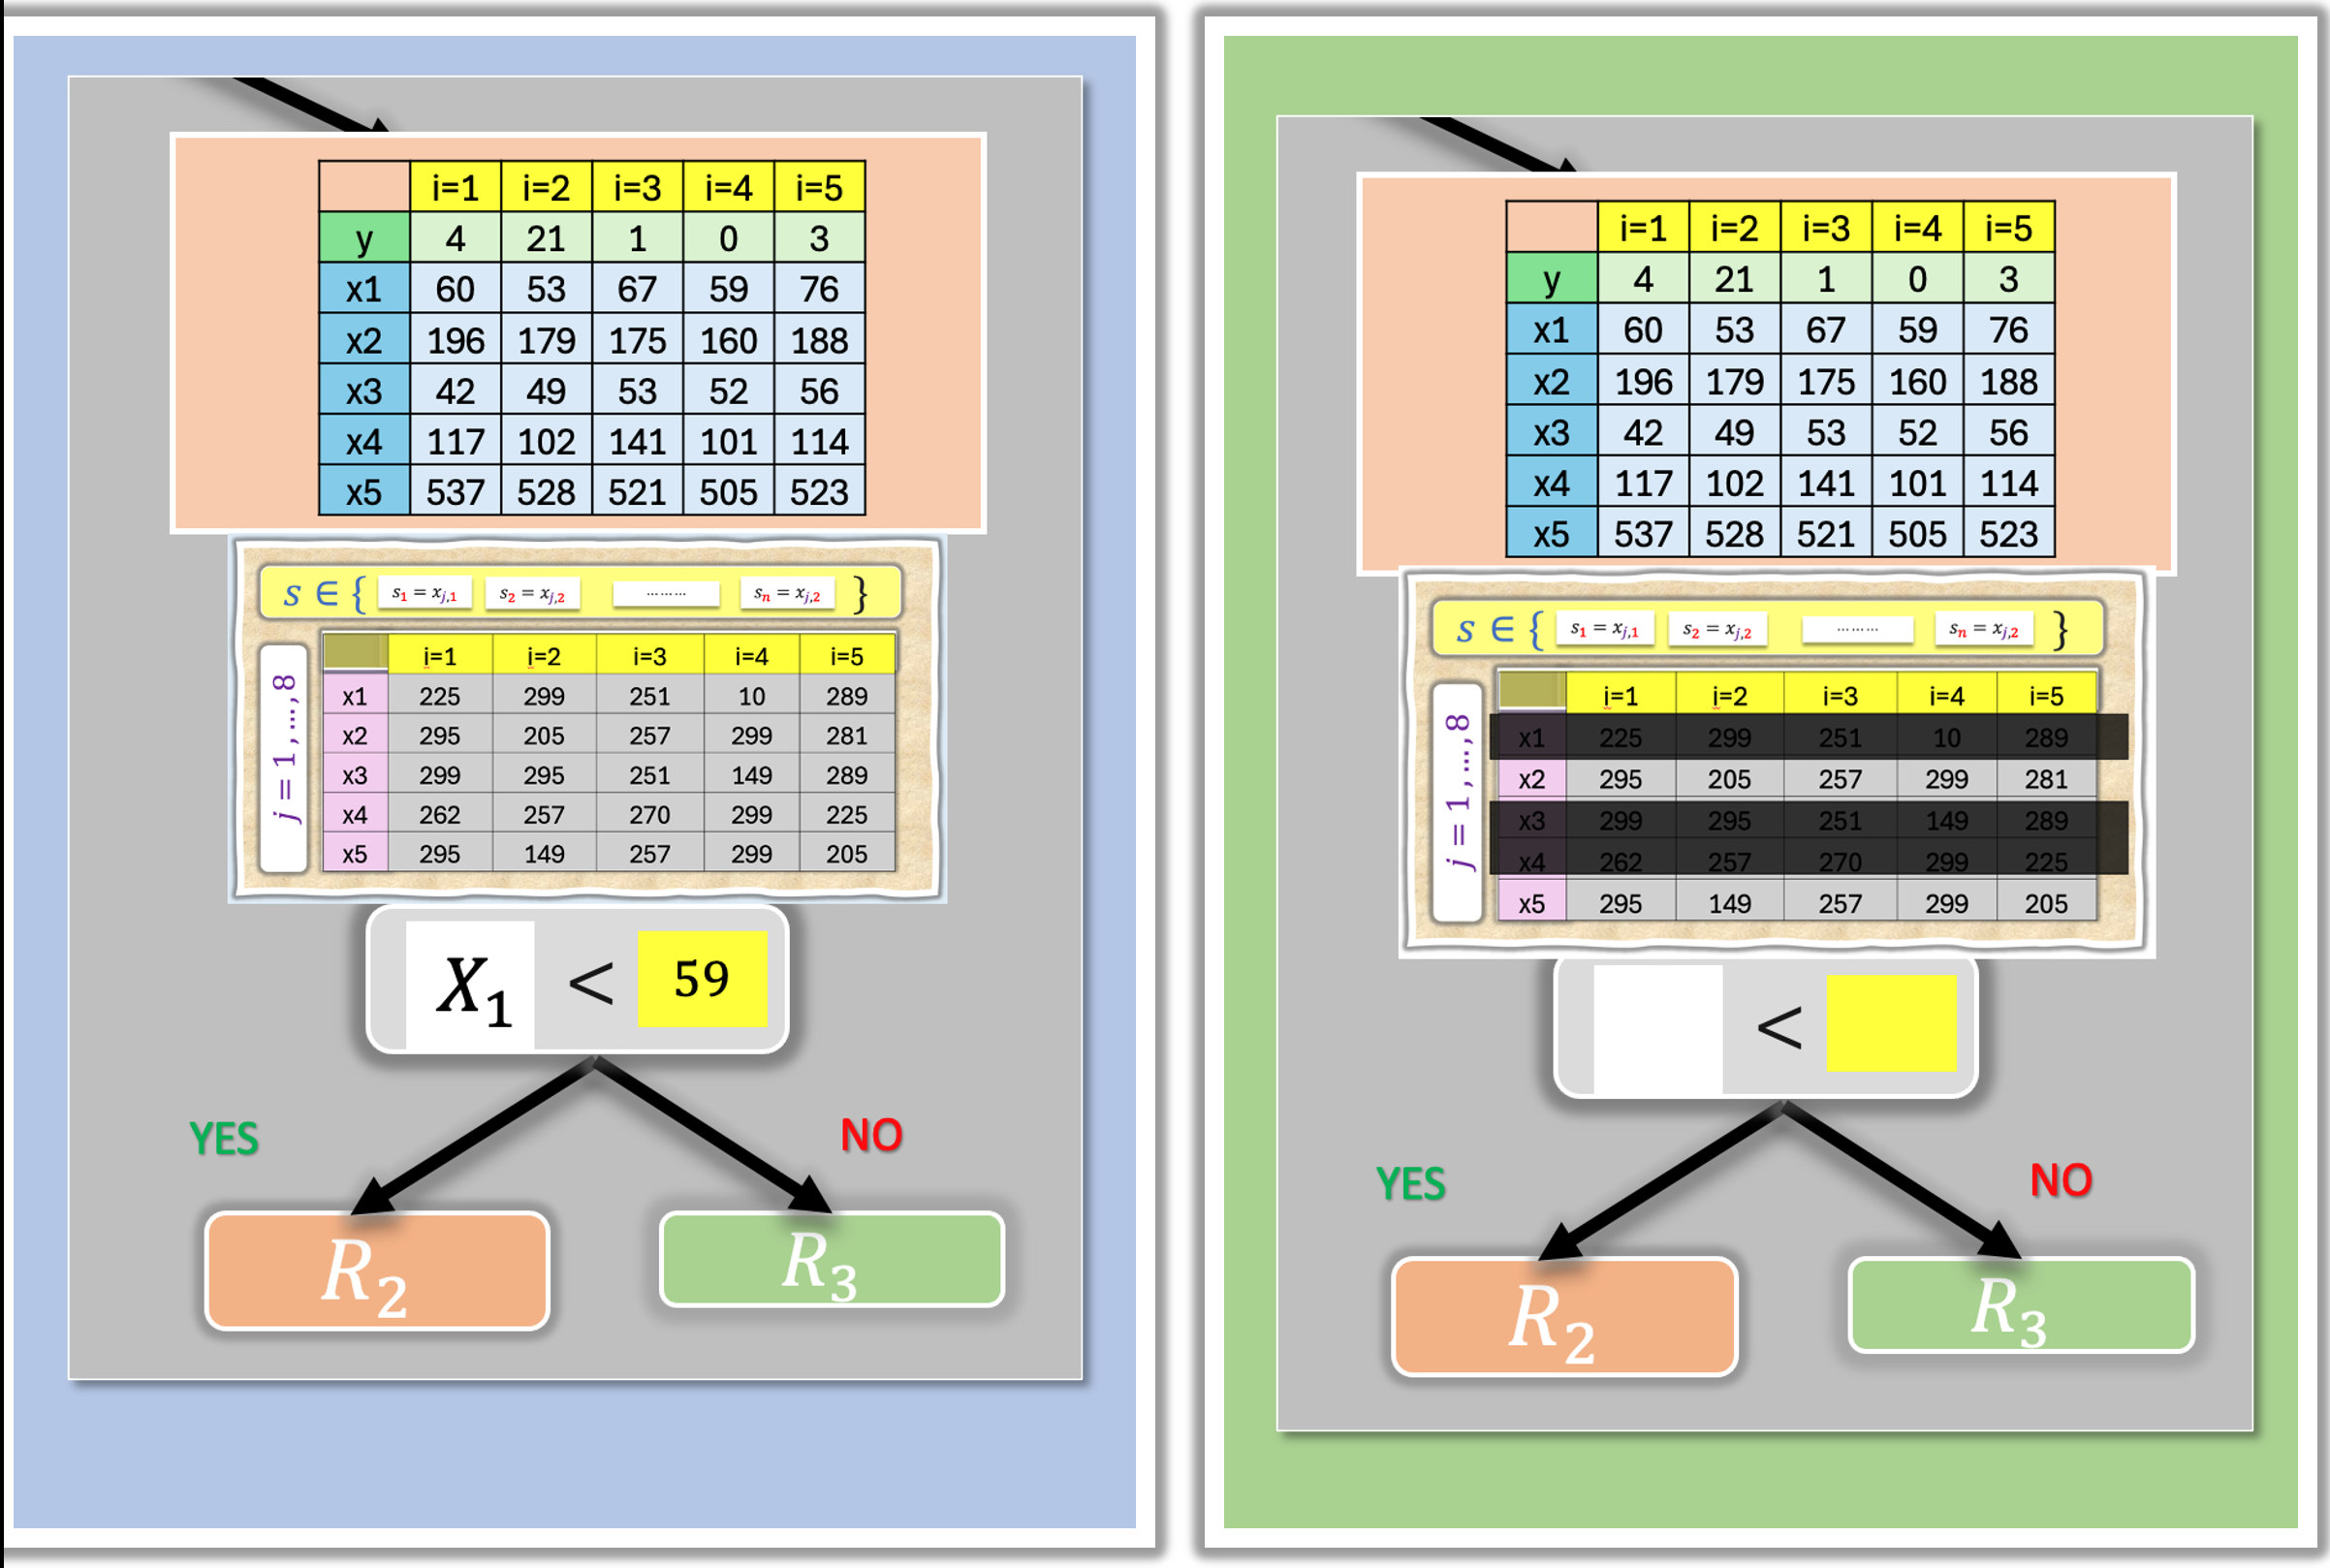
\includegraphics[scale=.25]{fig/RF_TOY_DATA_Two_Strategy.png}
\qBrd[2.5in]{applegreen!50}{ \tiny The randomly selected variables to be considered are  $X_1, X_3$.}
\end{center}
}\\
\end{frame}





\begin{frame}\frametitle{Random Forest}
\qBrd[4.5in]{slateblue!50}{
\begin{center}
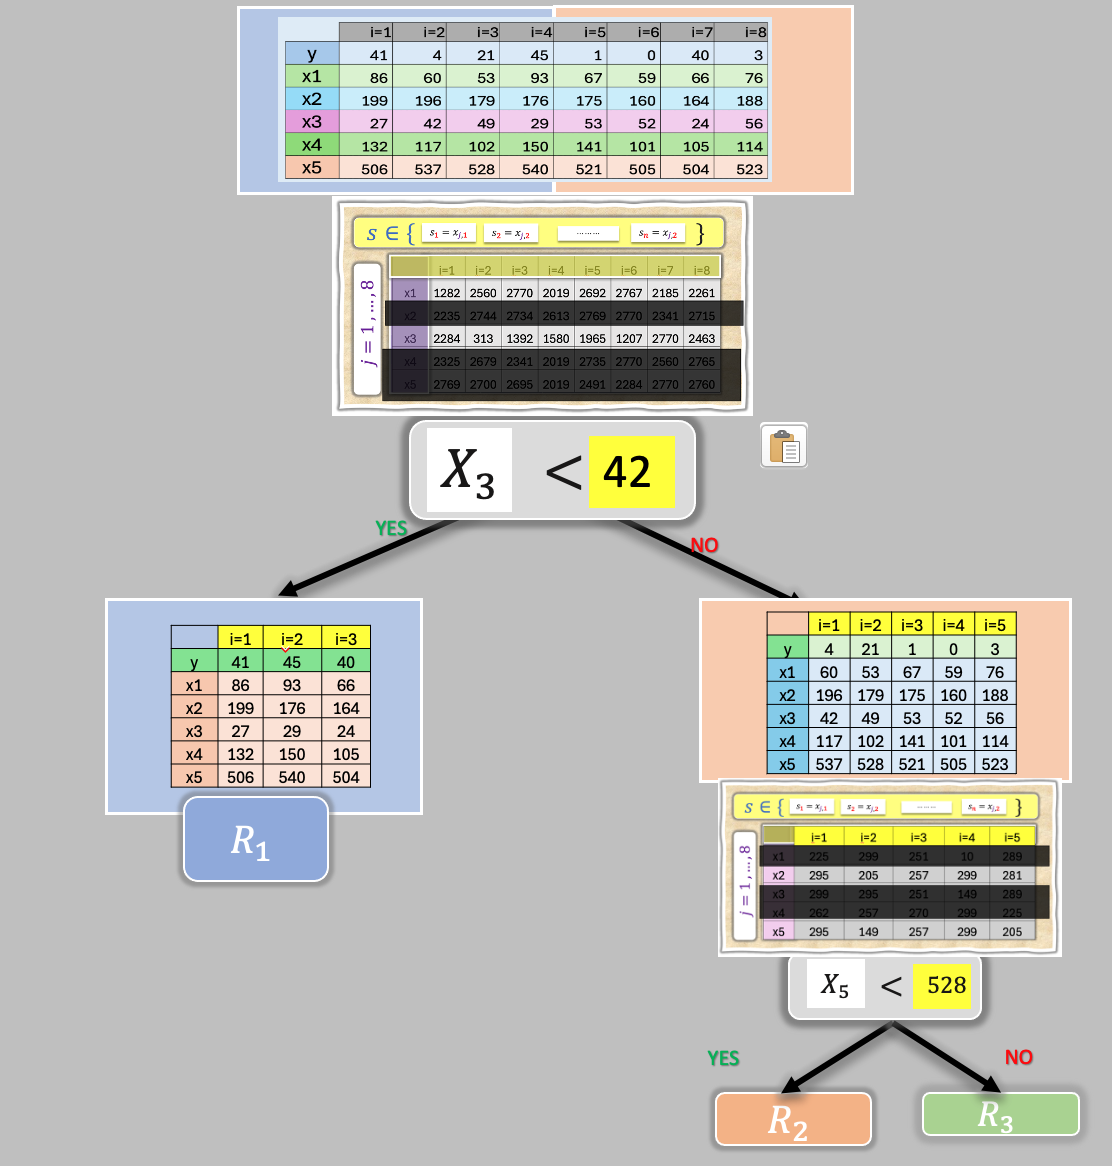
\includegraphics[scale=.38]{fig/RF_TOY_DATA_Step4.png}
\end{center}
}\\
\end{frame}





\begin{frame}\frametitle{Random Forest}
\qBrd[4.5in]{slateblue!50}{
\begin{center}
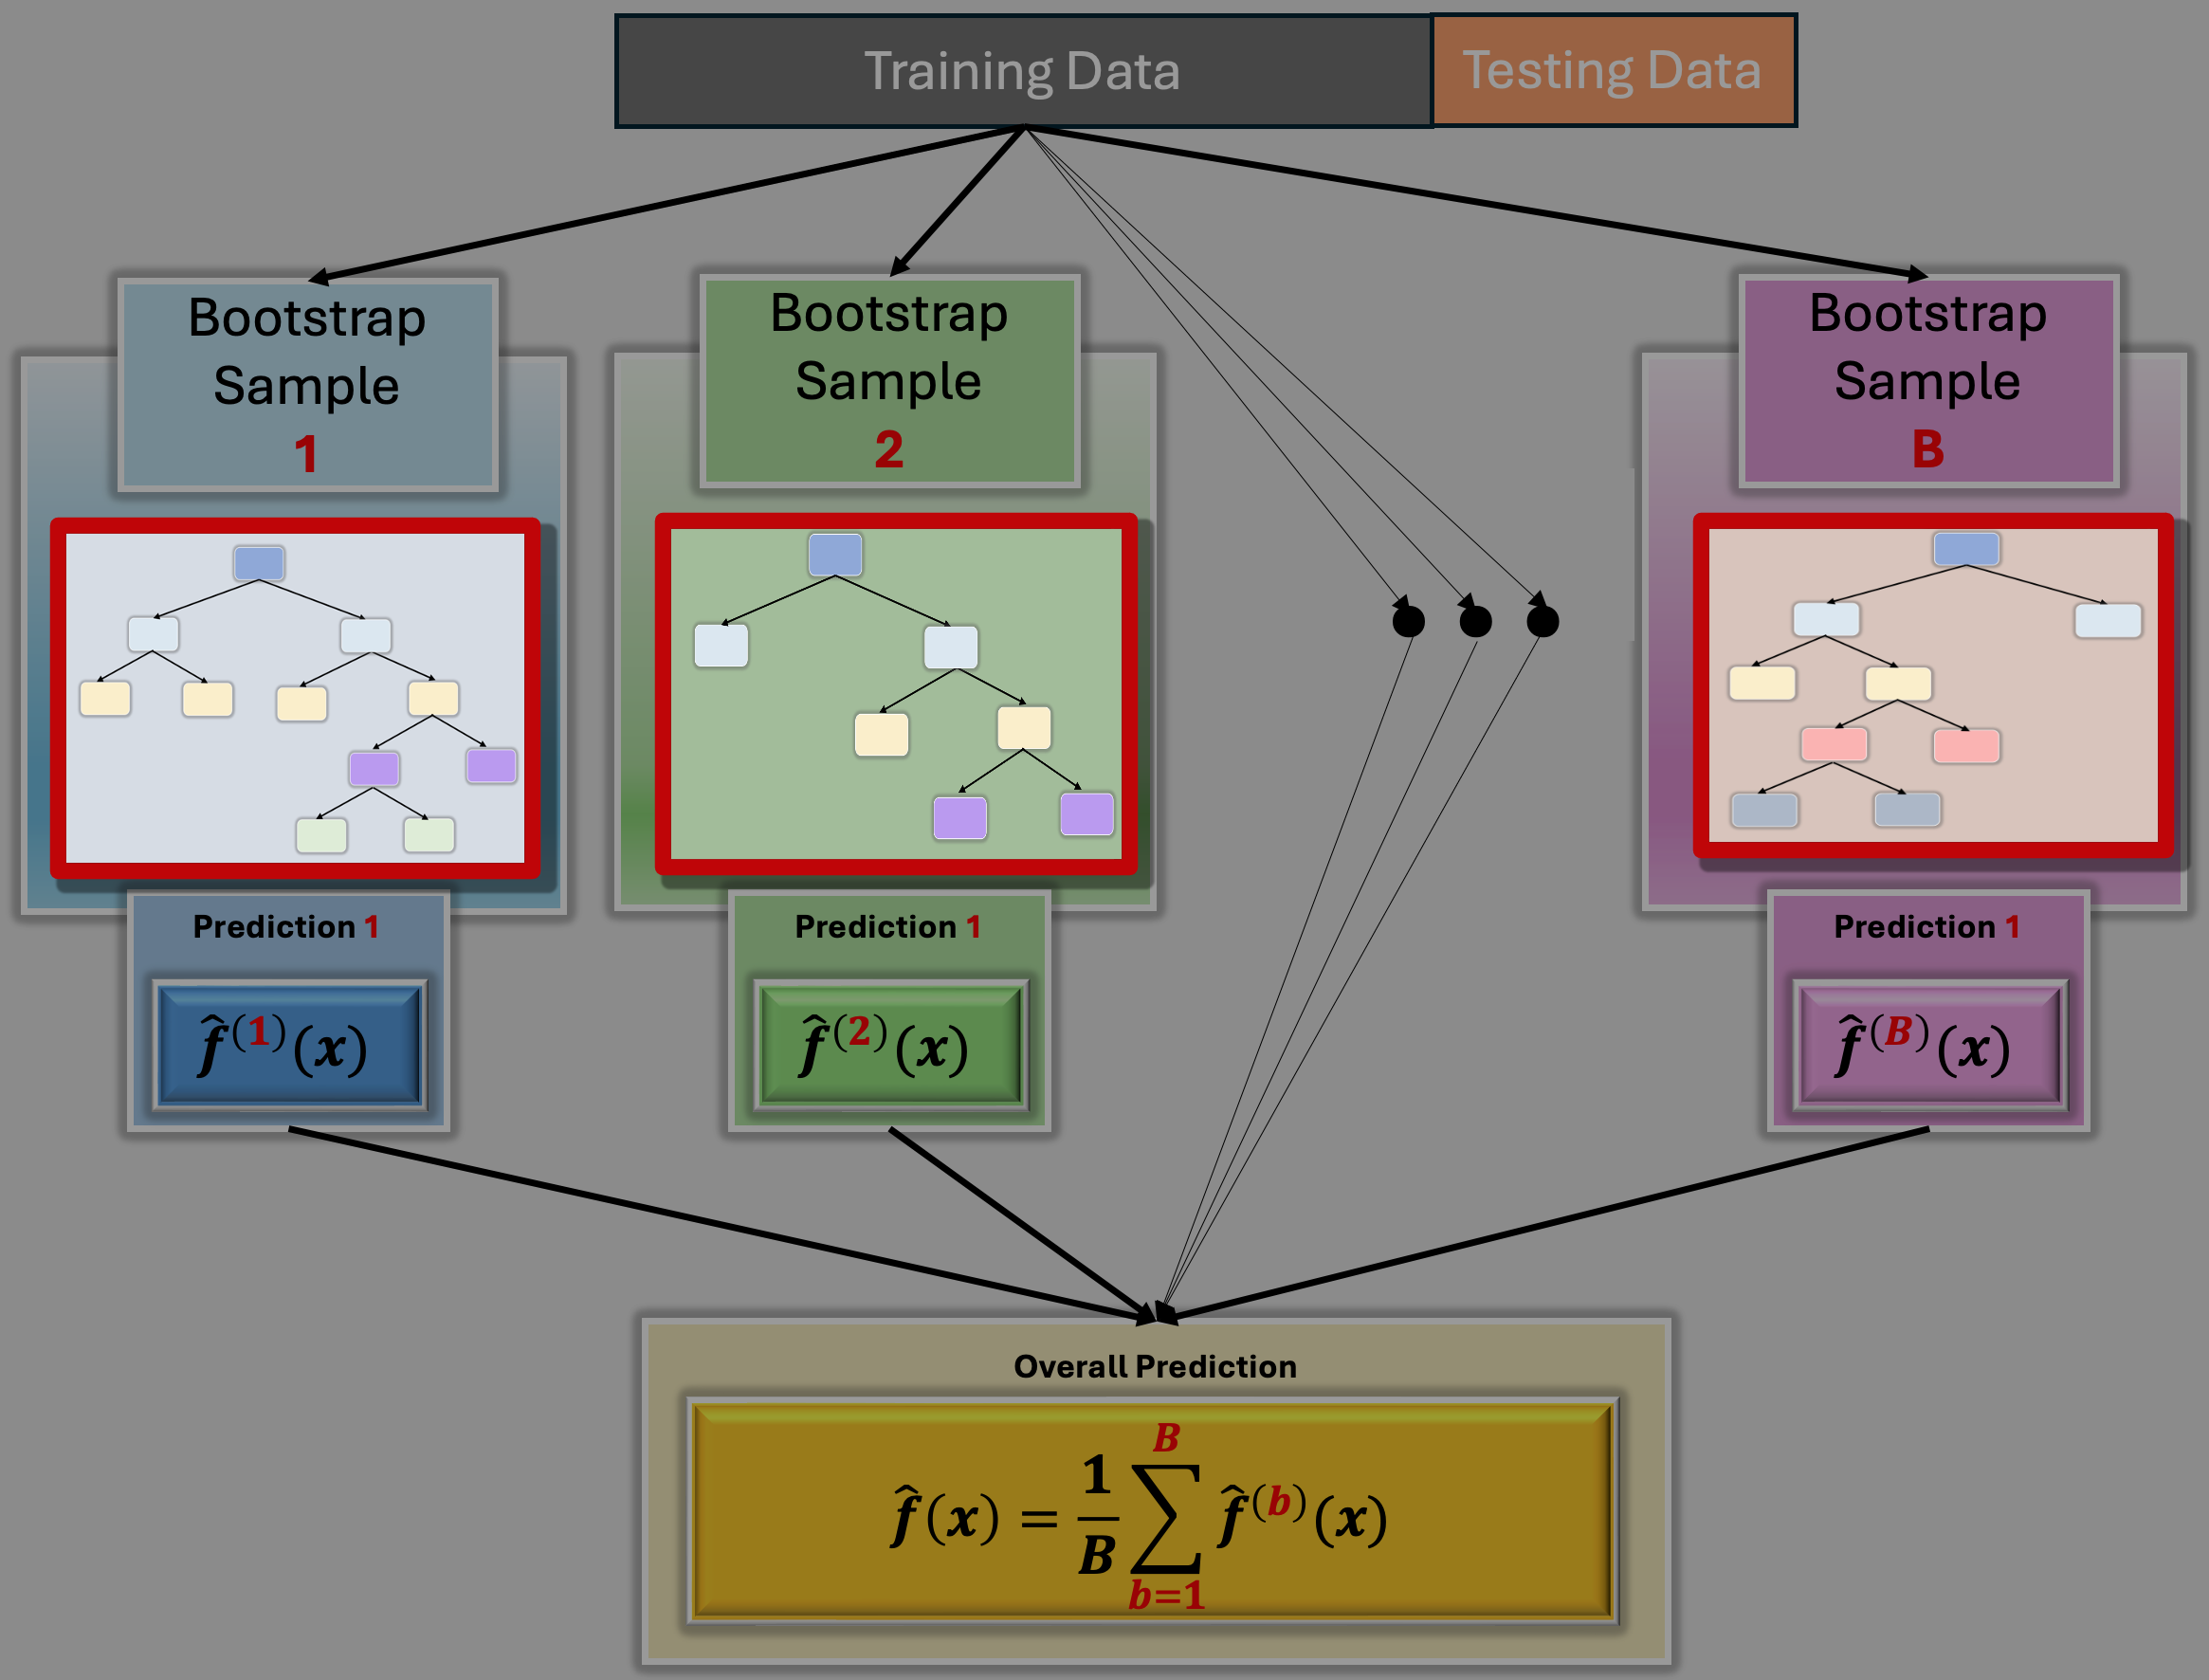
\includegraphics[scale=.25]{fig/Random_Forest_Tree.png}
\end{center}
}\\
\end{frame}




{
 \setbeamercolor{background canvas}{bg=}
%
\includepdf[pages={1}, scale=1, trim=1mm 5mm 11mm 5mm]{STAT380-Unit2.pdf}
\includepdf[pages={16-18}, scale=1]{STAT380-Unit4.pdf}
}




\section{Boosting}
\TransitionFrame[airforceblue]{\Large Boosting }

{\setbeamercolor{background canvas}{bg=}
\includepdf[pages={20-22}, scale=1]{STAT380-Unit4.pdf}
}



\begin{frame}\frametitle{Adaptive Boosting (Binary Classification): Idea}
\qBrd[4.5in]{slateblue!50}{
\begin{center}
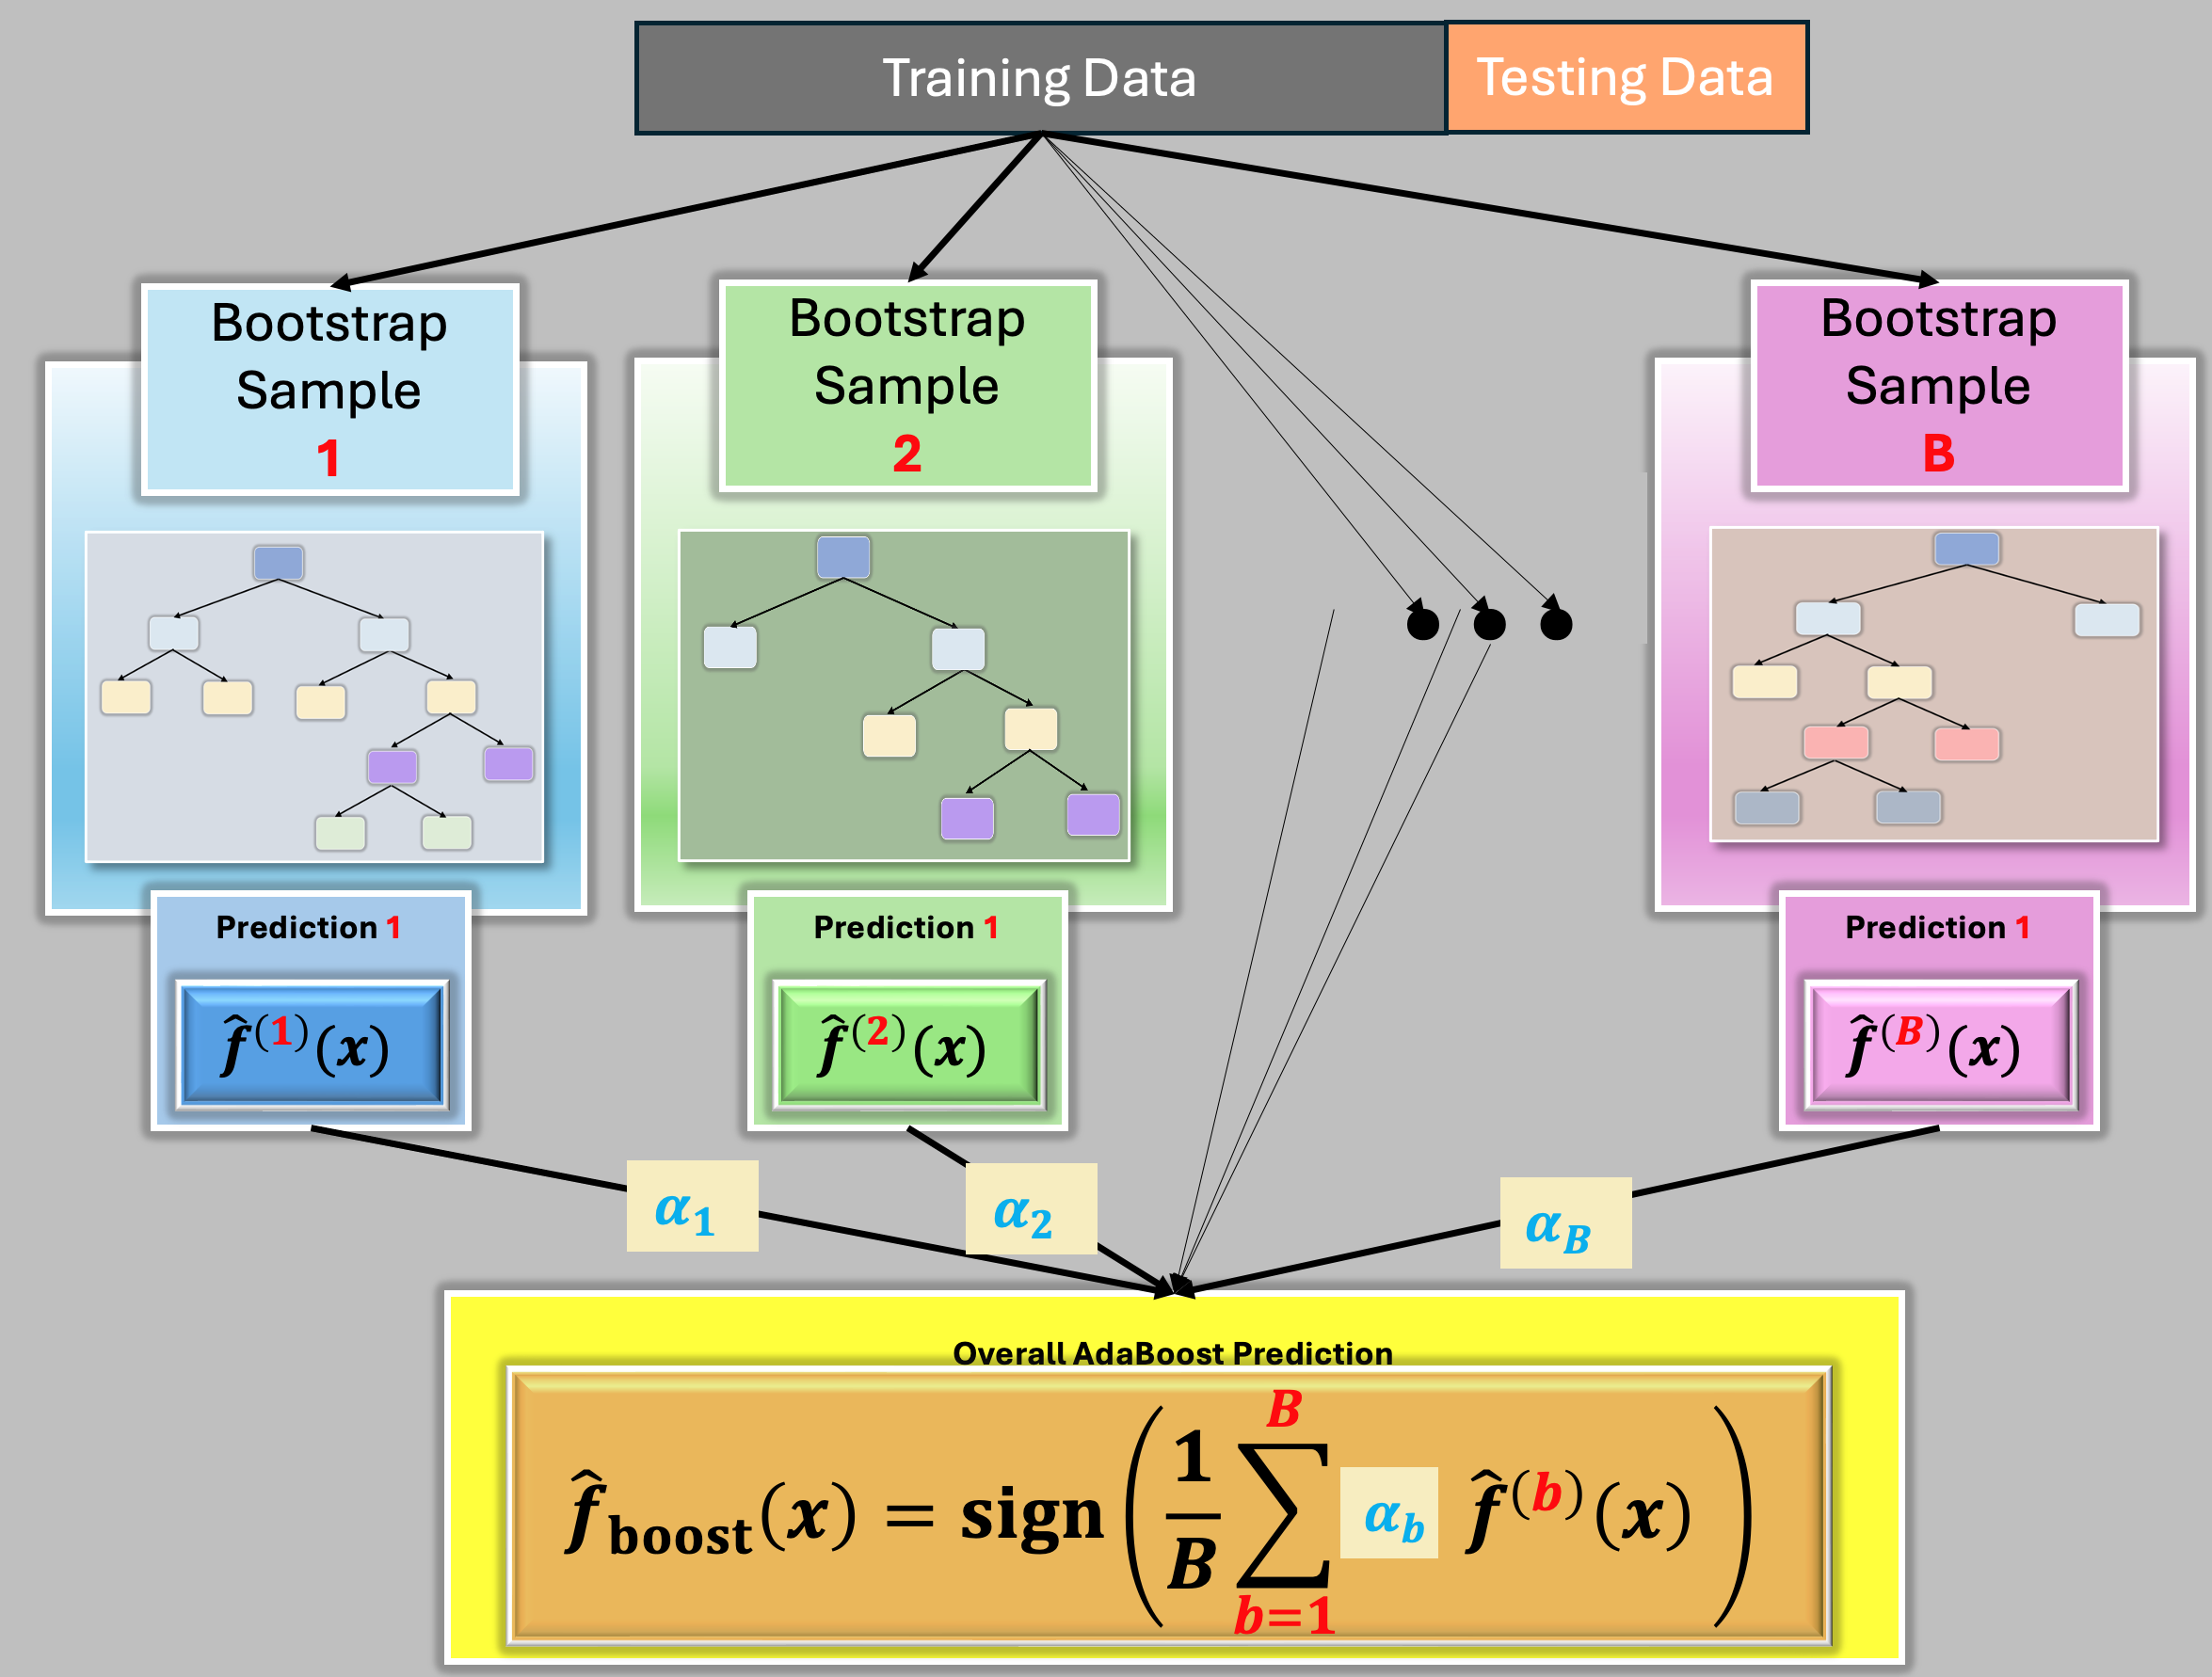
\includegraphics[scale=.24]{fig/AdaBoost_Diagram_1.png}
\end{center}
}\\
\end{frame}

\begin{frame}\frametitle{Adaptive Boosting (Binary Classification) Algorithm}
\qBrd[4.5in]{slateblue!50}{
\begin{center}
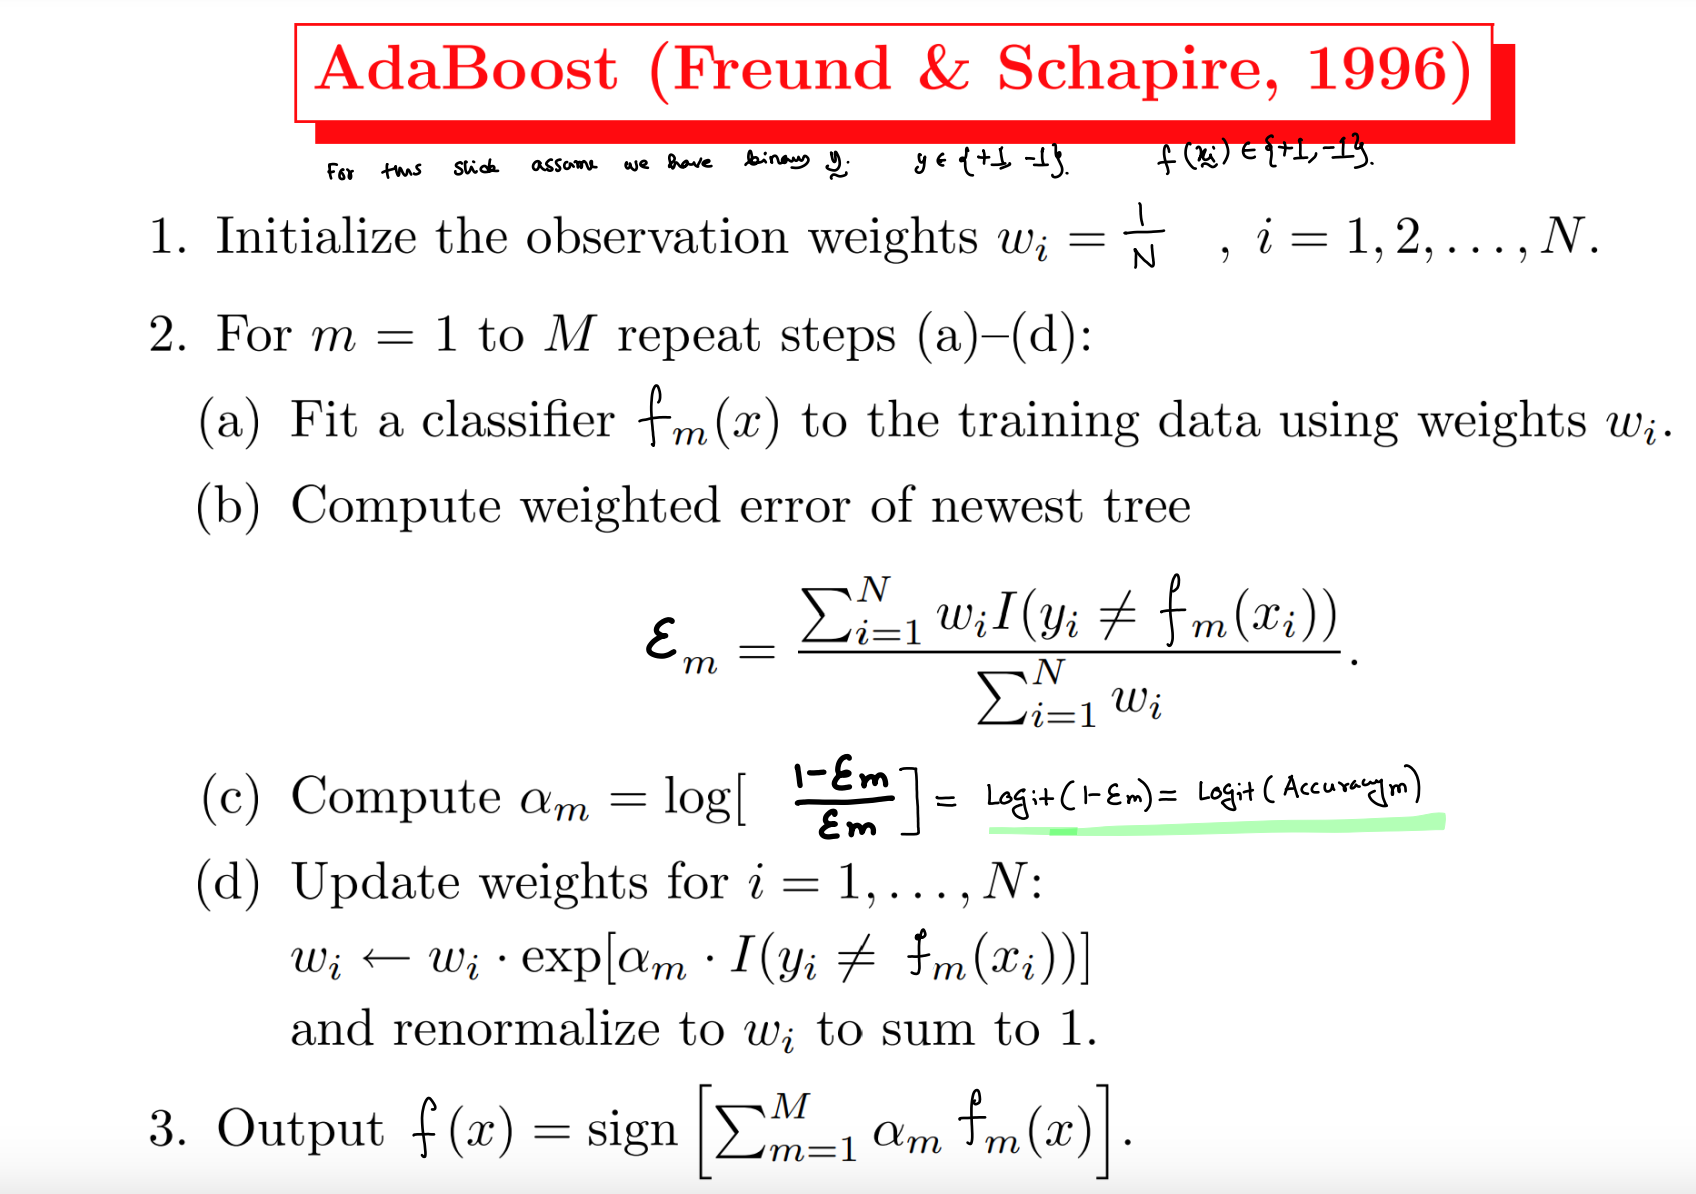
\includegraphics[scale=.35]{fig/AdaBoostAlgo1.png}
\end{center}
}\\
\end{frame}


\begin{frame}\frametitle{Adaptive Boosting (Binary Classification) Algorithm}
\qBrd[4.5in]{apricot!50}{
\begin{center}
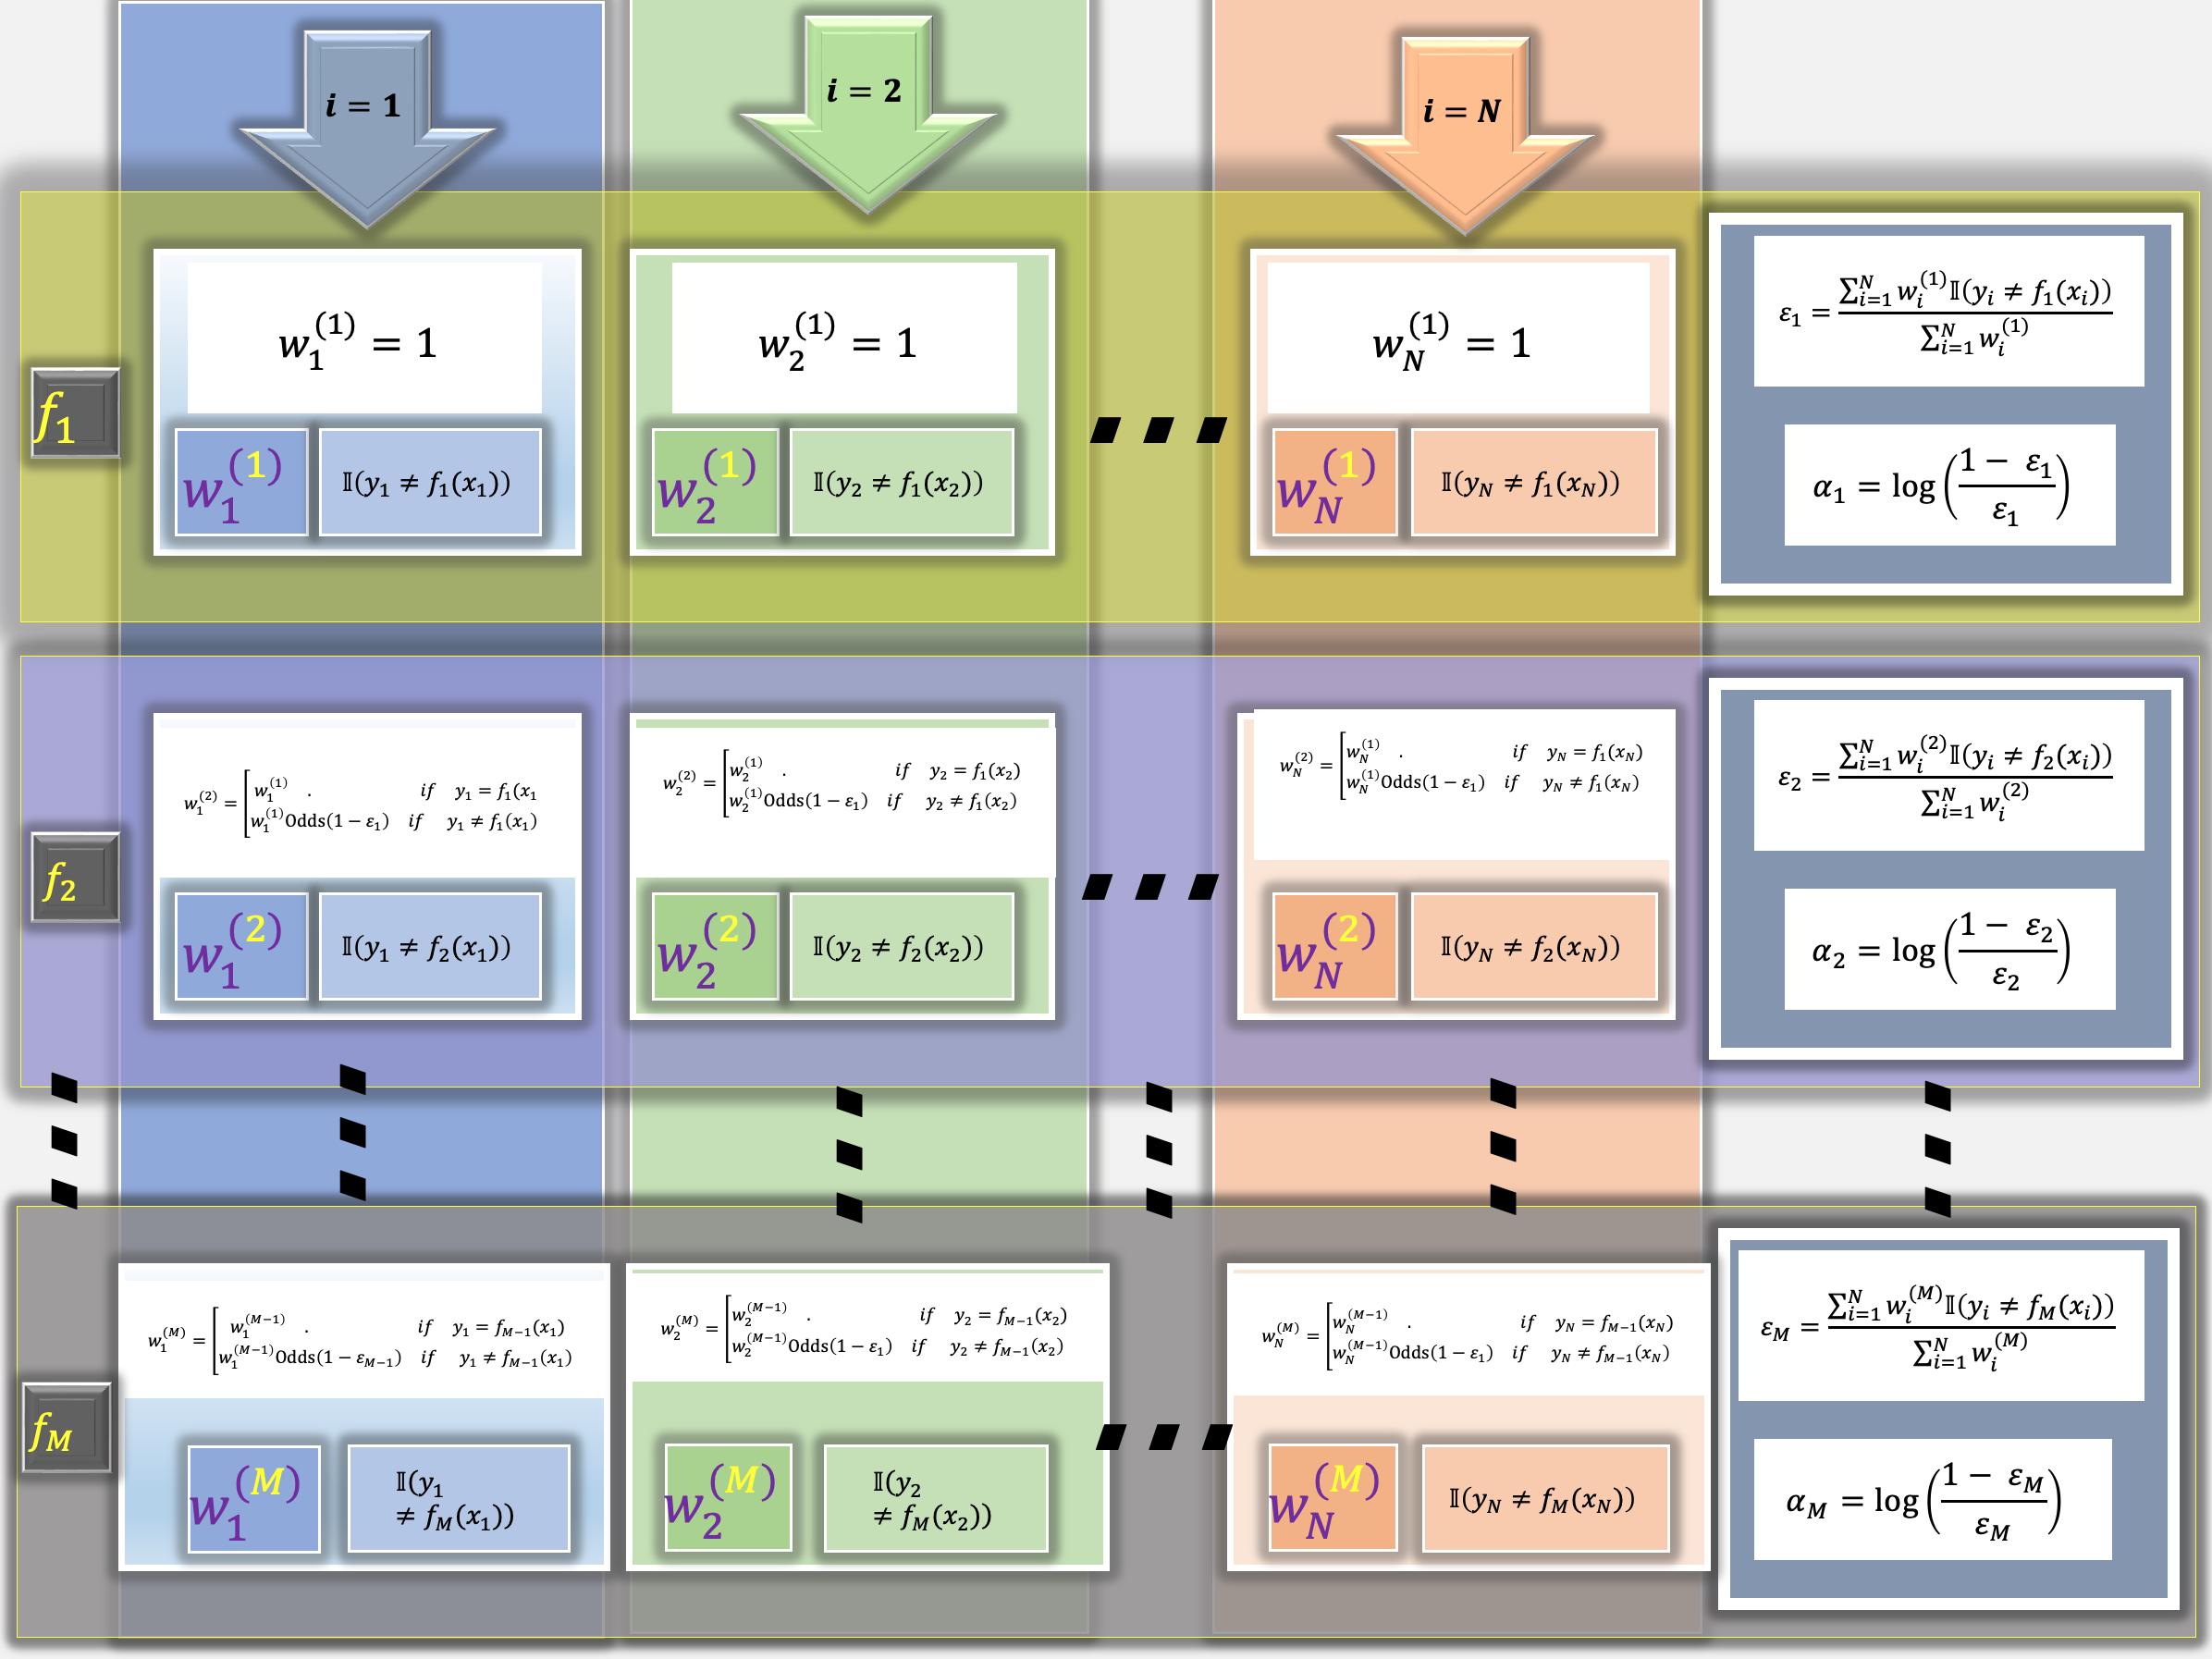
\includegraphics[scale=.24]{fig/AdaBoostTable1.png}
\end{center}
}\\
\end{frame}


\begin{frame}\frametitle{Adaptive Boosting (Binary Classification) Algorithm}
\qBrd[4.5in]{slateblue!50}{
\begin{center}
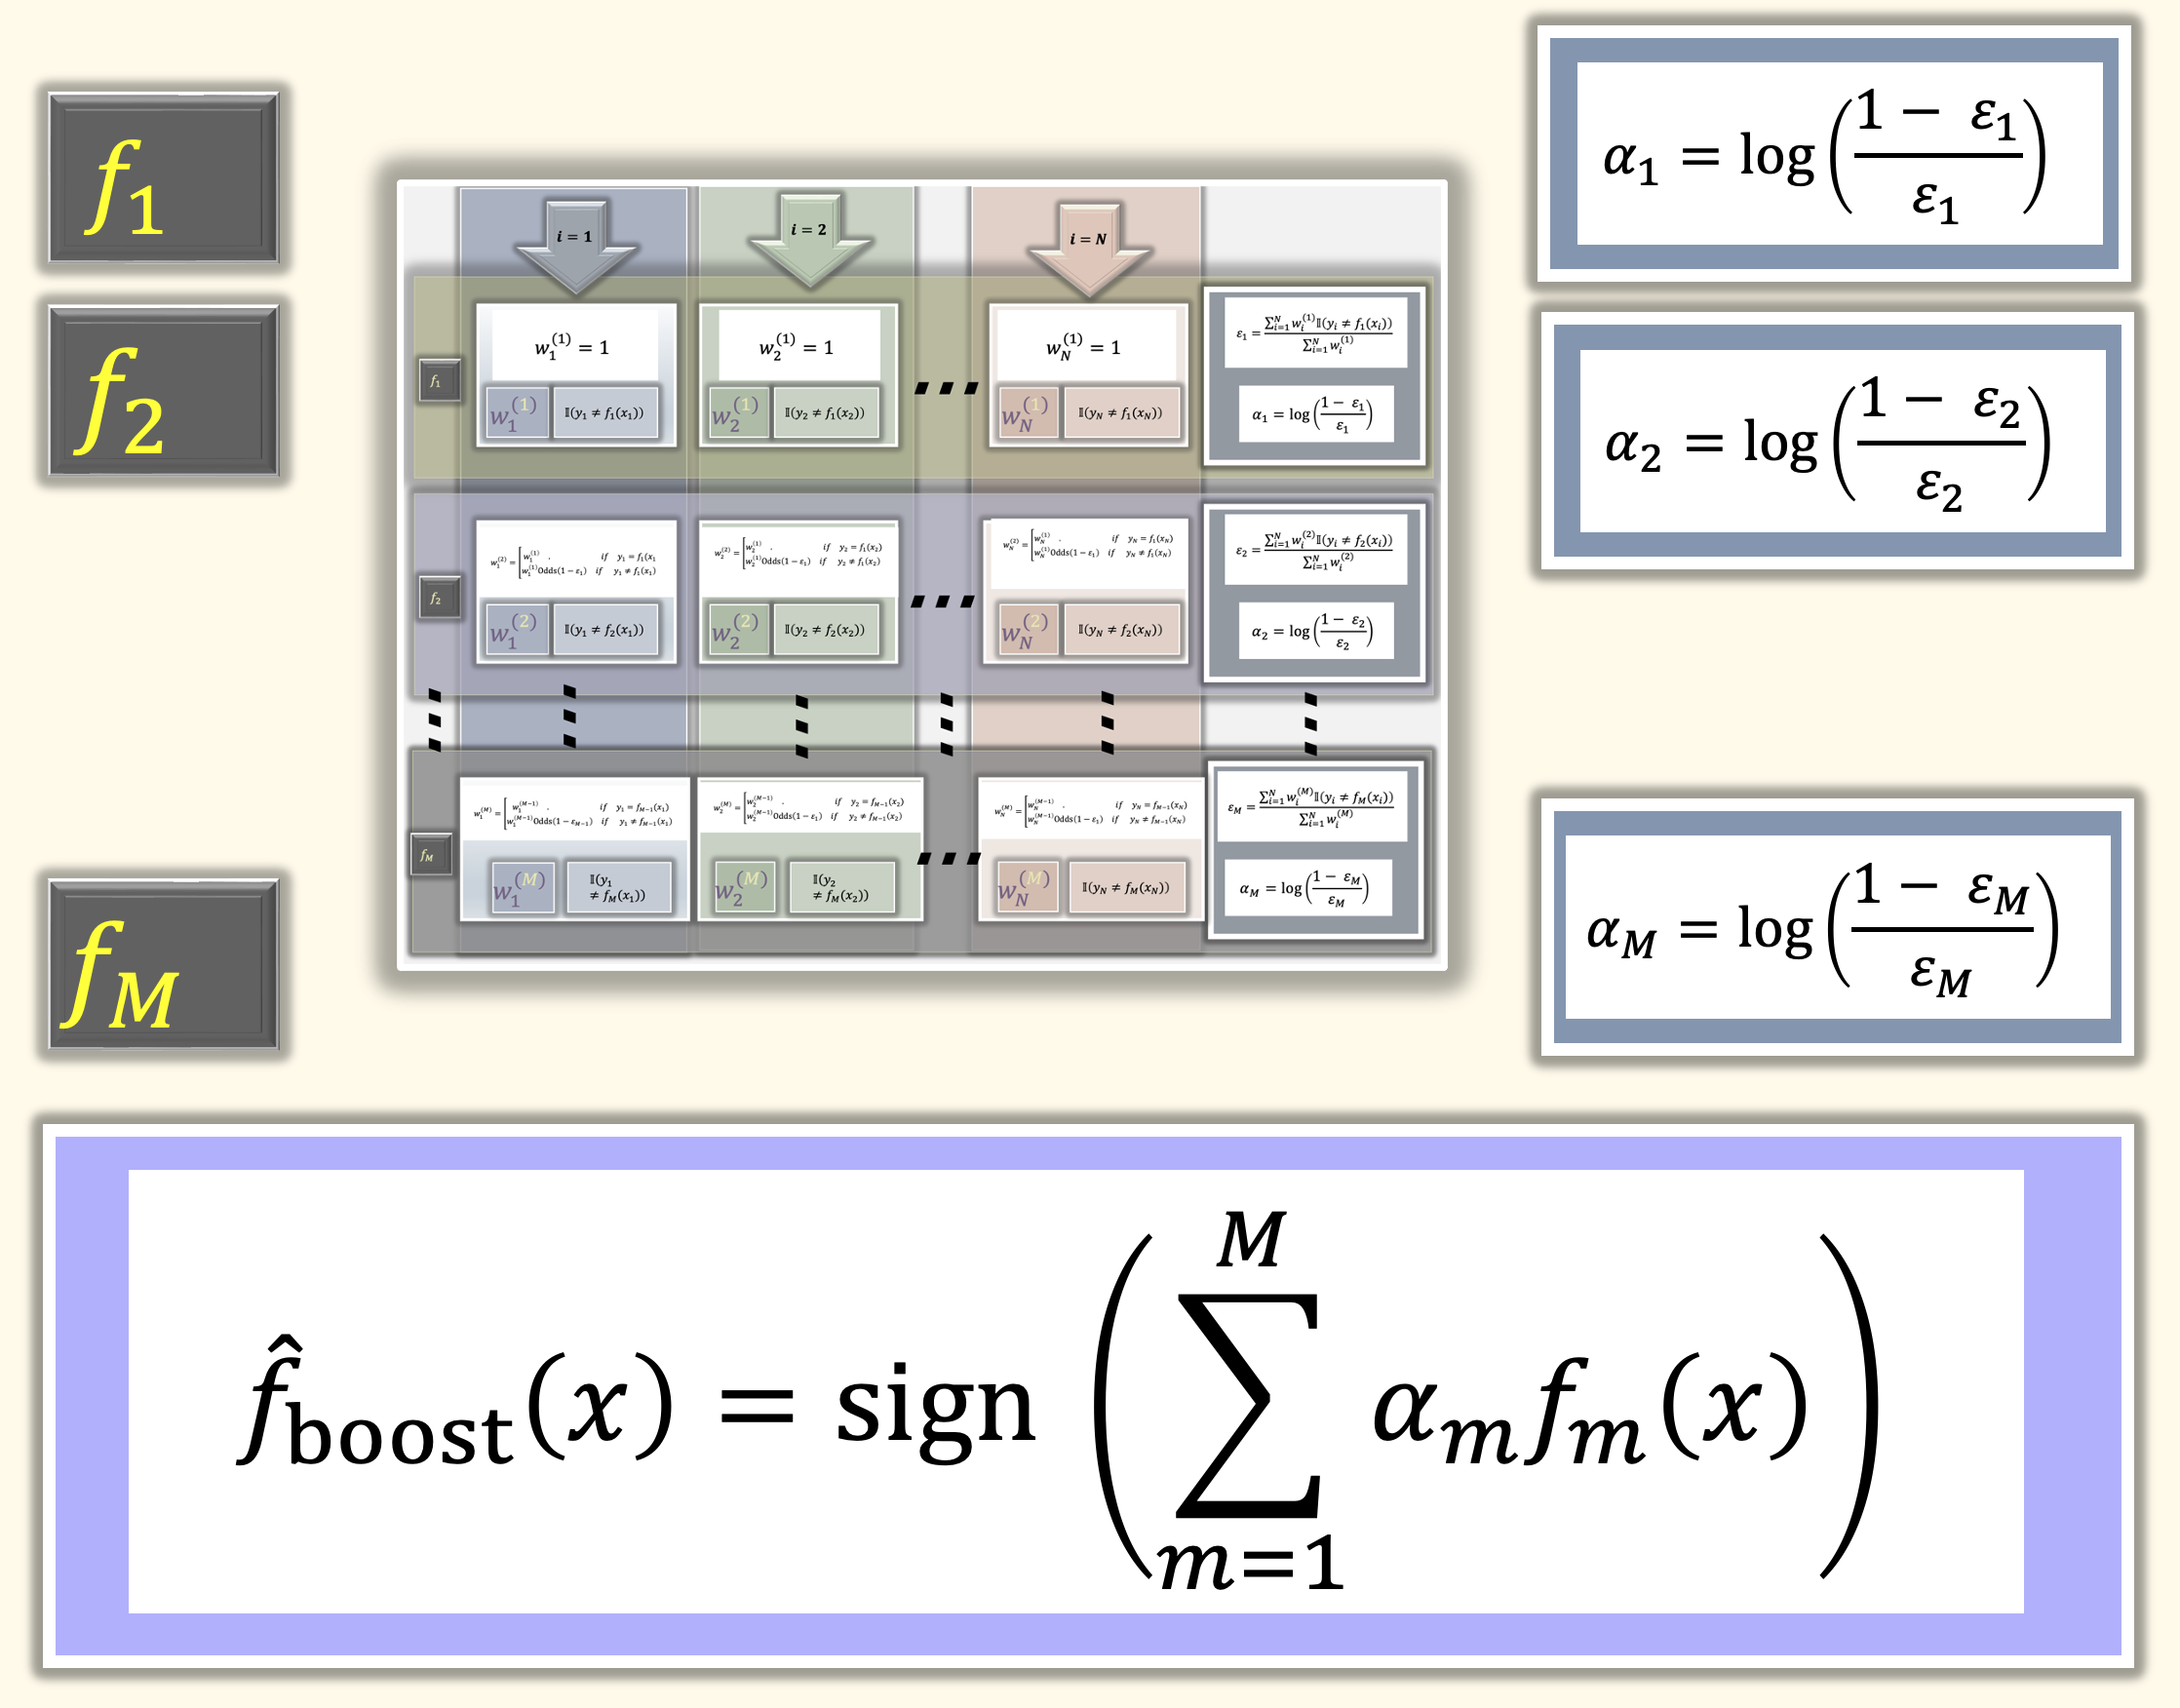
\includegraphics[scale=.22]{fig/AdaBoostTable2.png}
\end{center}
}\\
\end{frame}



\begin{frame}\frametitle{AdaBoost: A Toy Example}
\qBrd[4.5in]{slateblue!50}{
\begin{center}
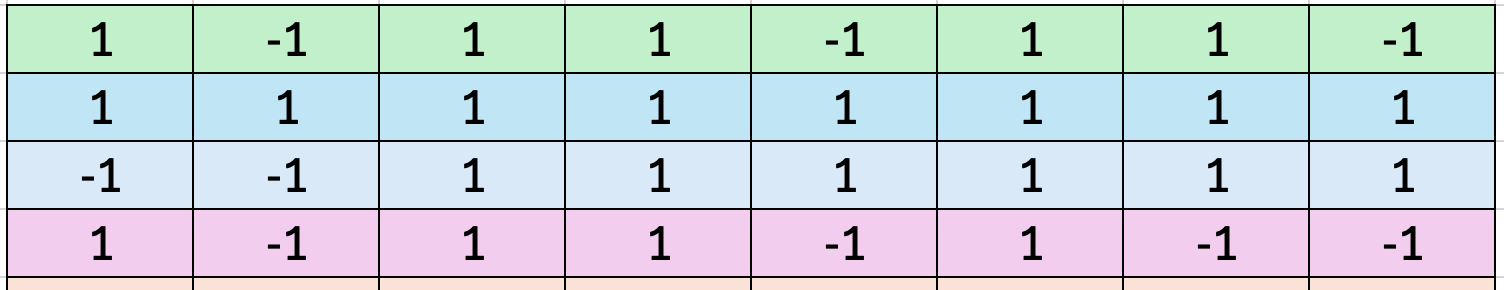
\includegraphics[scale=.35]{fig/AdaBoost_toyData.png}
\end{center}
}\\
\vspace{1in}
\end{frame}

\begin{frame}
%\qBrd[4.5in]{slateblue!50}{
\vspace{-.5in}
\begin{center}
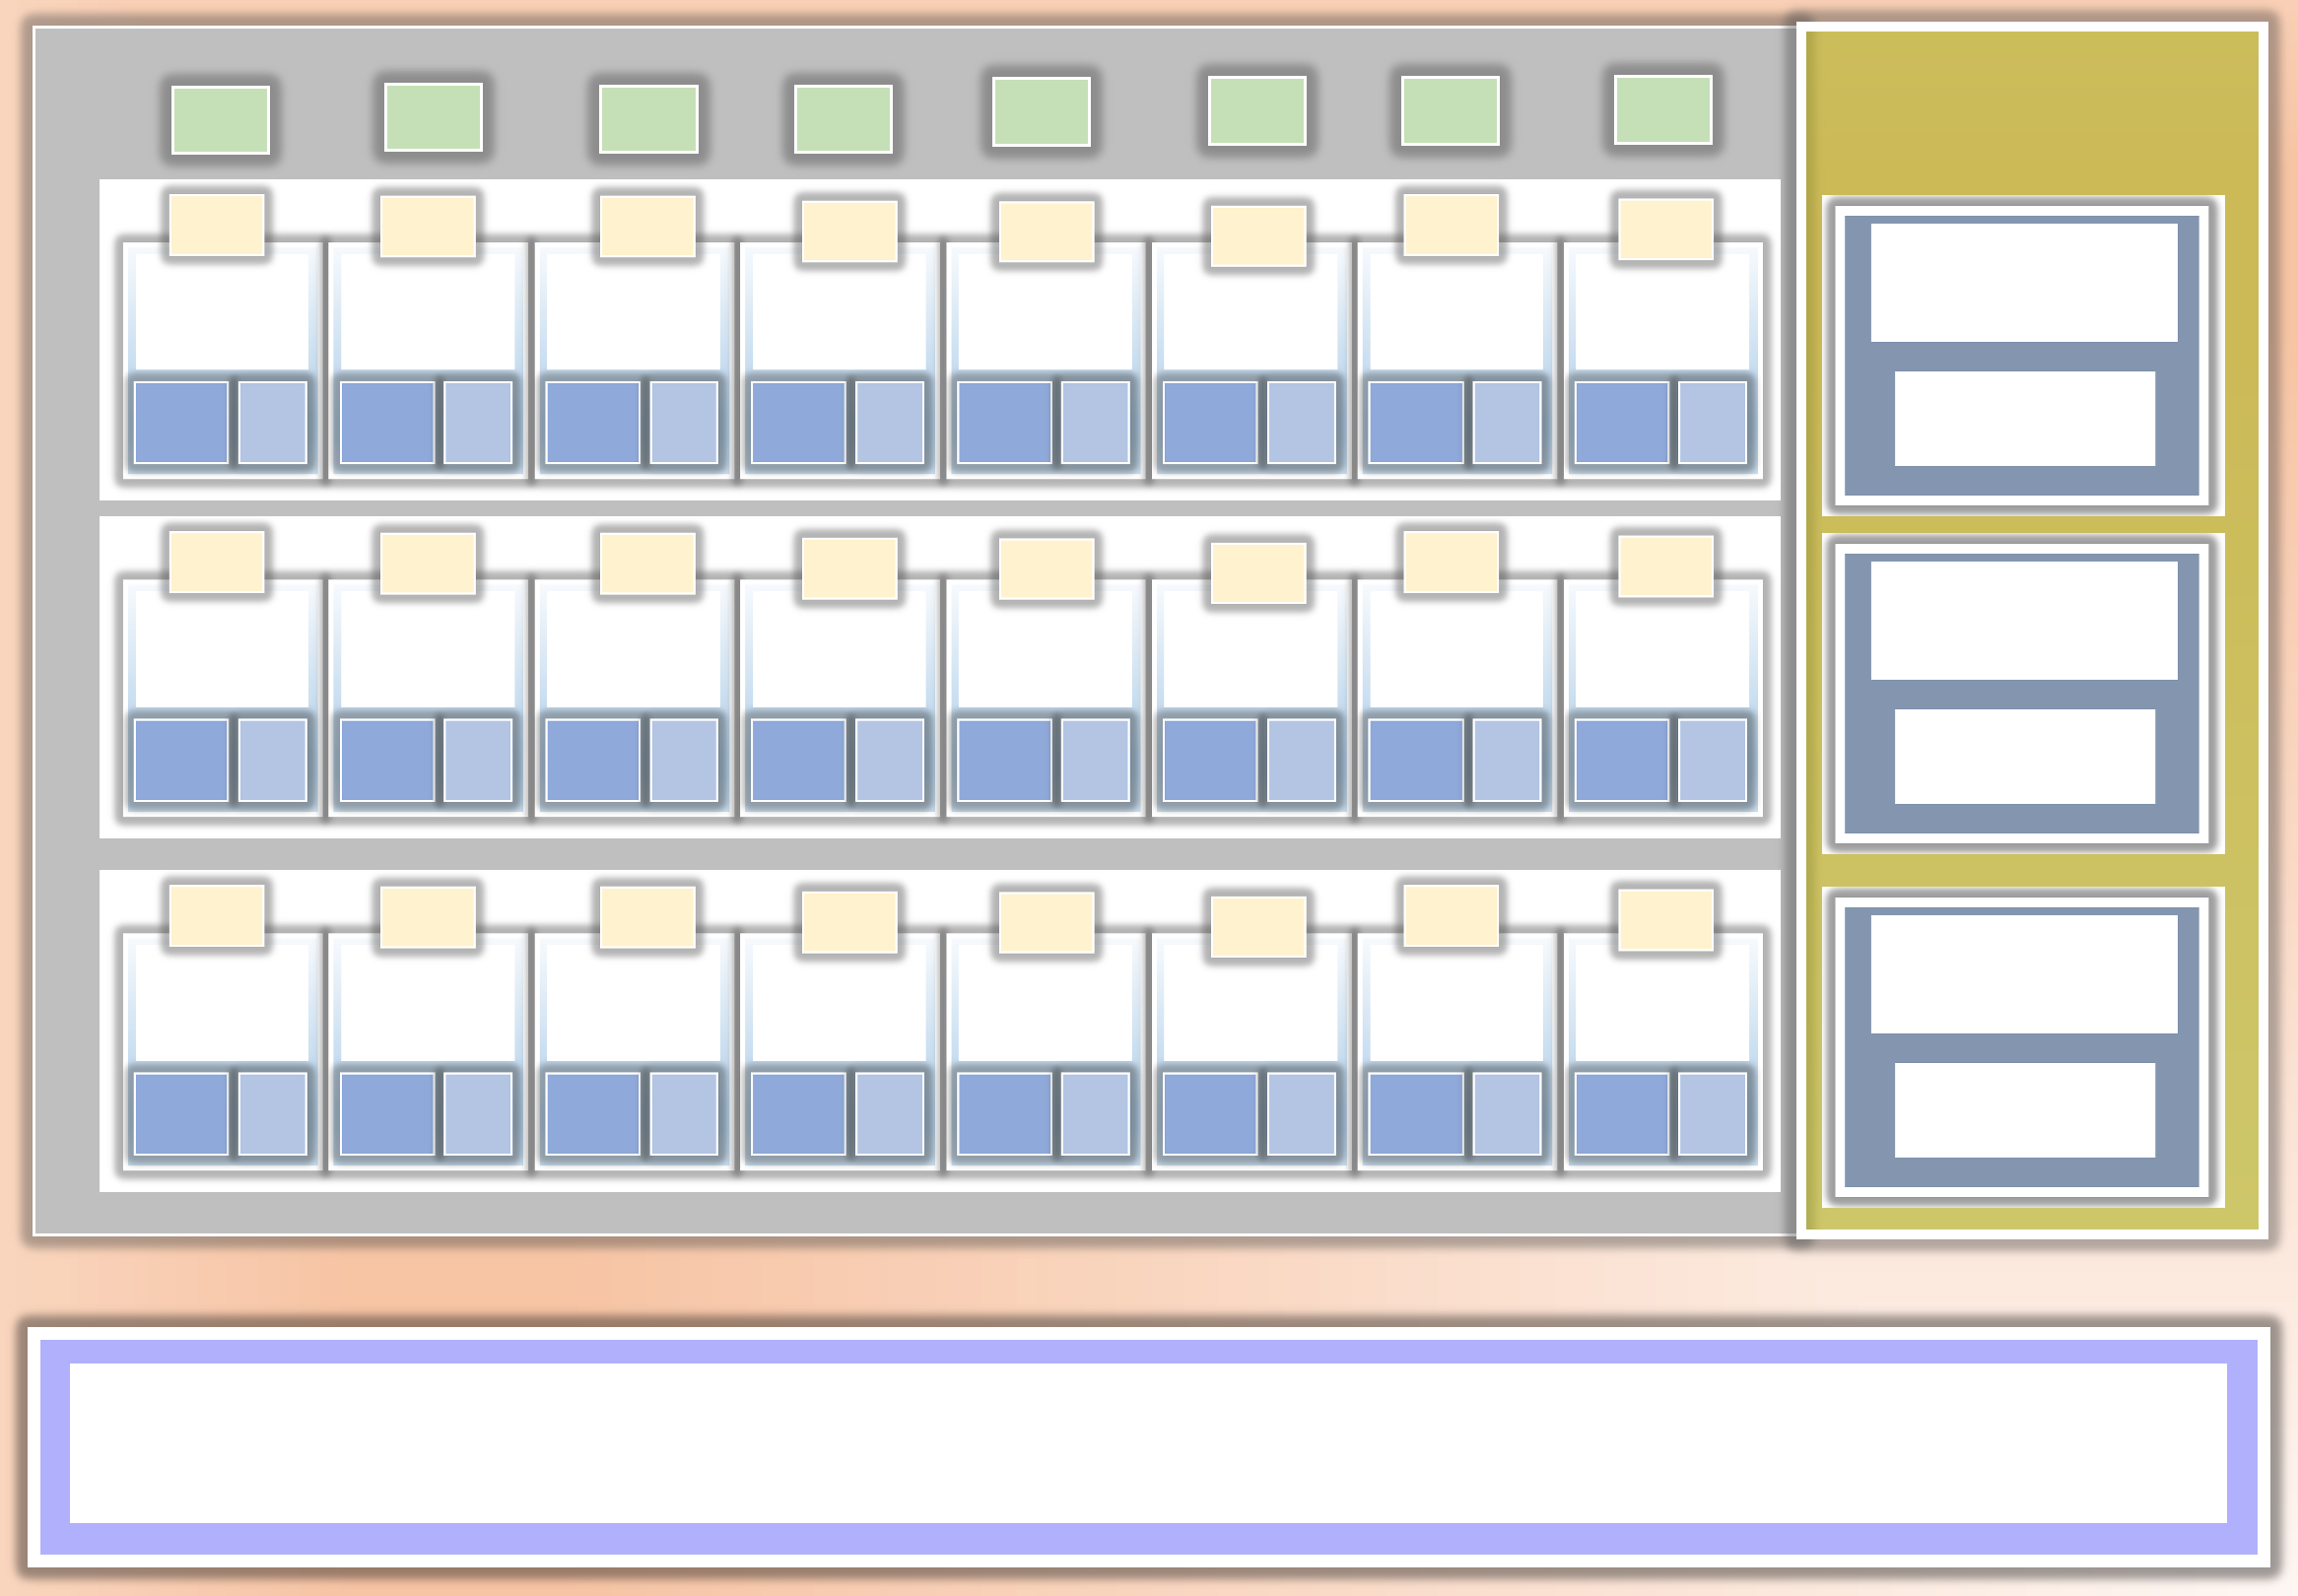
\includegraphics[scale=.3]{fig/AdaBoost_Toy_Example.png}
\end{center}
%}\\
\end{frame}

{\setbeamercolor{background canvas}{bg=}
\includepdf[pages={27}, scale=1]{STAT380-Unit4.pdf}
}




%
%\begin{frame}
%\DefBoxOne{Regression Tree: Fitted Equation }{\color{black}
%Let $(y_i, \bx_i)\in \R\times \R^{p}$ for $i=1, \ldots n $ are observed data.  The mathemetical representation of the fitted equation of a Regression Tree is $\HLTW{\hat{y} = f(\bx)}$, where \\
%\qBrd[4.1in]{babyblueeyes!40}{ $$\HLTW{ \displaystyle f(\bx )= \sum_{j=1}^{J} \HLTEQ[purple!40]{\HLTY{c_j }}\; \HLTEQ[babyblue!40]{ \Indicator{\bx \in \HLTEQ[rose!40]{\HLTY{R_j}}}} } $$}
%}\\
%%\vspace{.1in}
%%\qBrd[4.5in]{teal!40}{  
%%\begin{center}
%%\HLTEQ{\bRdg= (\bX^T\bX+\lambda I_p)^{-1}\bX^T{\bf y},}
%%\end{center}
%%}
%\end{frame}
%
%
%
%
%
%
%
%
%\begin{frame}
%\qBrd[4.1in]{babyblueeyes!50}{ $$\HLTW{ \displaystyle f(\bx )= \sum_{j=1}^{J} \HLTEQ[purple!40]{\HLTY{c_j }}\; \HLTEQ[babyblue!40]{ \Indicator{\bx \in \HLTEQ[rose!40]{\HLTY{R_j}}}} } $$}\\
%\qBrd[4.1in]{babyblueeyes!60}{ $$\HLTW{ \displaystyle
%\text{SSE}:= \sum_{i=1}^n \left(y_i -f(\bx_i) \right)^2
% } =   \DBX{\HLTW{ \displaystyle \sum_{j=1}^J  \sum_{i\in \HLTEQ[rose!40]{\HLTY{ R_j}}}^{}\left(y_i - \HLTY{ \widehat{c}_j} \right)^2  }}$$}\\
% 
%$$\DBX{ \HLTY{ \displaystyle  \widehat{c}_j}  =  \frac{1}{n_j} \sum_{i \in R_j } y_i    }$$
%\end{frame}
%
%
%
%\begin{frame}
%\qBrd[4.5in]{babyblueeyes!50}{
%\begin{center}
%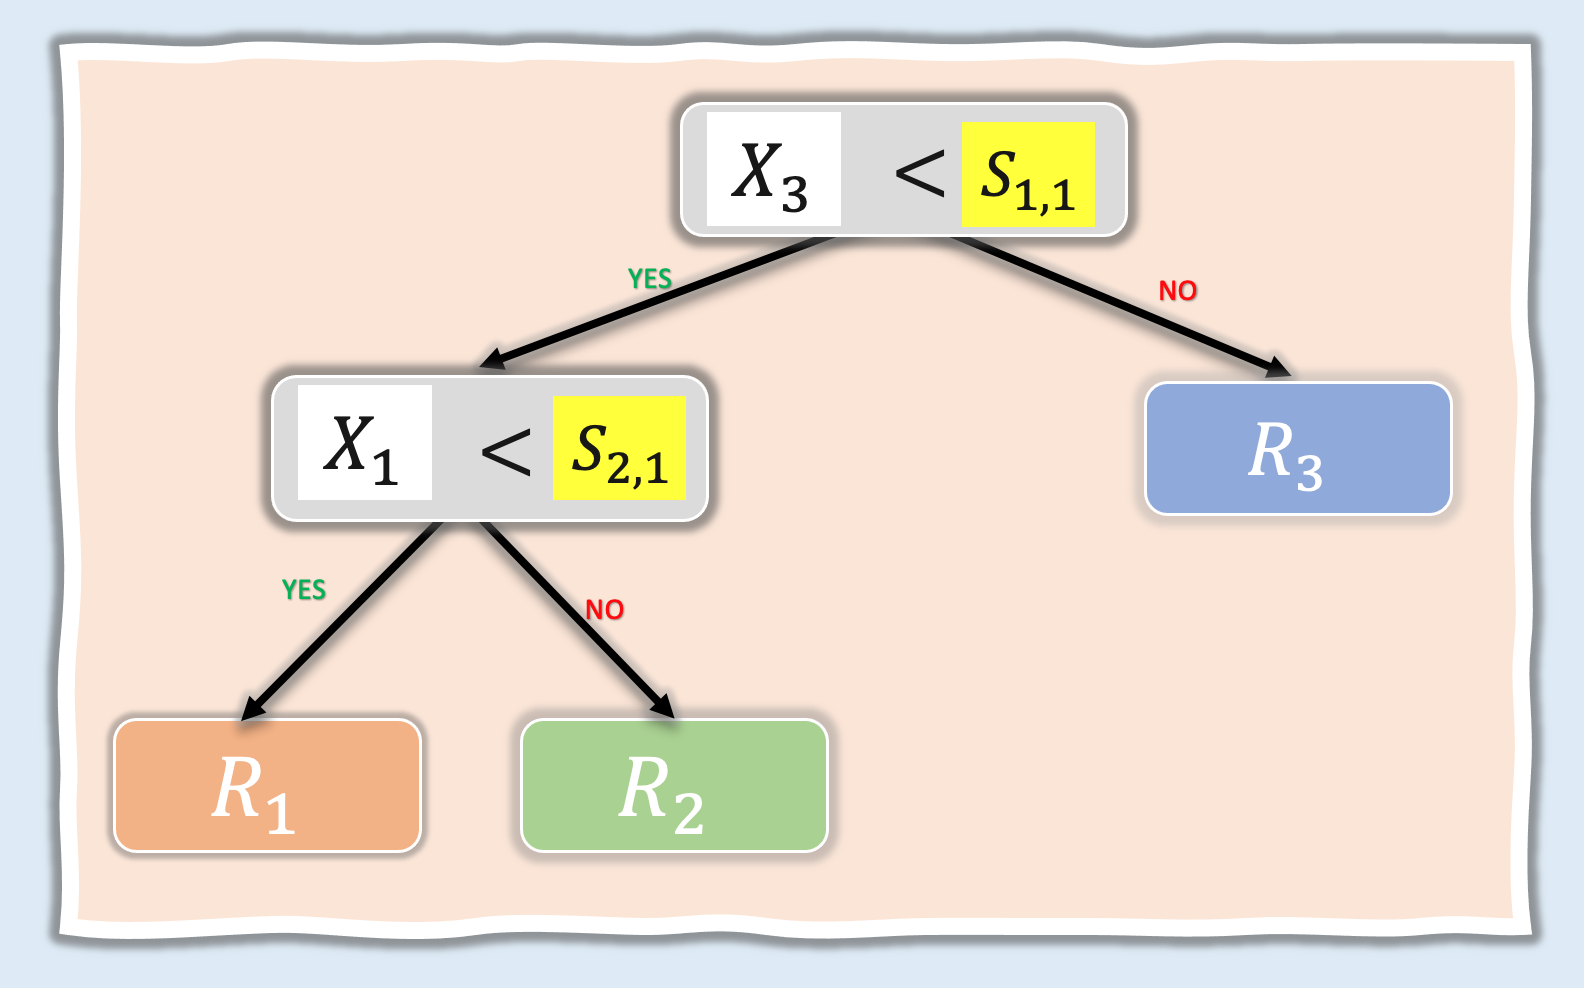
\includegraphics[scale=.32]{figs/RegressionTreeDiagram.png}
%\end{center}
%%\vspace{.1in}
%\begin{enumerate}
%\qBrd[4in]{airforceblue!50}{
%\item[\sqBullet{bluebell}] How do we decide which varibale to select while creating the binary split? i.e. which one among  $\HLTW{\{X_1, \ldots X_p\}}$
%}
%\qBrd[4in]{babyblue!50}{
%\item[\sqBullet{babyblue}]  How do we select the cut off $\HLTY{S}$?
%}
%\end{enumerate}
%}\\
%\vspace{.2in}
%
%\end{frame}
%
%
%
%
%
%
%\begin{frame}
%\vspace{-.2in}
%\qBrd[4.5in]{babyblueeyes!50}{
%\begin{center}
%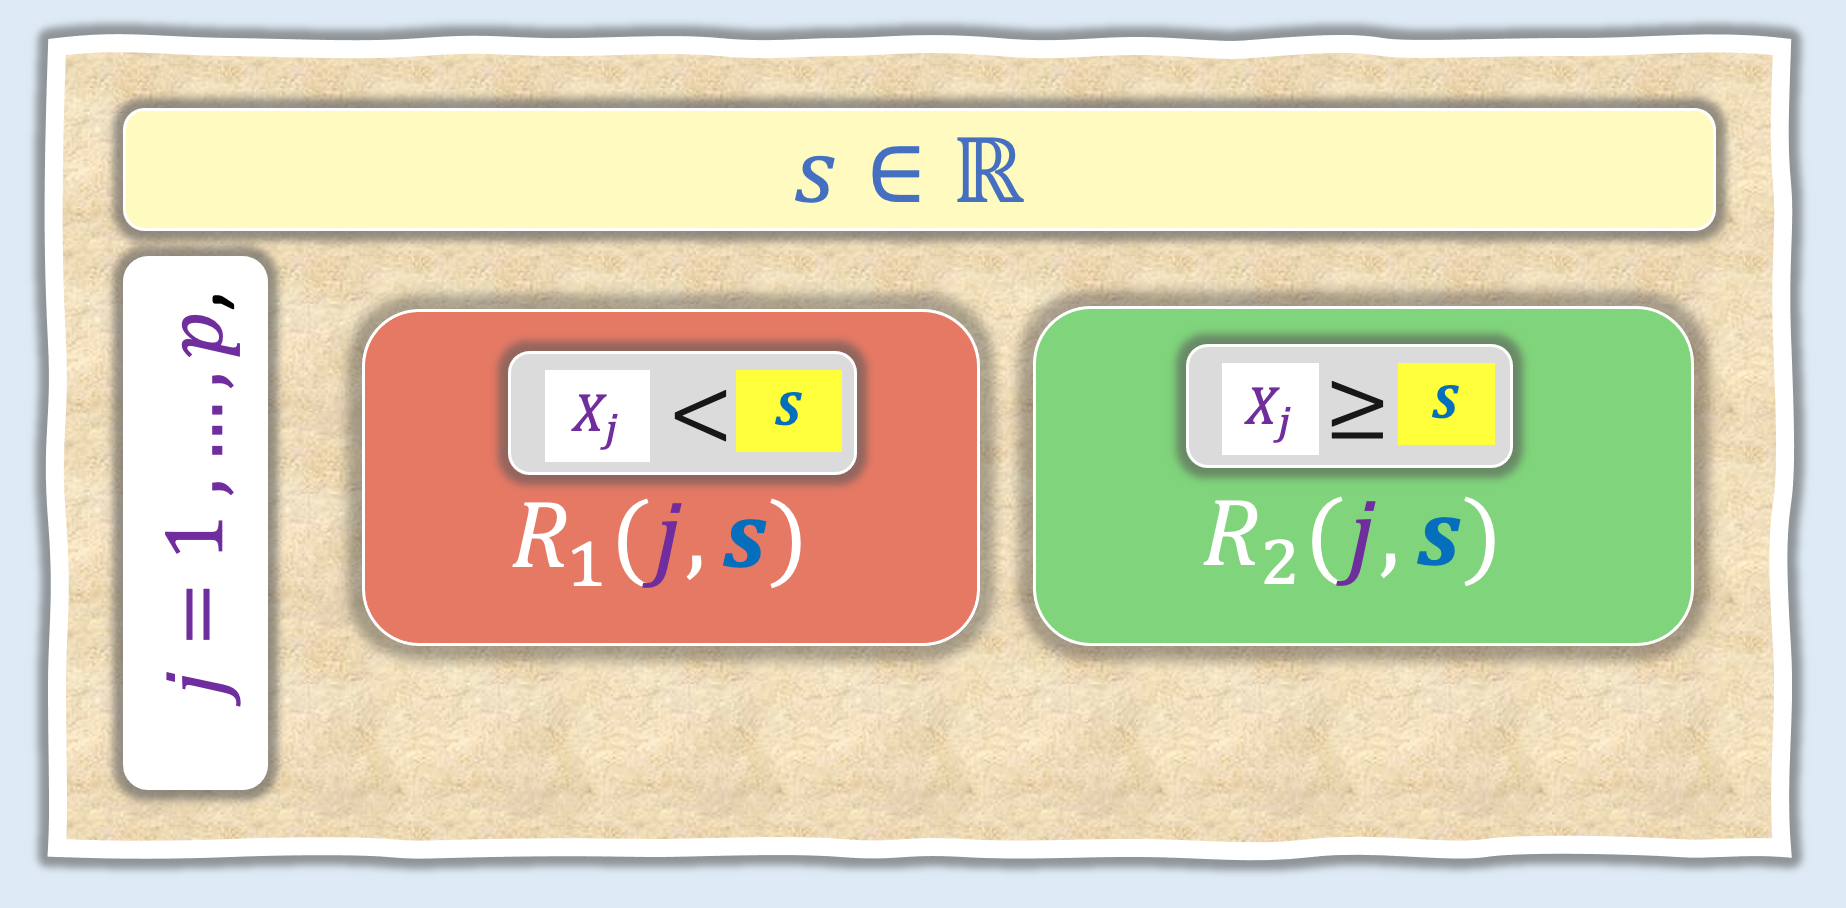
\includegraphics[scale=.3]{figs/R1_R2.png}
%\end{center}
%\vspace{-.15in}
%}\\
%\vspace{-.18in}
%\begin{center}
%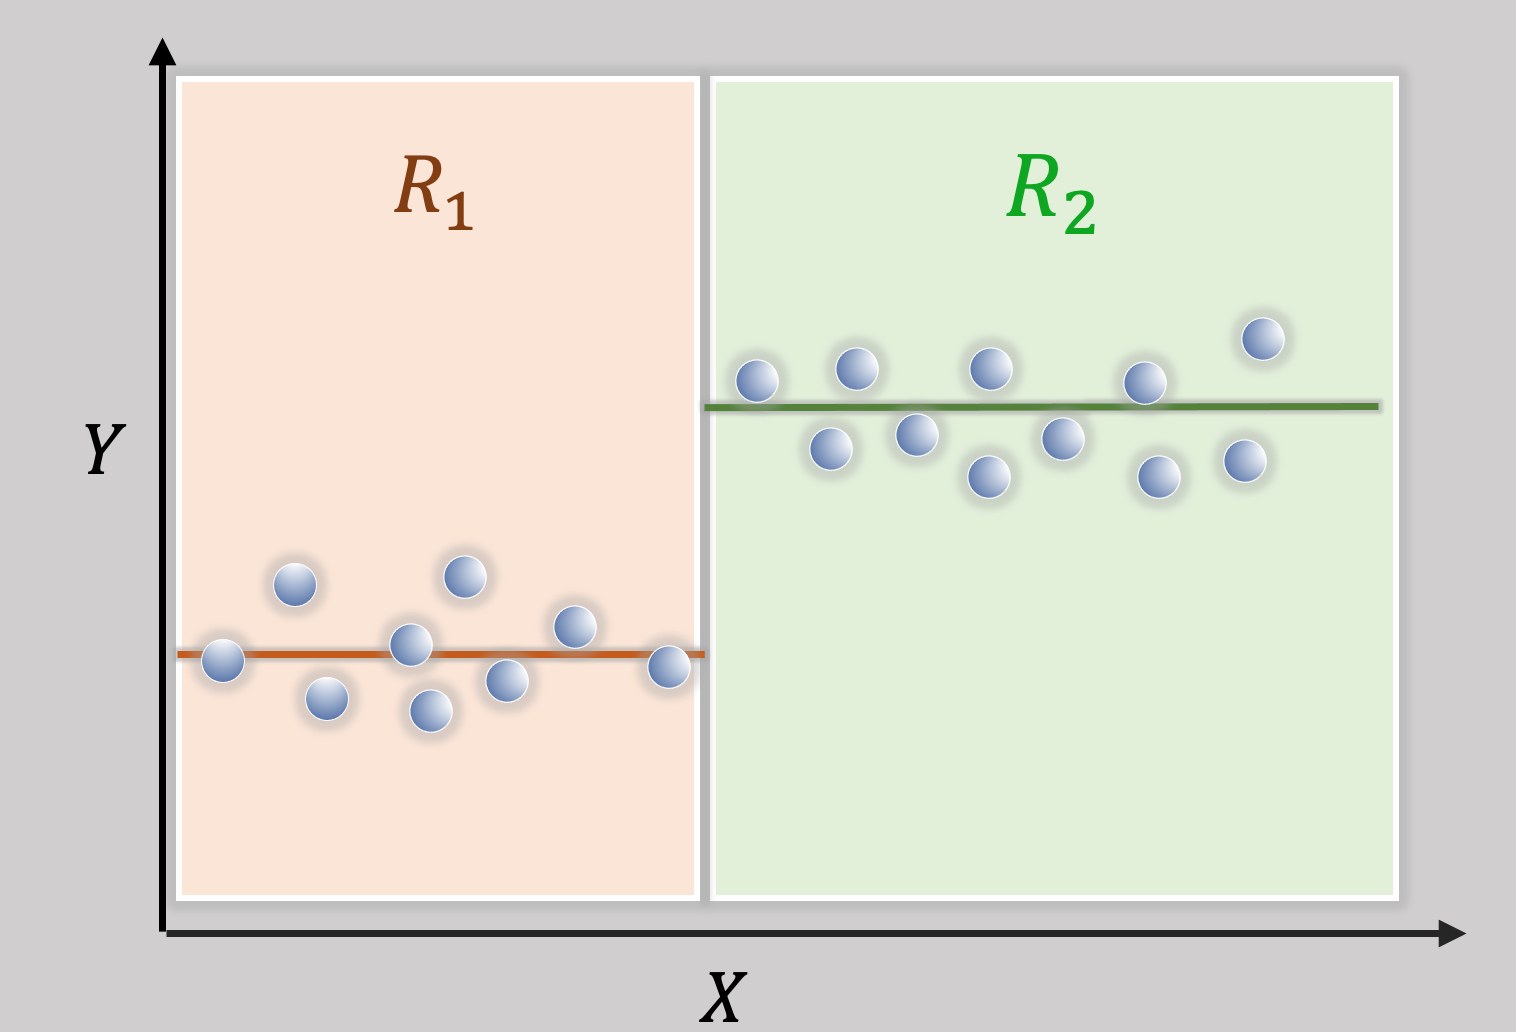
\includegraphics[scale=.22]{figs/RegressionTreeDiagram1.png}
%\end{center}
%\vspace{-.15in}
%\end{frame}
%
%
%
%\begin{frame}
%\qBrd[4.7in]{babyblueeyes!50}{
%\begin{center}
%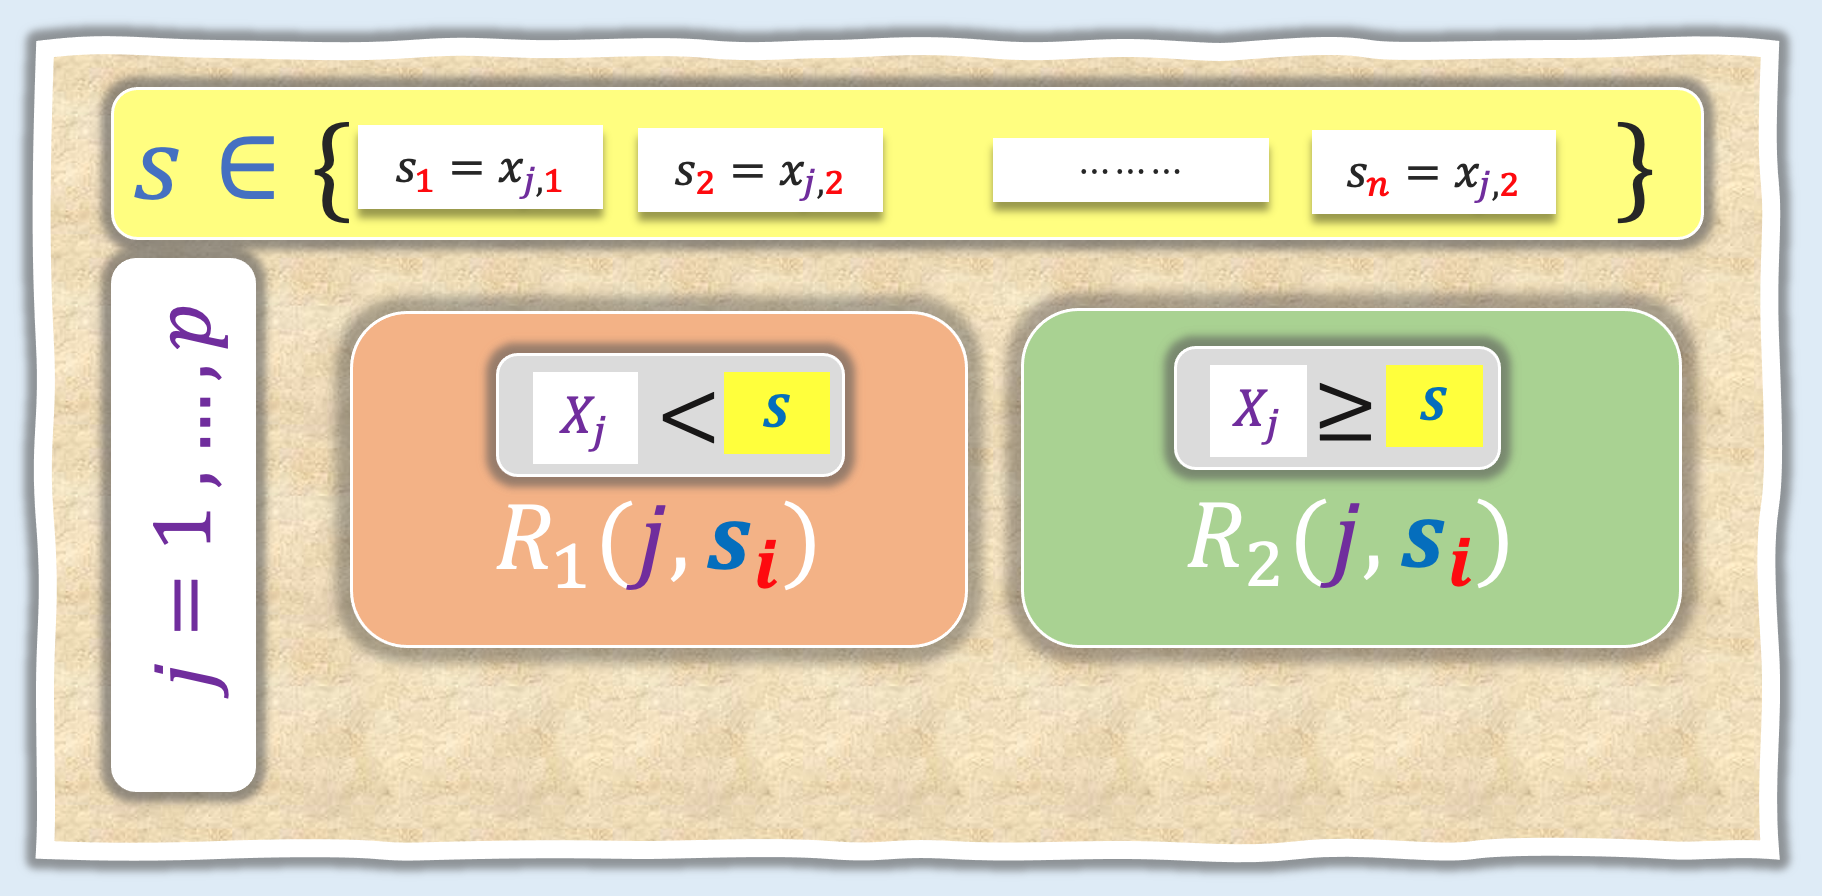
\includegraphics[scale=.35]{figs/R1_R2_s.png}
%\end{center}
%%\vspace{.1in}
%}\\
%\qBrd[4.7in]{airforceblue!50}{$$\HLTW{ \text{C}(j, s_i)}:=  {\HLTW{ \displaystyle  \sum_{\HLTEQ[rose!40]{i\in \HLTY{ R_1(j, s_i)}}}^{}\left(y_i - \HLTY{ \widehat{y}_{_{R_1}}} \right)^2  } + \HLTW{ \displaystyle  \sum_{ \HLTEQ[rose!40]{i\in \HLTY{ R_2(j, s_i)}}}^{}\left(y_i - \HLTY{ \widehat{y}_{_{R_2}}} \right)^2  }}$$
%}
%
%\end{frame}
%
%
%
%
%
%
%\begin{frame}
%\qBrd[4.6in]{babyblueeyes!50}{
%\begin{center}
%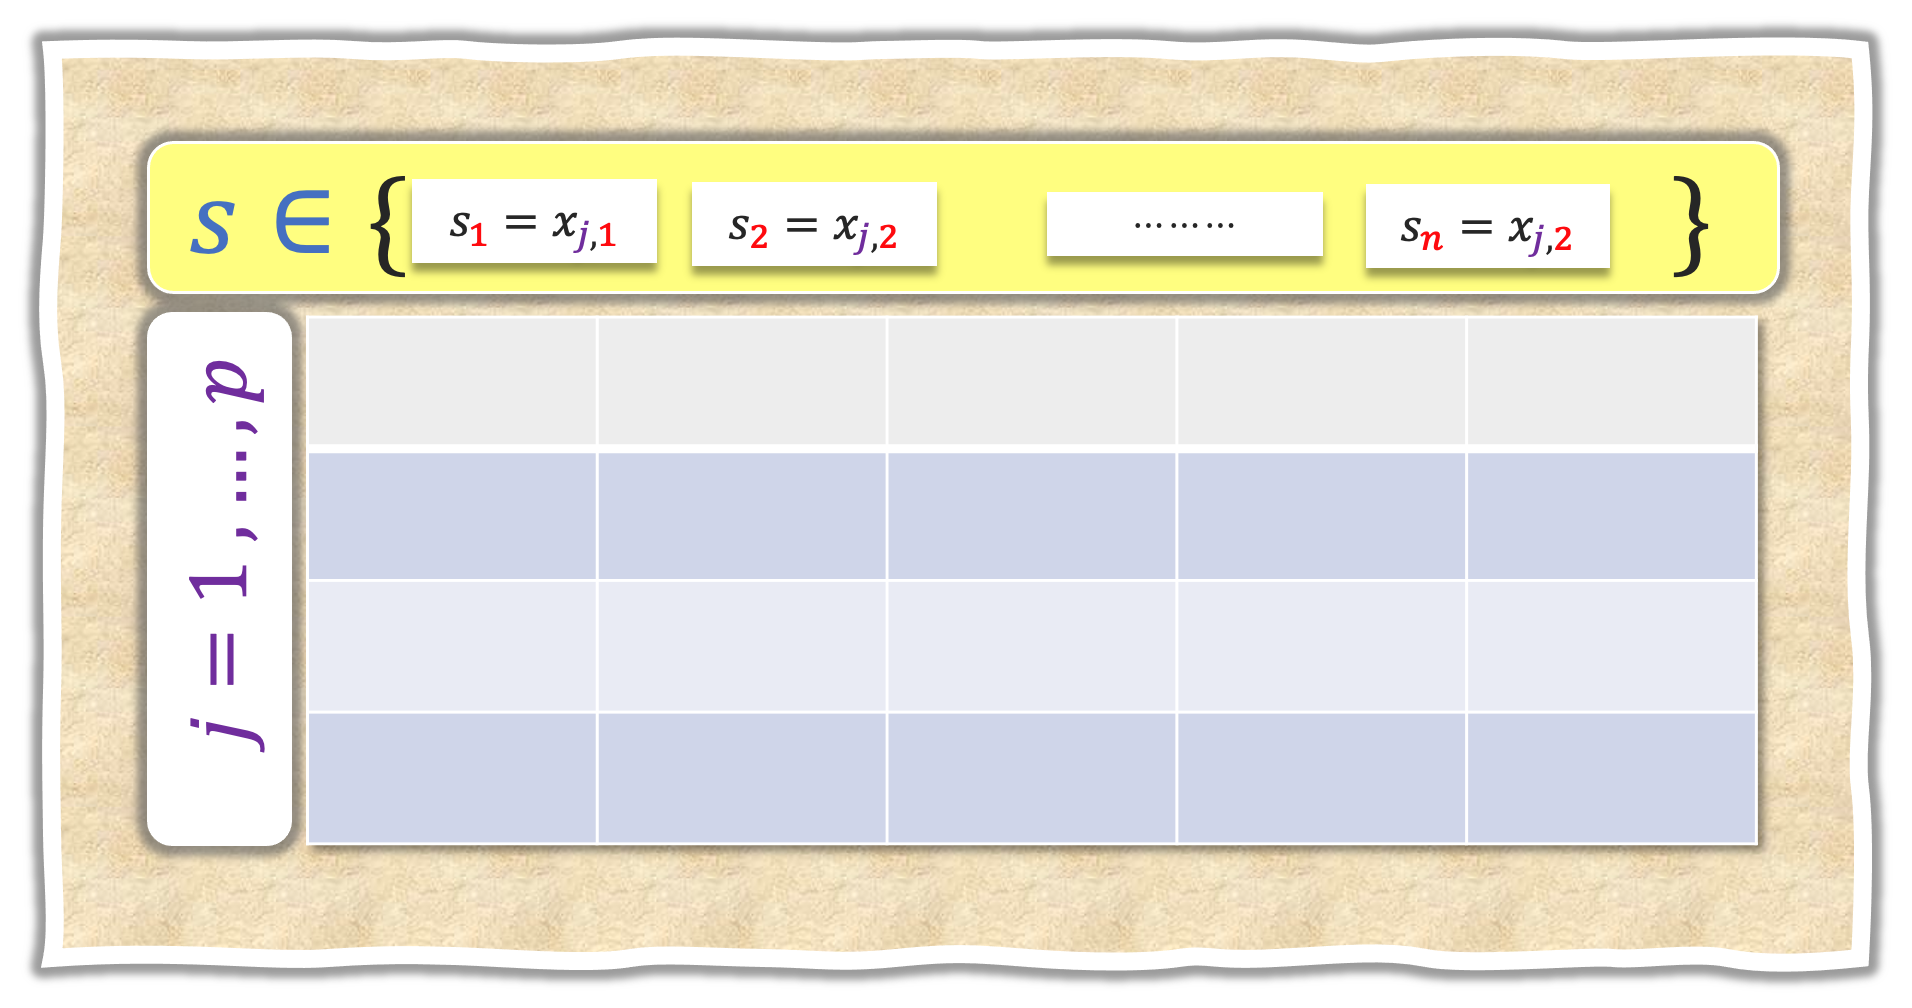
\includegraphics[scale=.35]{figs/R1_R2_table.png}
%\end{center}
%%\vspace{.1in}
%%\begin{enumerate}
%%%\qBrd[4in]{airforceblue!50}{
%%%\item[\sqBullet{bluebell}] A
%%%}
%%%\qBrd[4in]{babyblue!50}{
%%%\item[\sqBullet{babyblue}]  A
%%%}
%%\end{enumerate}
%}\\
%\vspace{.2in}
%
%\end{frame}
%
%
%
%
%\begin{frame}
%\qBrd[4.7in]{babyblueeyes!50}{
%\begin{center}
%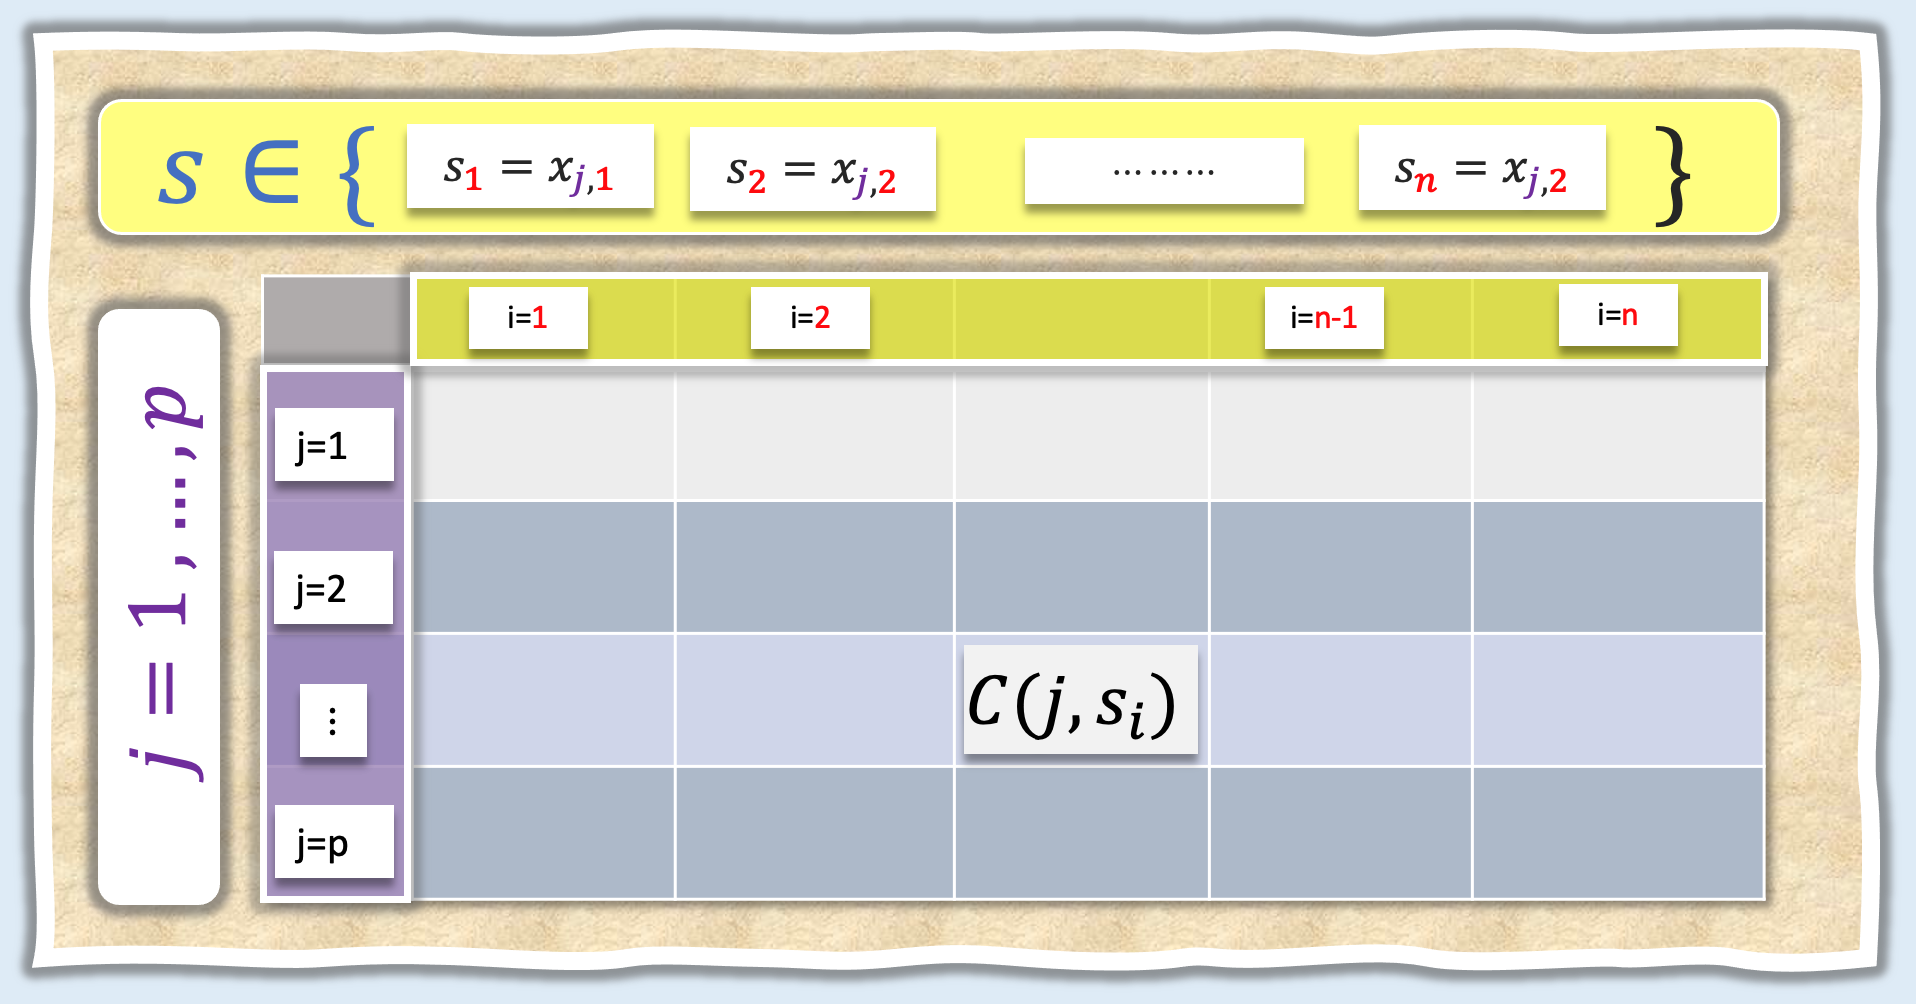
\includegraphics[scale=.35]{figs/R1_R2_table1.png}
%\end{center}
%%\vspace{.1in}
%%\begin{enumerate}
%%\qBrd[4in]{airforceblue!50}{
%%\item[\sqBullet{bluebell}] A
%%}
%%\qBrd[4in]{babyblue!50}{
%%\item[\sqBullet{babyblue}]  A
%%}
%%\end{enumerate}
%}\\
%\vspace{.8in}
%
%\end{frame}
%
%
%\subsection{An Example}
%
%\begin{frame}
%\qBrd[4.7in]{babyblueeyes!50}{
%\begin{center}
%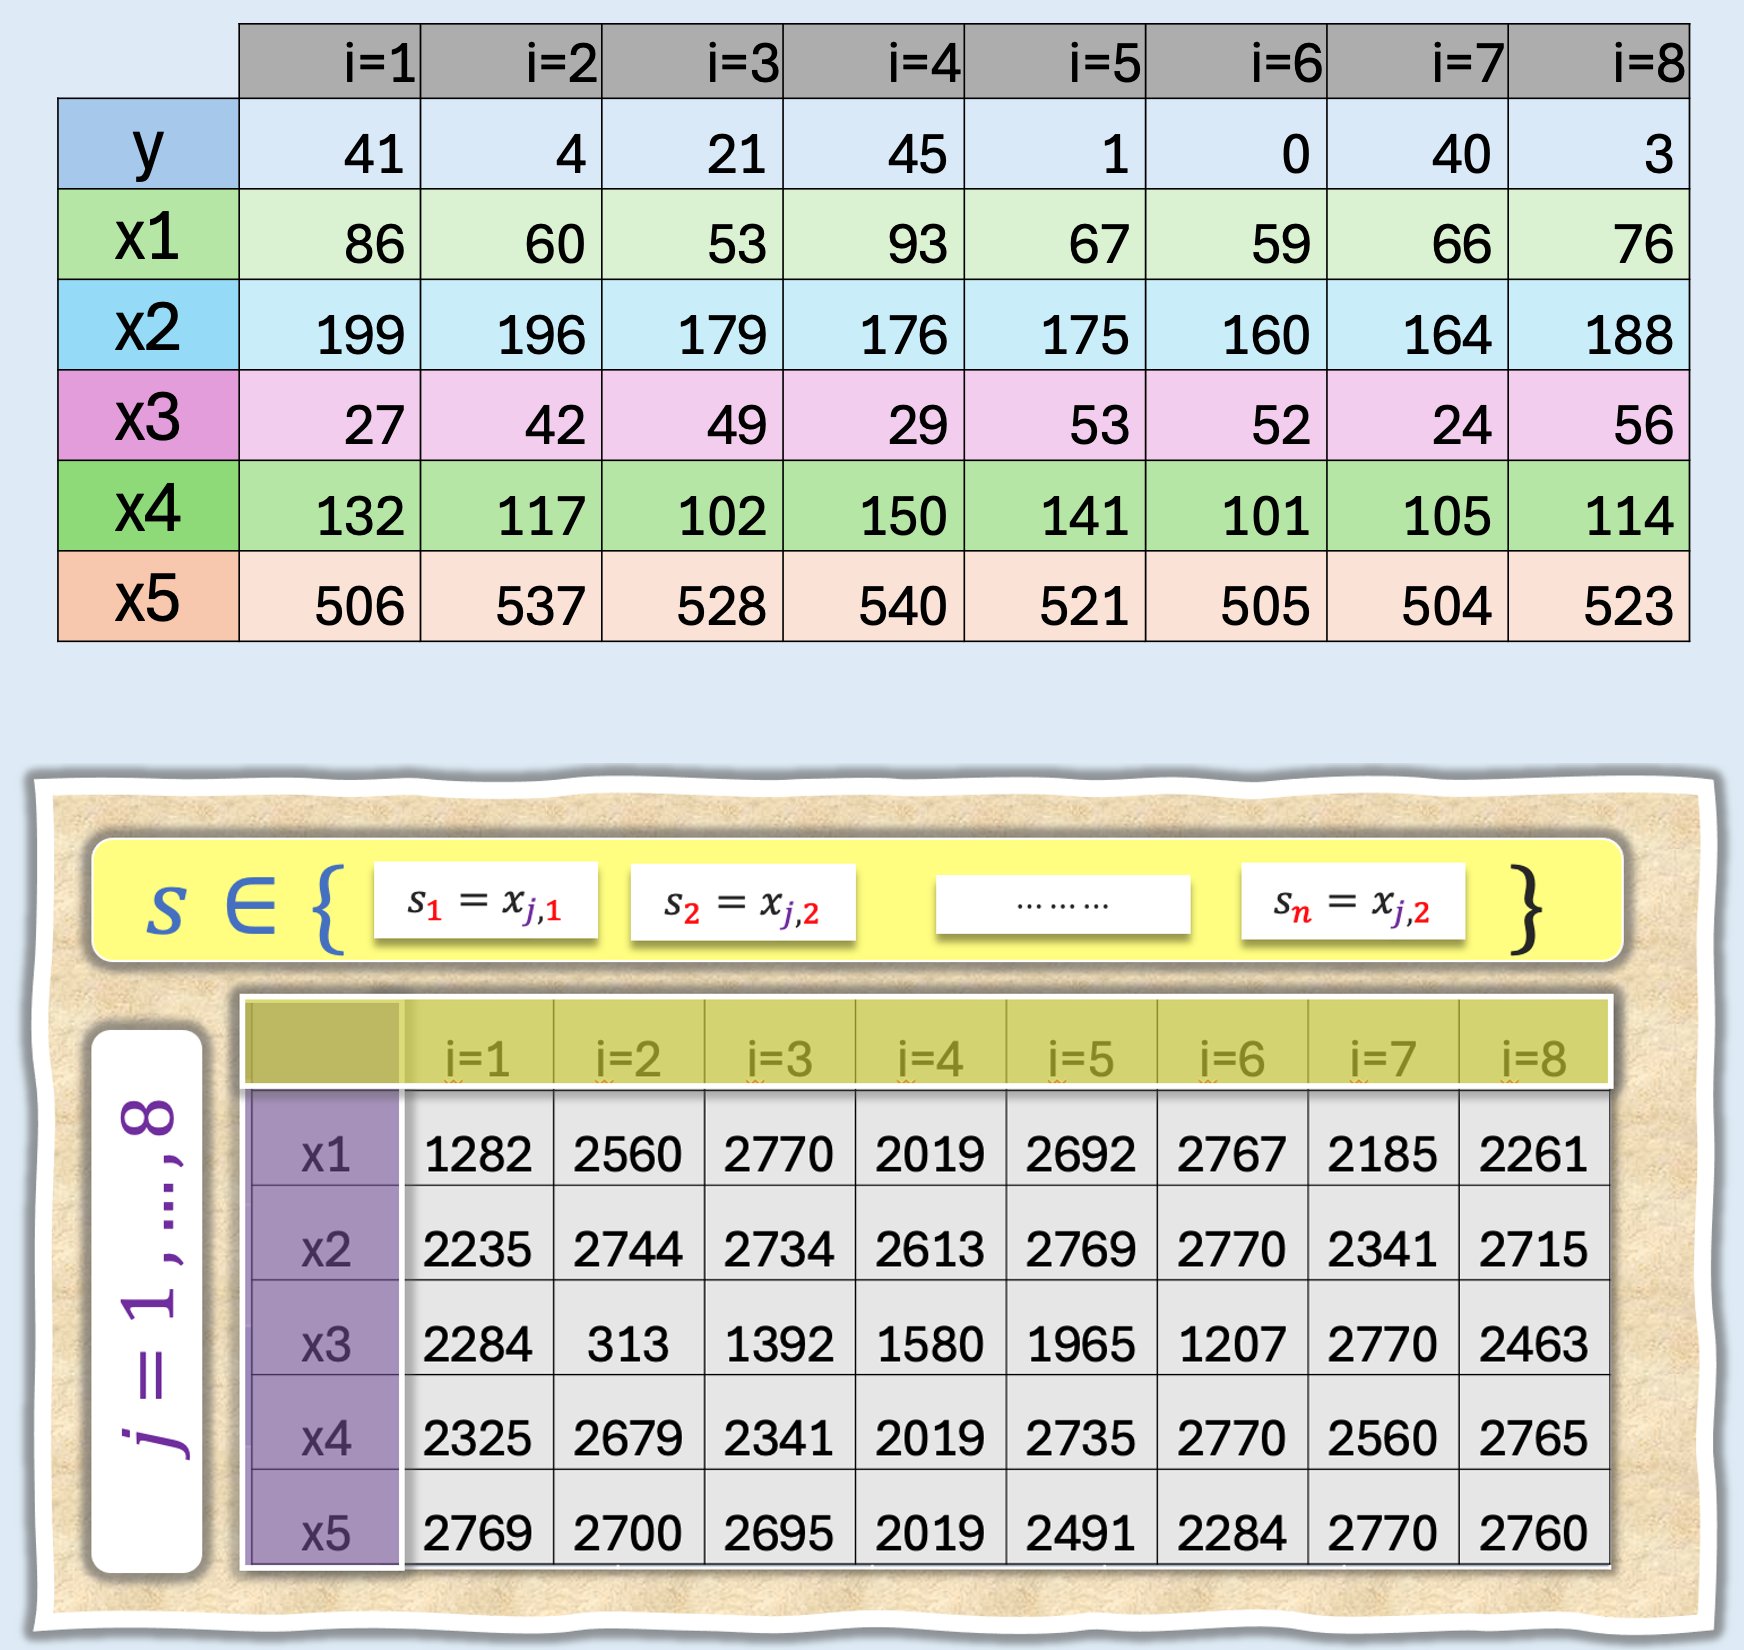
\includegraphics[scale=.28]{figs/R1_R2_table_Example.png}
%\end{center}
%%\vspace{.1in}
%%\begin{enumerate}
%%\qBrd[4in]{airforceblue!50}{
%%\item[\sqBullet{bluebell}] A
%%}
%%\qBrd[4in]{babyblue!50}{
%%\item[\sqBullet{babyblue}]  A
%%}
%%\end{enumerate}
%}\\
%\vspace{.8in}
%
%\end{frame}
%
%
%
%\begin{frame}
%\qBrd[4.7in]{babyblueeyes!50}{
%\begin{center}
%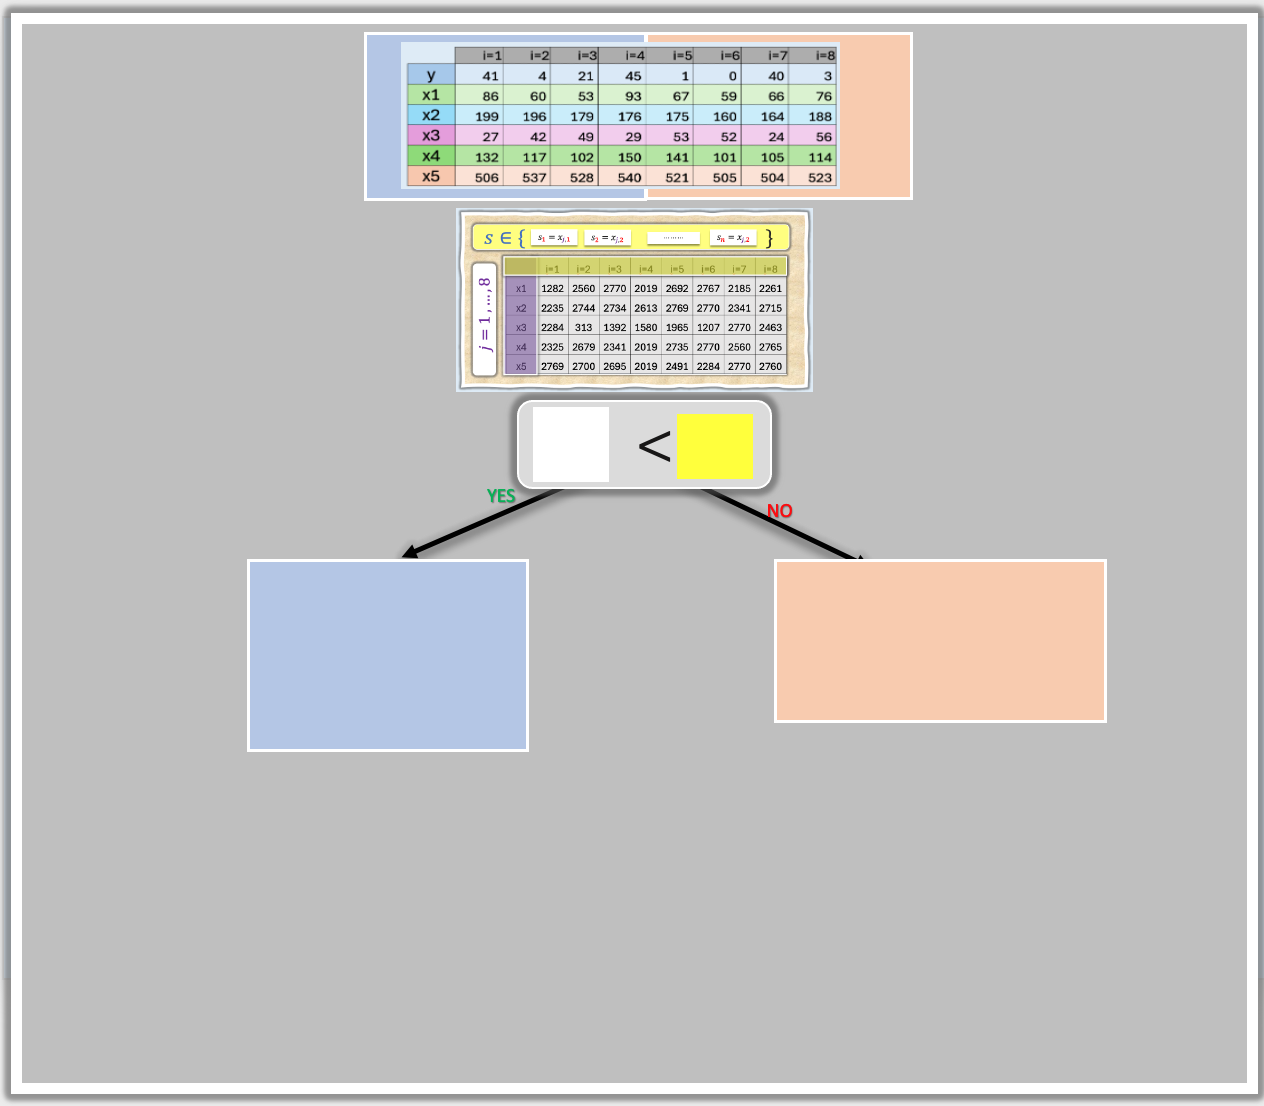
\includegraphics[scale=.4]{figs/TREE_CONSTRUCTION0.png}
%\end{center}
%}\\
%\vspace{.2in}
%
%\end{frame}
%
%
%
%
%\begin{frame}
%\qBrd[4.7in]{babyblueeyes!50}{
%\begin{center}
%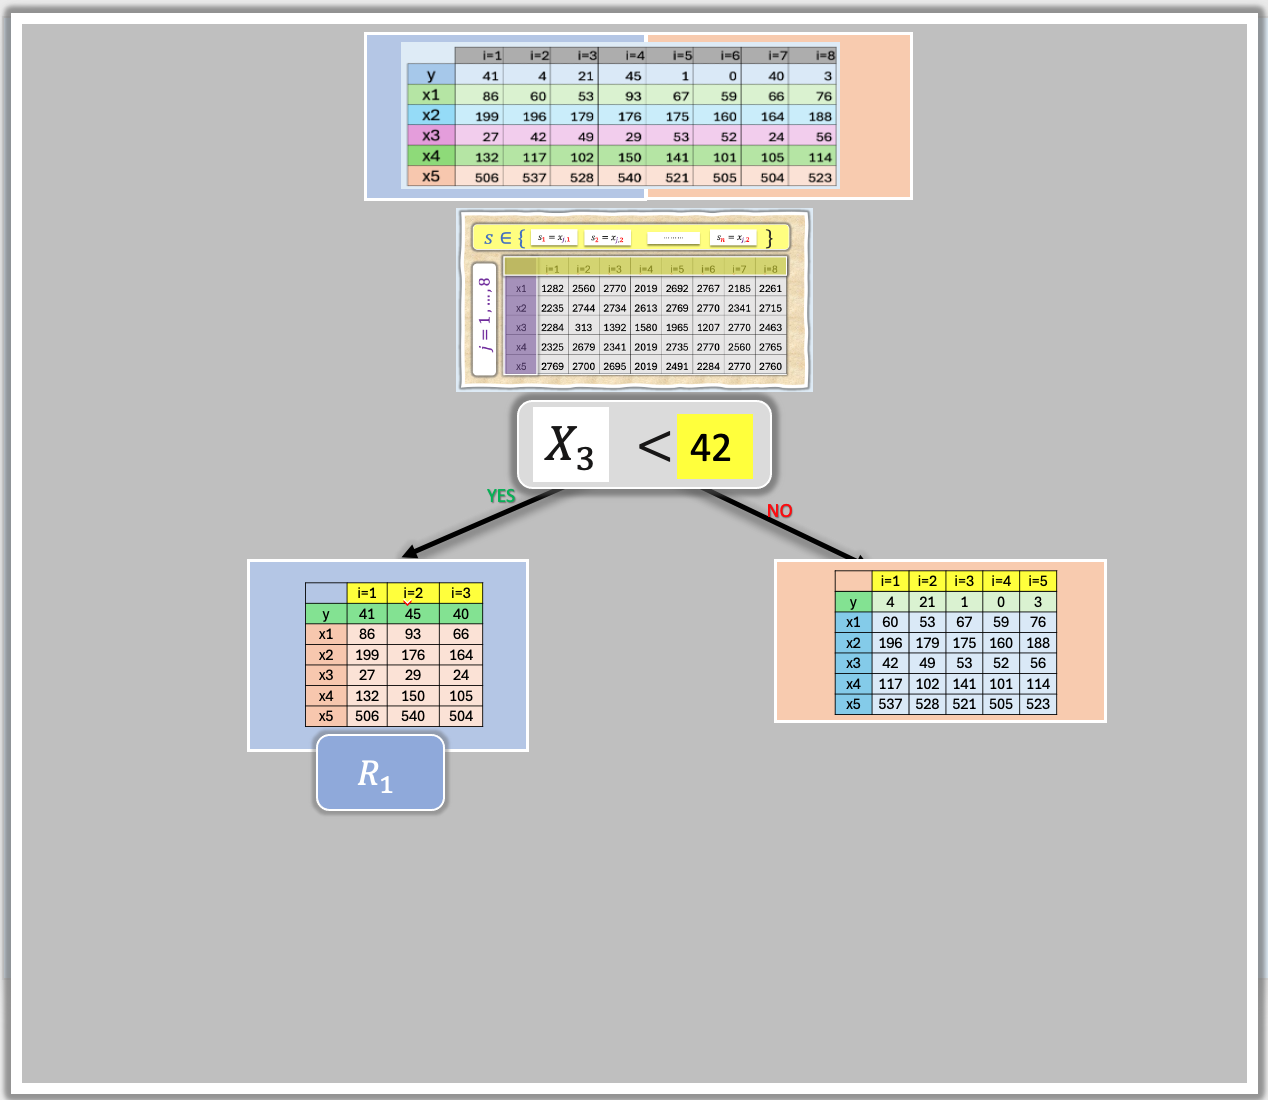
\includegraphics[scale=.4]{figs/TREE_CONSTRUCTION01.png}
%\end{center}
%}\\
%\vspace{.2in}
%
%\end{frame}
%
%
%\begin{frame}
%\qBrd[4.7in]{babyblueeyes!50}{
%\begin{center}
%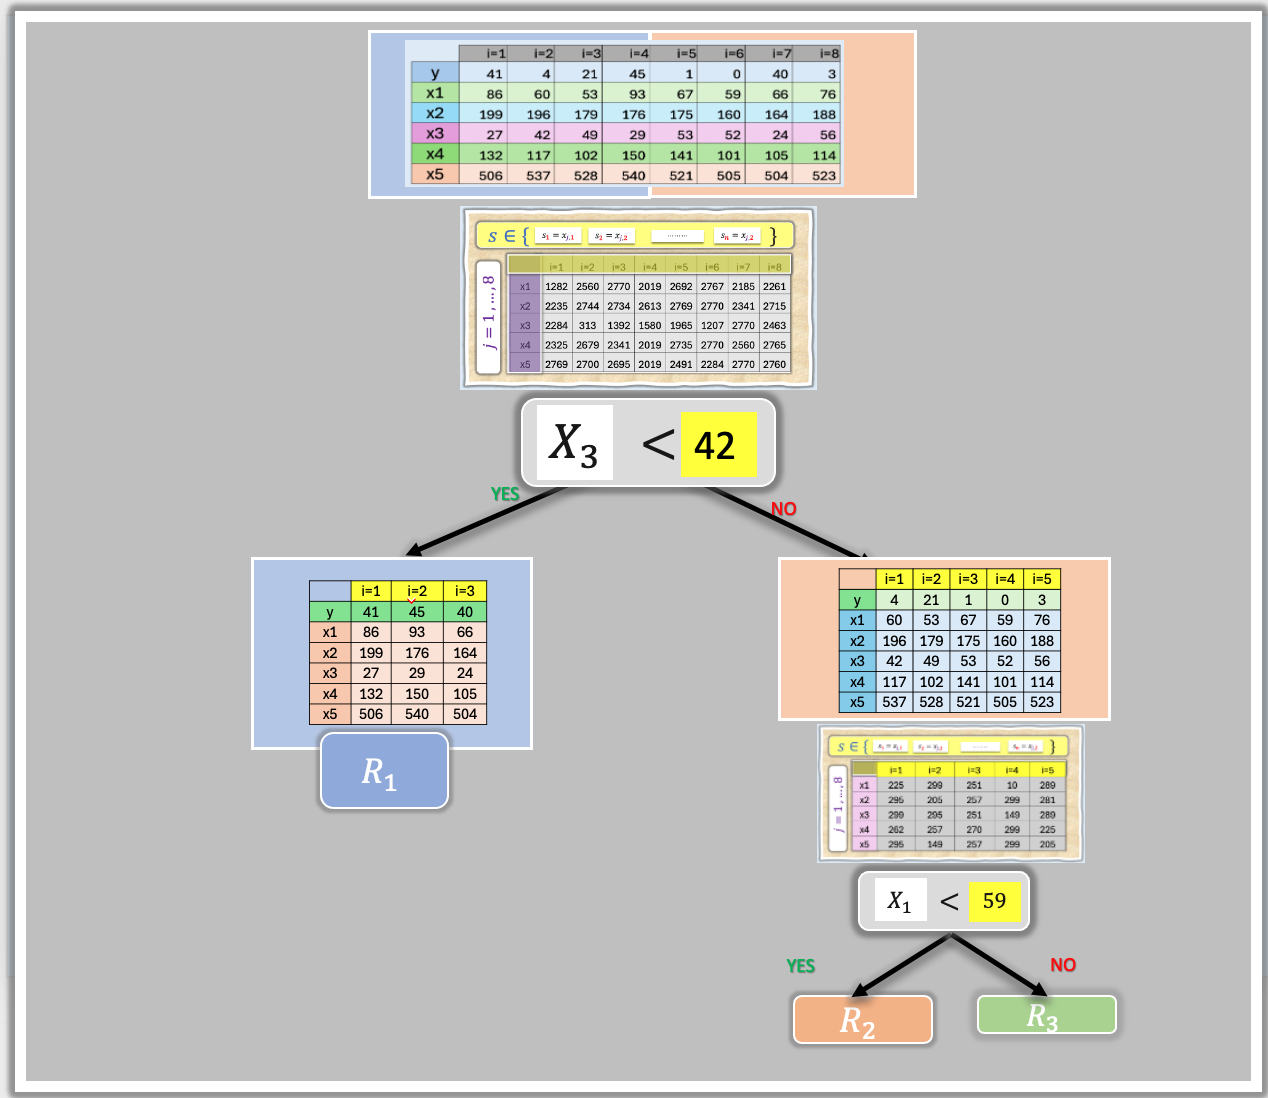
\includegraphics[scale=.4]{figs/TREE_CONSTRUCTION.png}
%\end{center}
%%\vspace{.1in}
%%\begin{enumerate}
%%\qBrd[4in]{airforceblue!50}{
%%\item[\sqBullet{bluebell}] A
%%}
%%\qBrd[4in]{babyblue!50}{
%%\item[\sqBullet{babyblue}]  A
%%}
%%\end{enumerate}
%}\\
%\vspace{.2in}
%
%\end{frame}
%
%
%
%
%
%{ \setbeamercolor{background canvas}{bg=}
%\includepdf[pages={18-19}, scale=1]{STAT380-Unit4.pdf}
%}
%
%
%
%
%
%
%
%\TransitionFrame[antiquebrass]{\Large Tree, Subtree,  and Tree Pruning }
%%
%
%
%
%
%
%\TransitionFrame[olive]{\Large Subtree }
%%
%
%
%
%
%\begin{frame}
%\qBrd[4.7in]{babyblueeyes!50}{
%\vspace{-.2in}
%\begin{center}
%\qBrd[.3in]{babyblueeyes}{$\;\HLTW{T_0}$}
%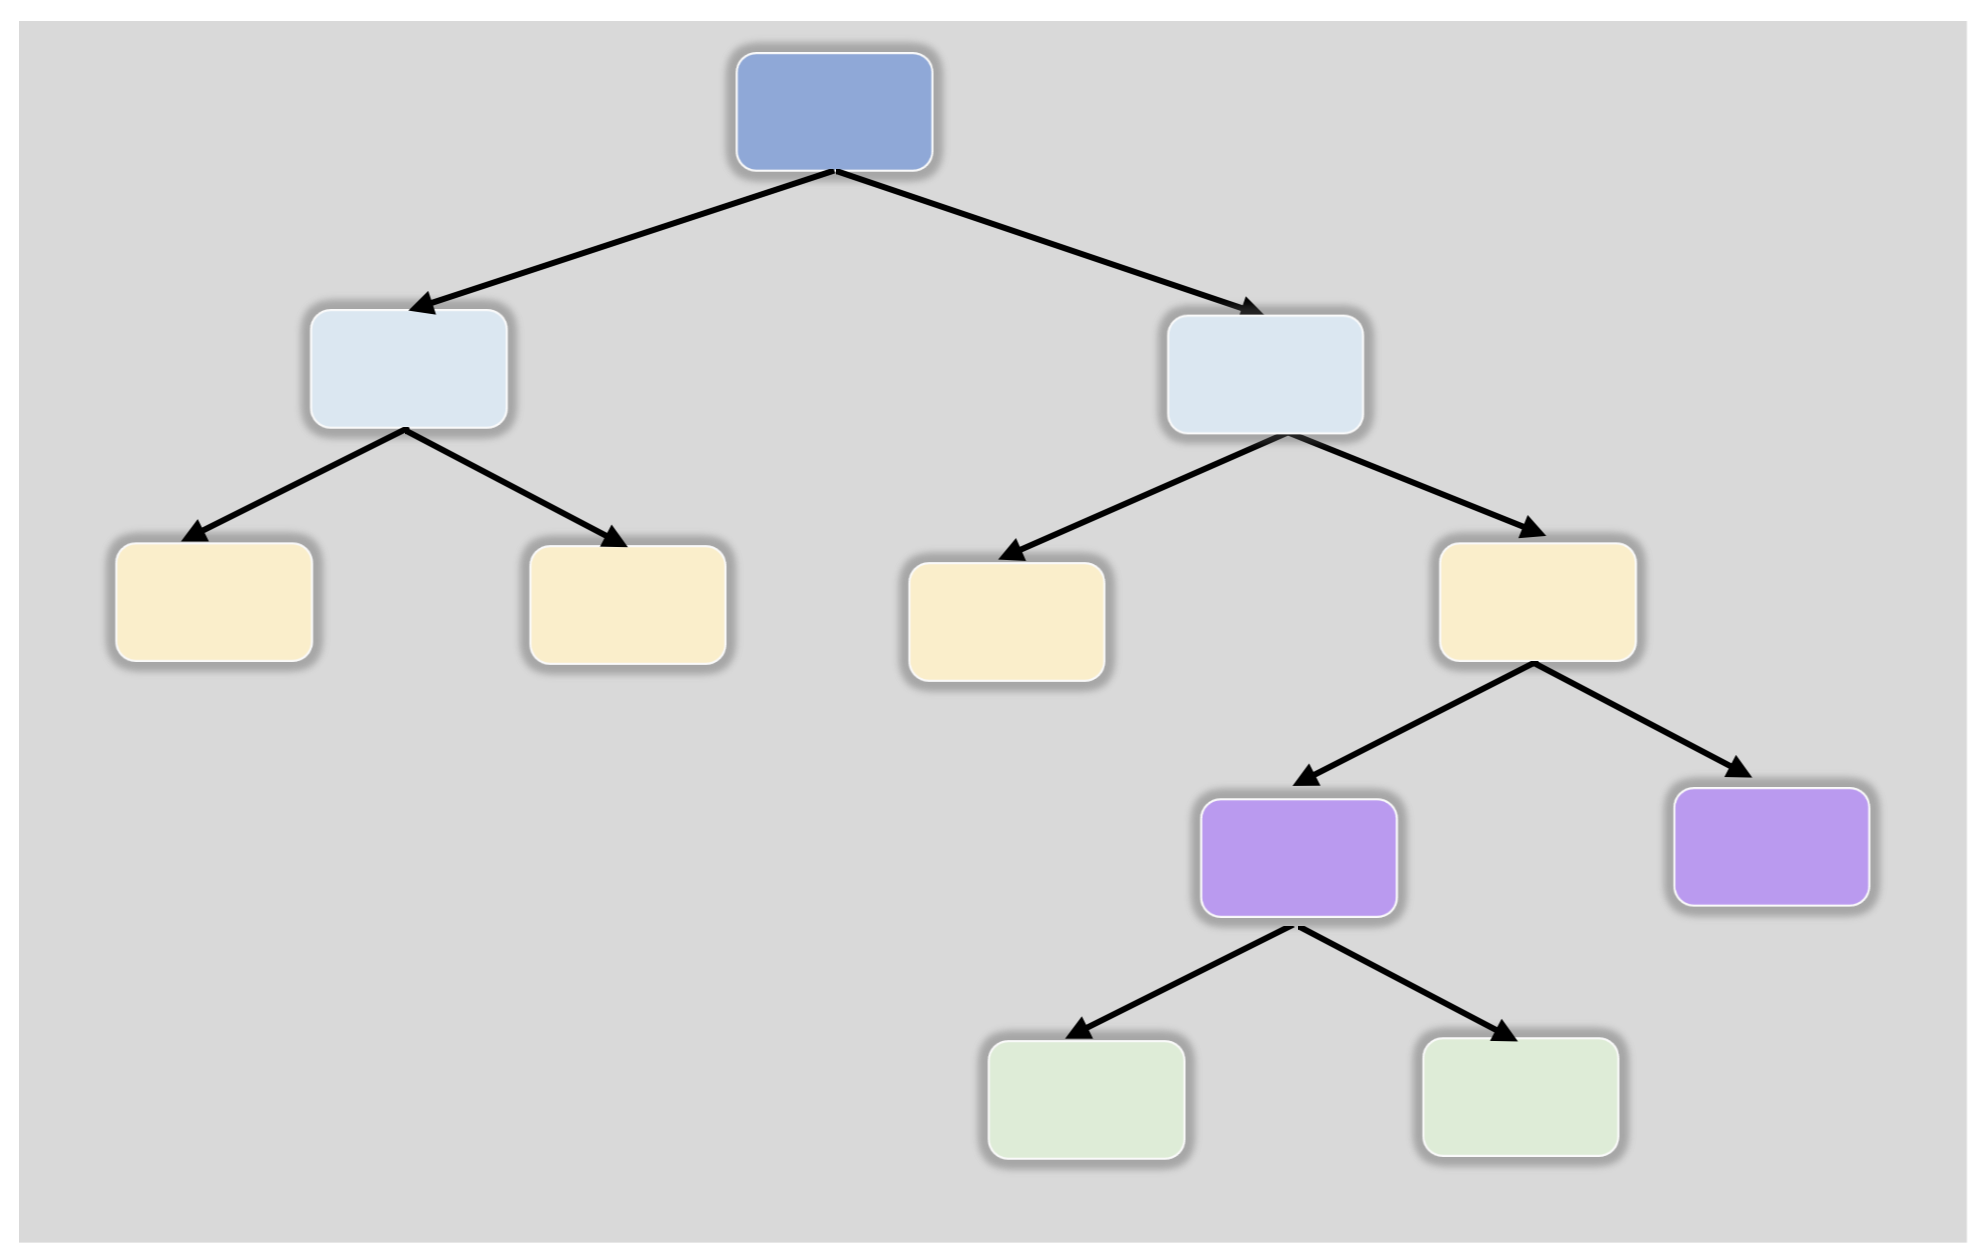
\includegraphics[scale=.32]{figs/T0.png}
%\end{center}
%}\\
%\end{frame}
%
%
%
%\begin{frame}
%\qBrd[4.7in]{babyblueeyes!50}{
%\begin{center}
%$\Col{
%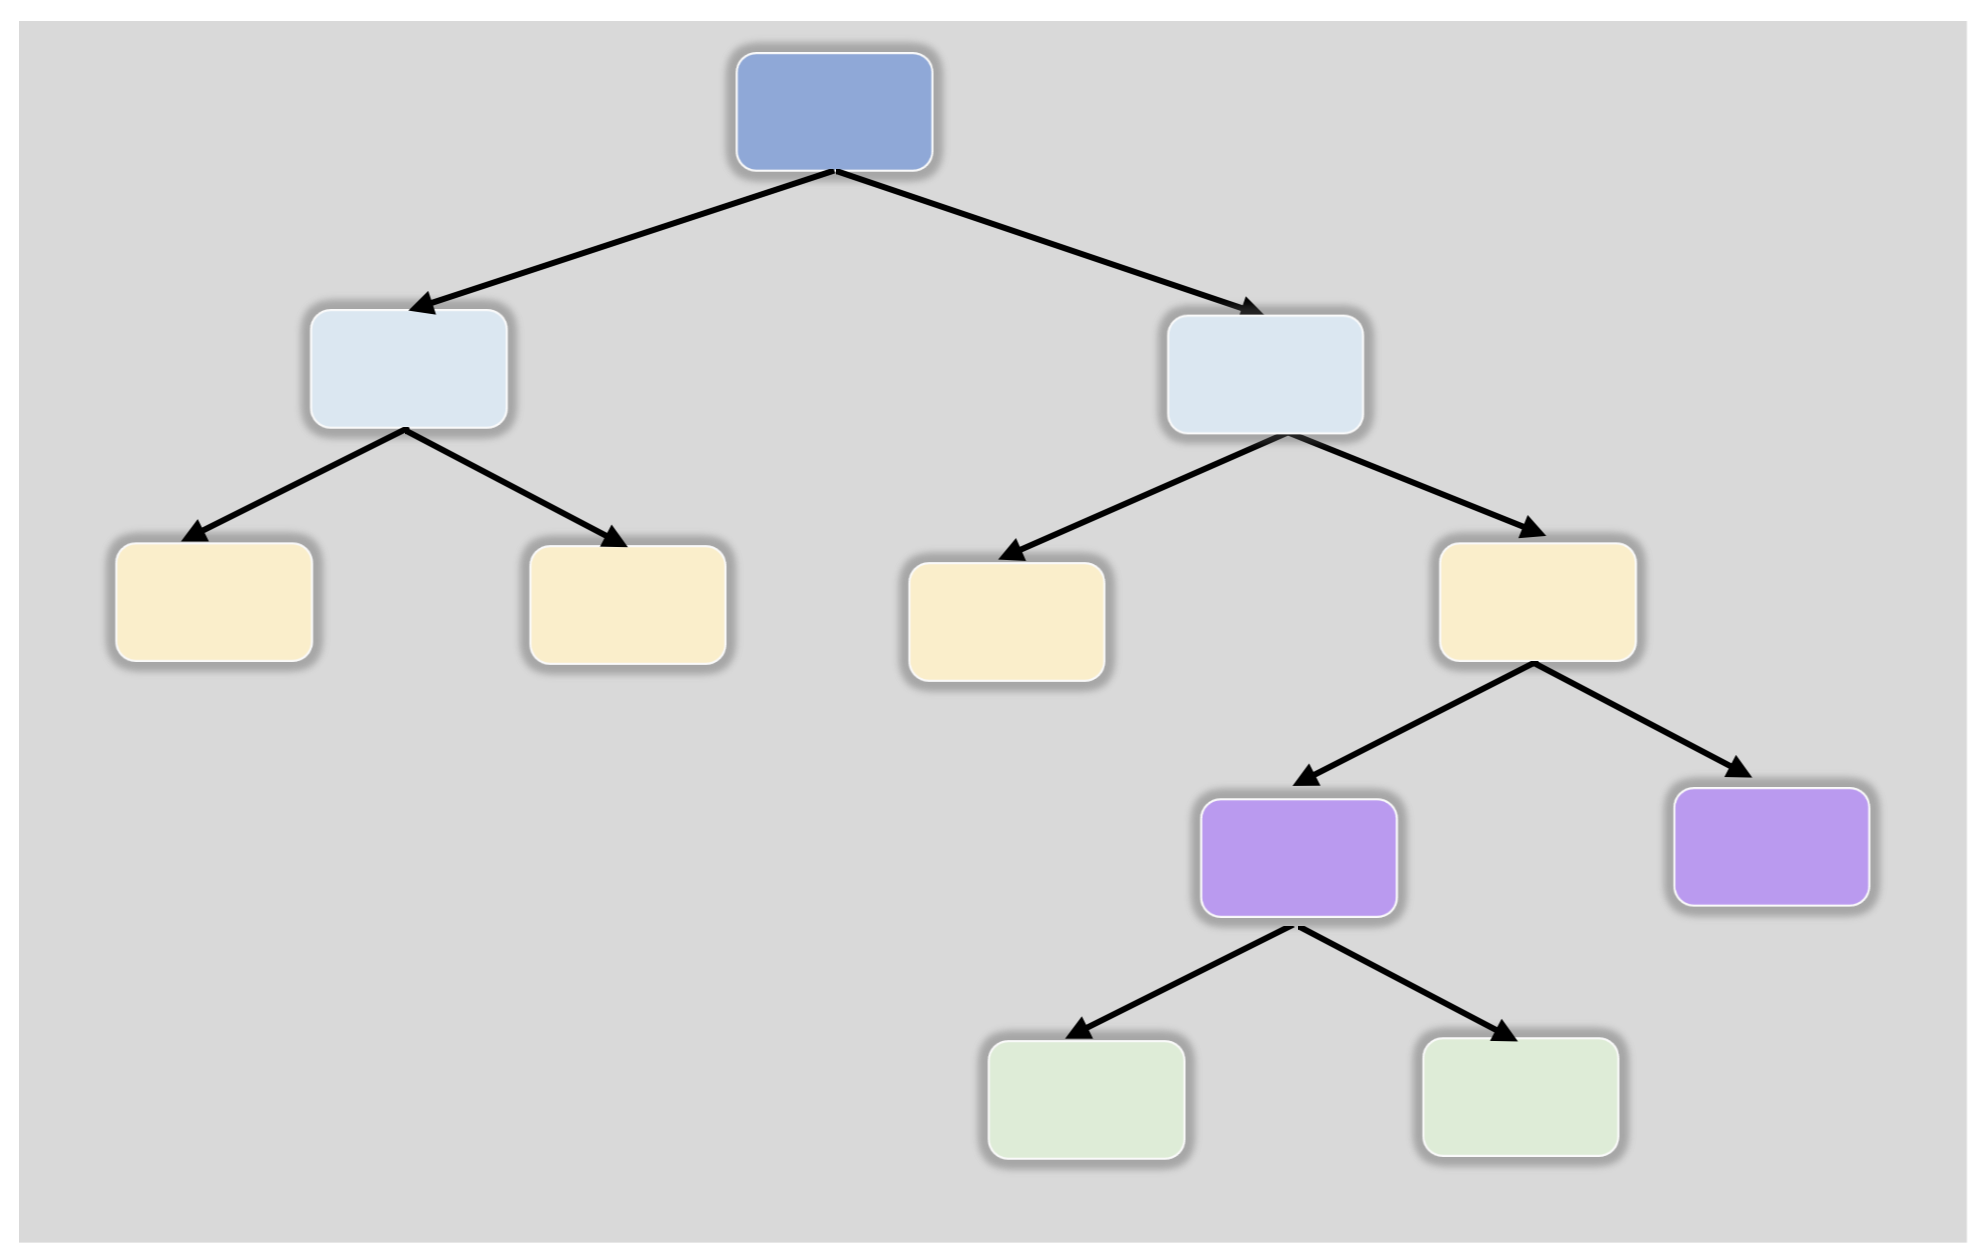
\includegraphics[scale=.15]{figs/T0.png},
%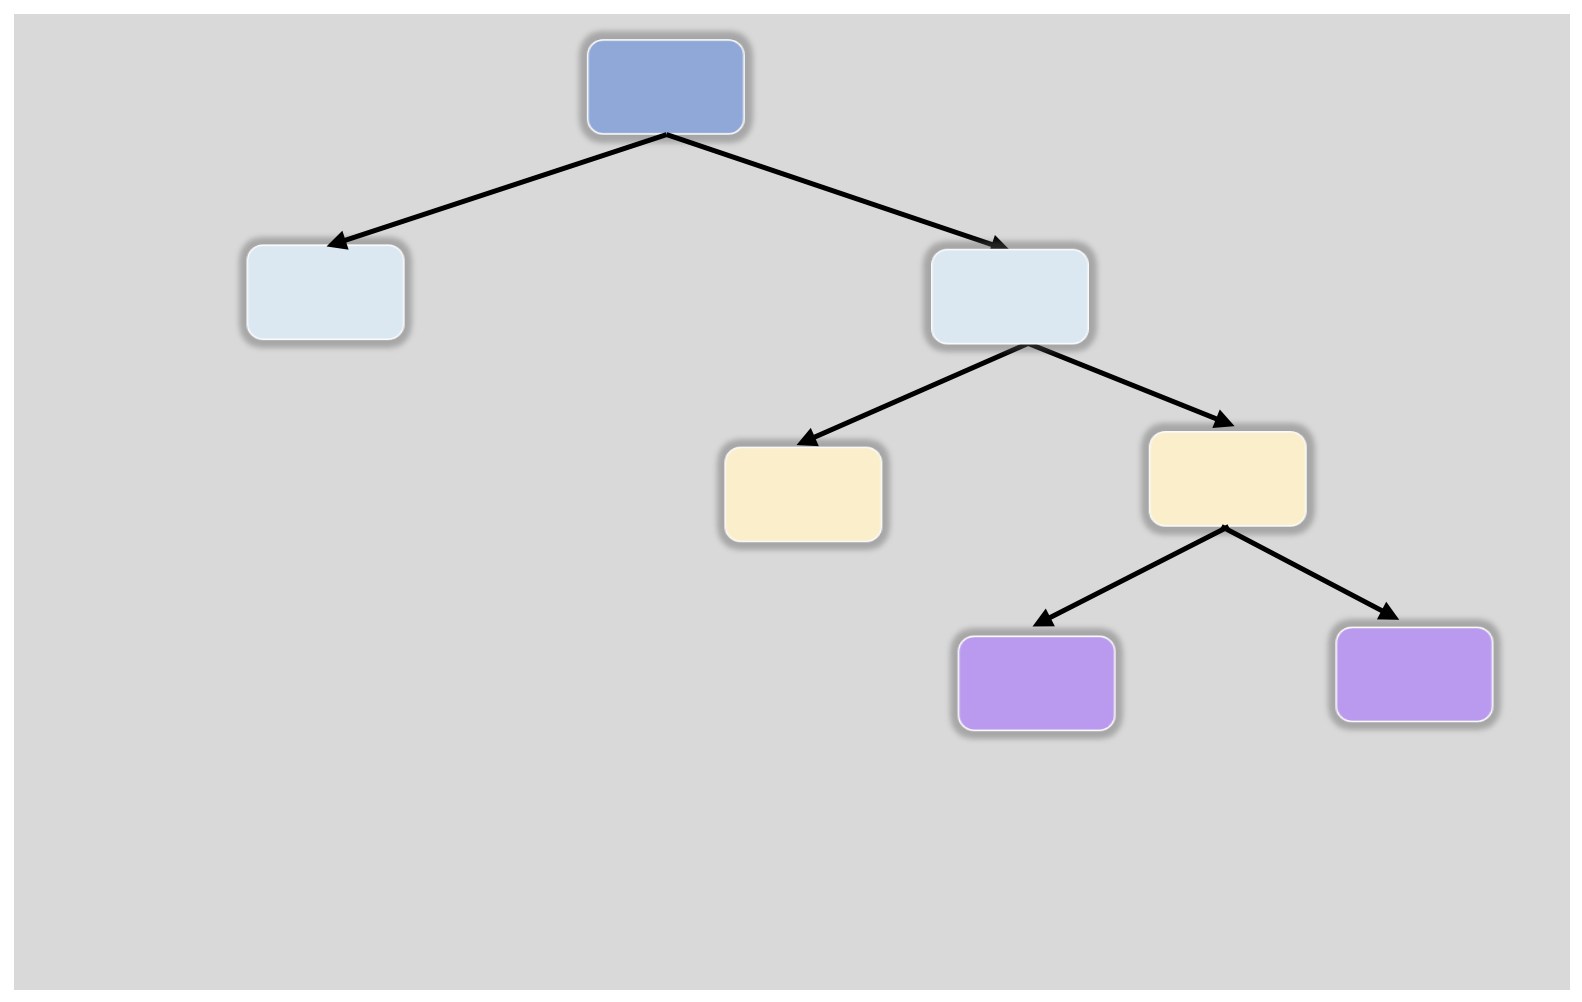
\includegraphics[scale=.28]{figs/T1.png}}$
%\end{center}
%}\\
%\end{frame}
%
%
%
%
%
%
%\begin{frame}
%\qBrd[4.7in]{babyblueeyes!50}{
%\begin{center}
%$\Col{
%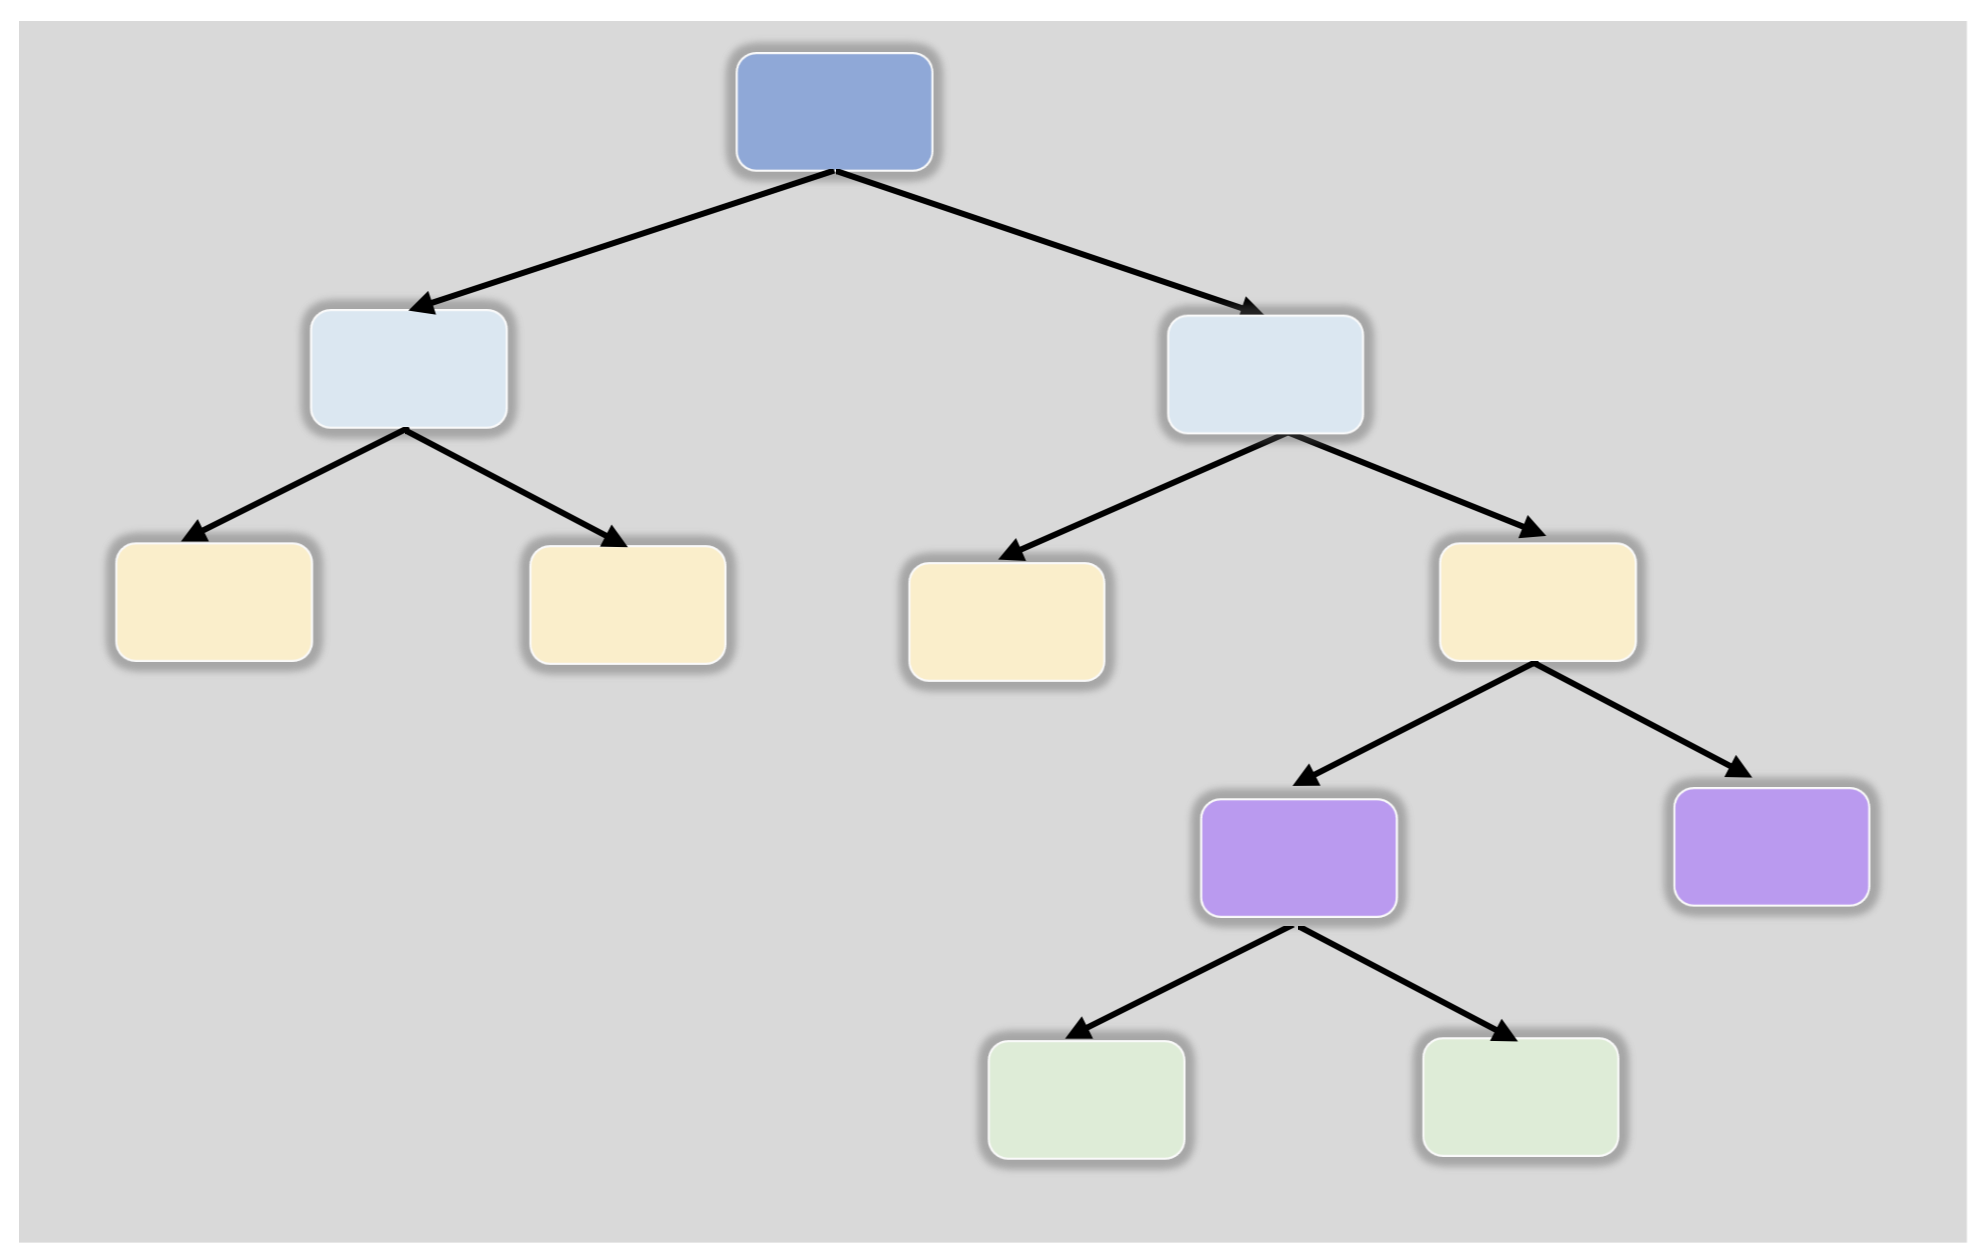
\includegraphics[scale=.15]{figs/T0.png},
%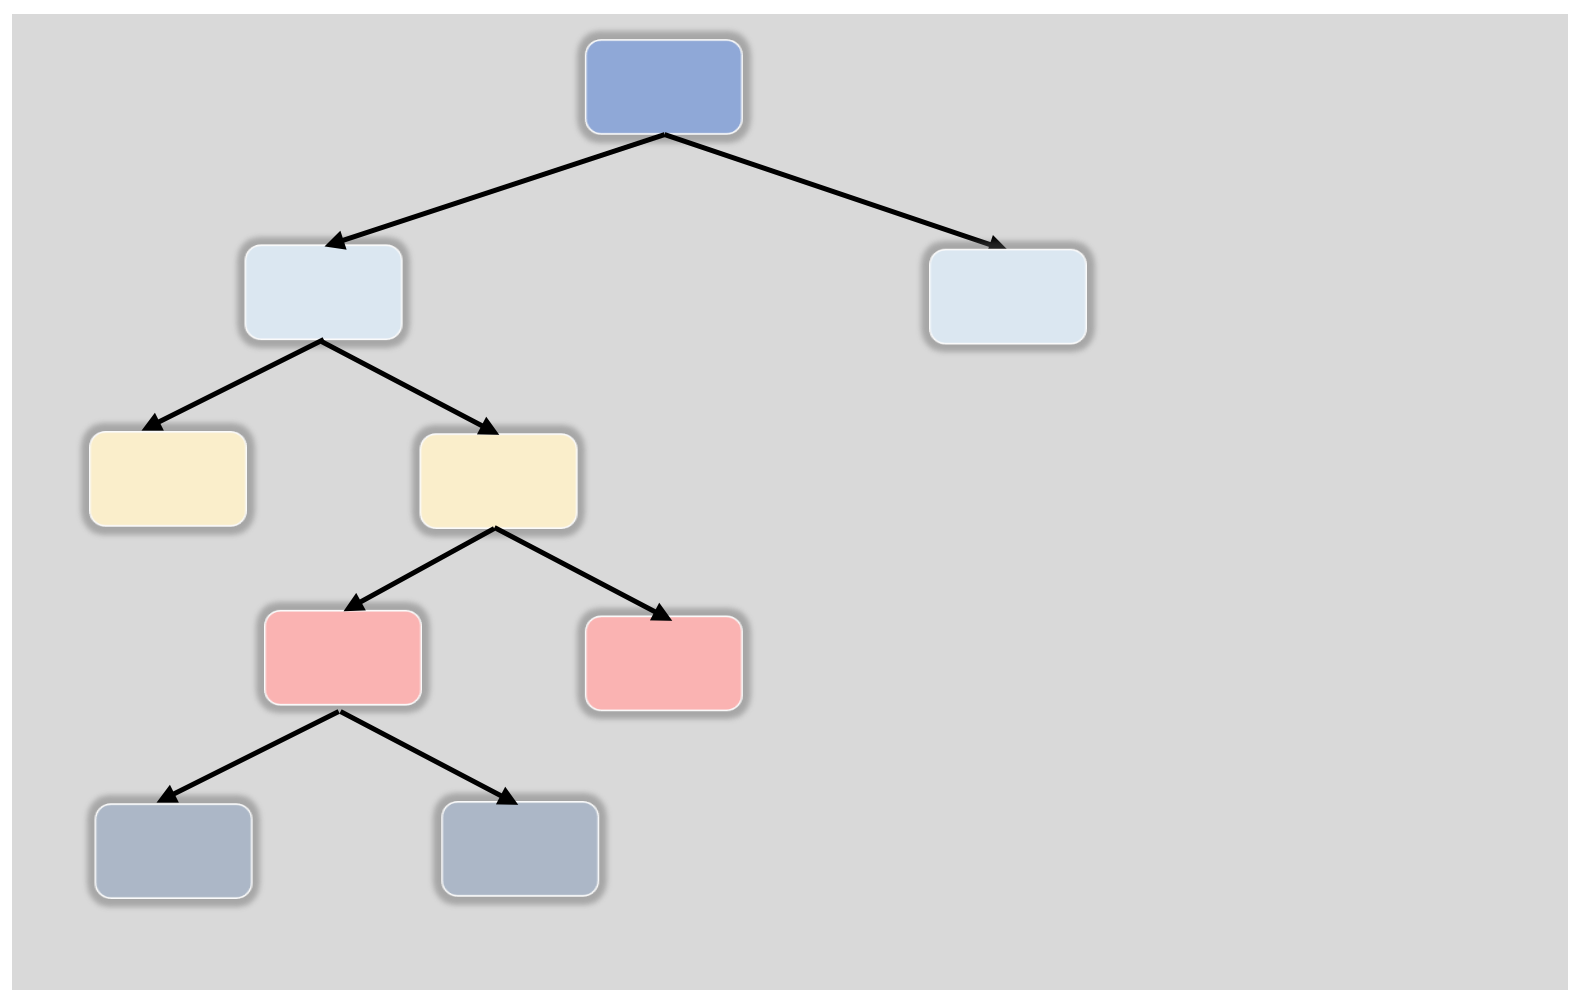
\includegraphics[scale=.28]{figs/T3.png}}$
%\end{center}
%}\\
%\end{frame}
%
%
%
%\begin{frame}
%\qBrd[4.7in]{babyblueeyes!50}{
%\begin{center}
%$\Col{
%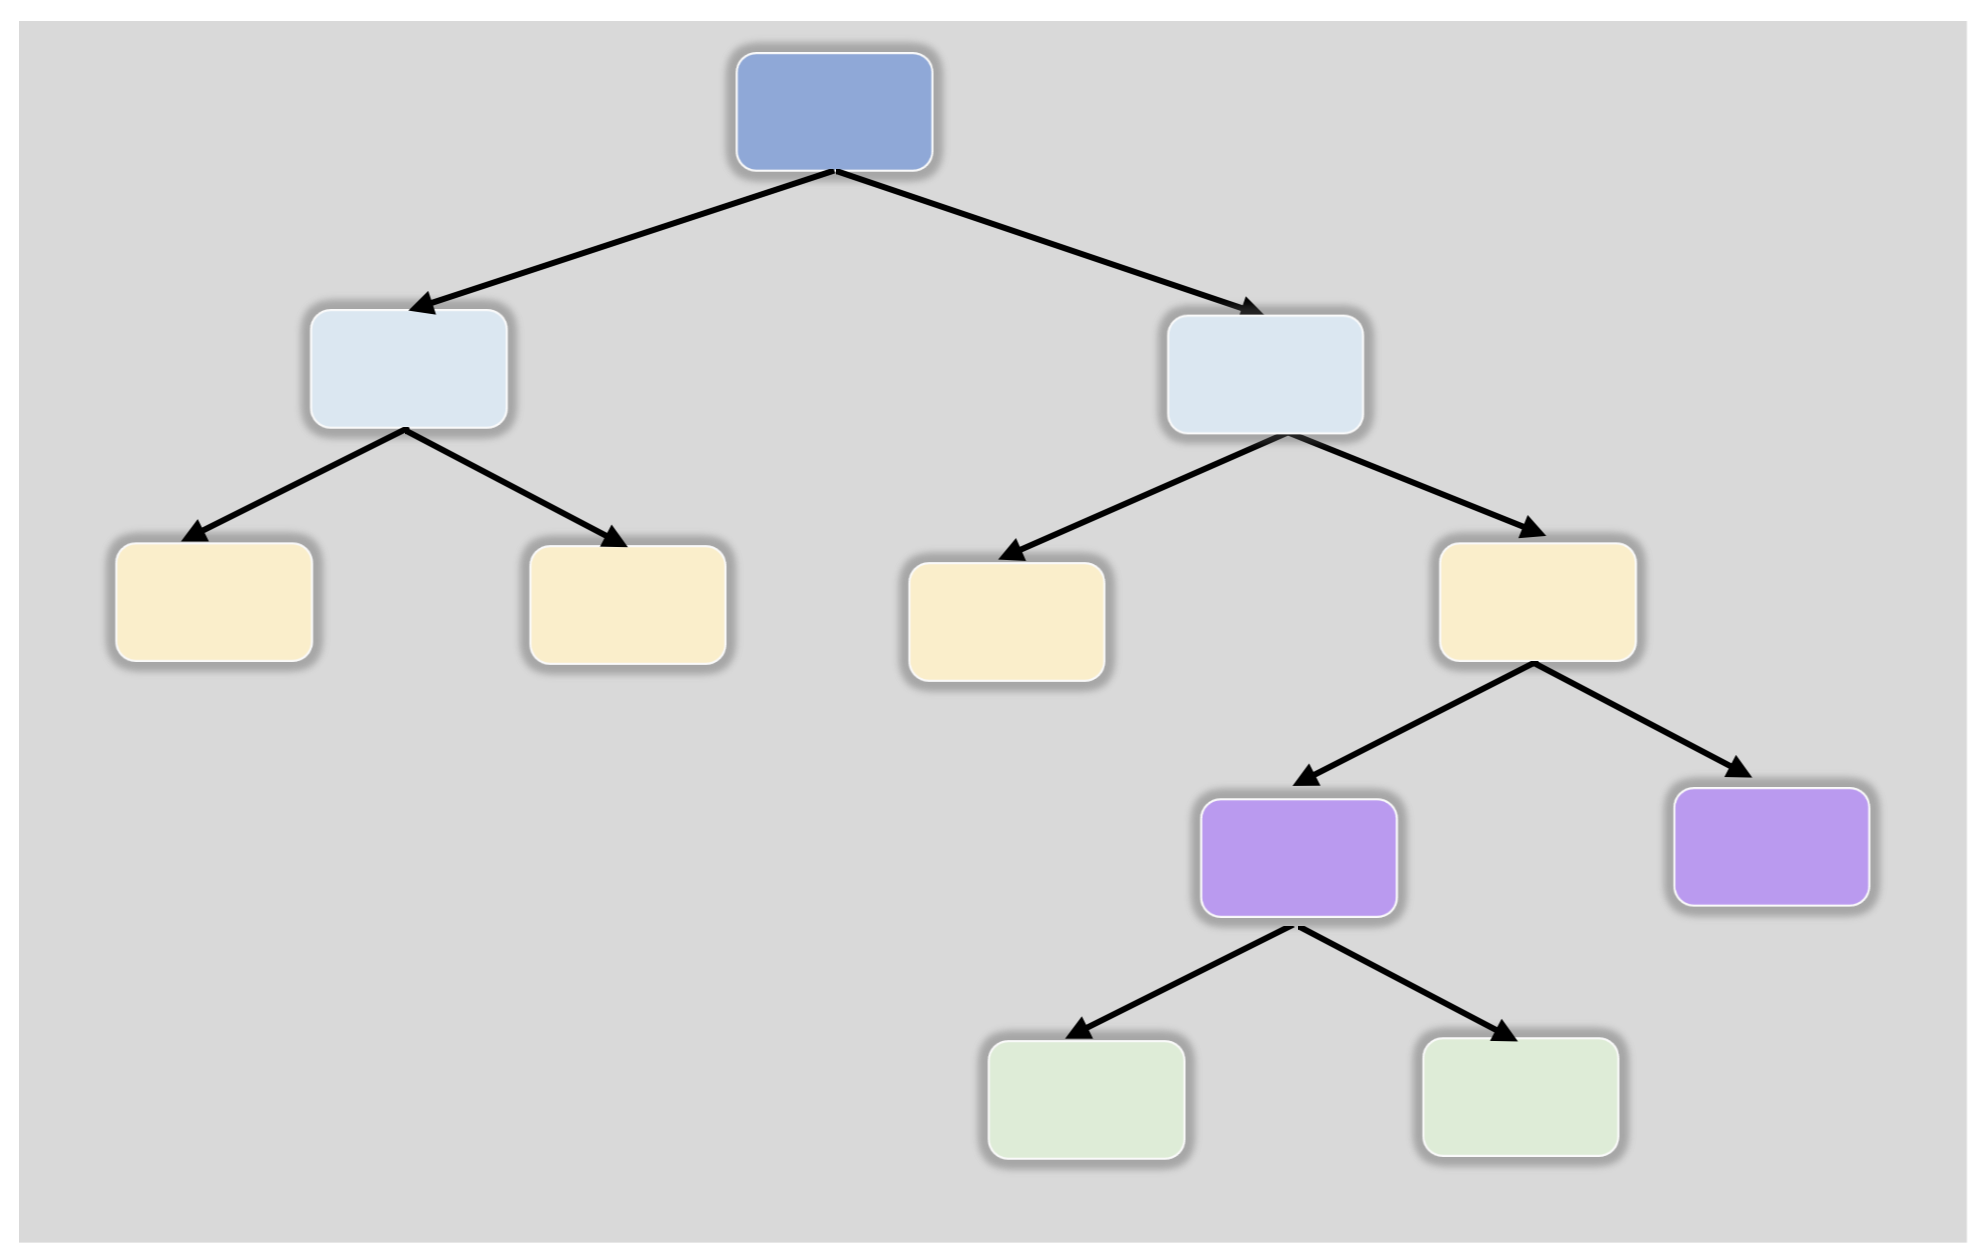
\includegraphics[scale=.15]{figs/T0.png},
%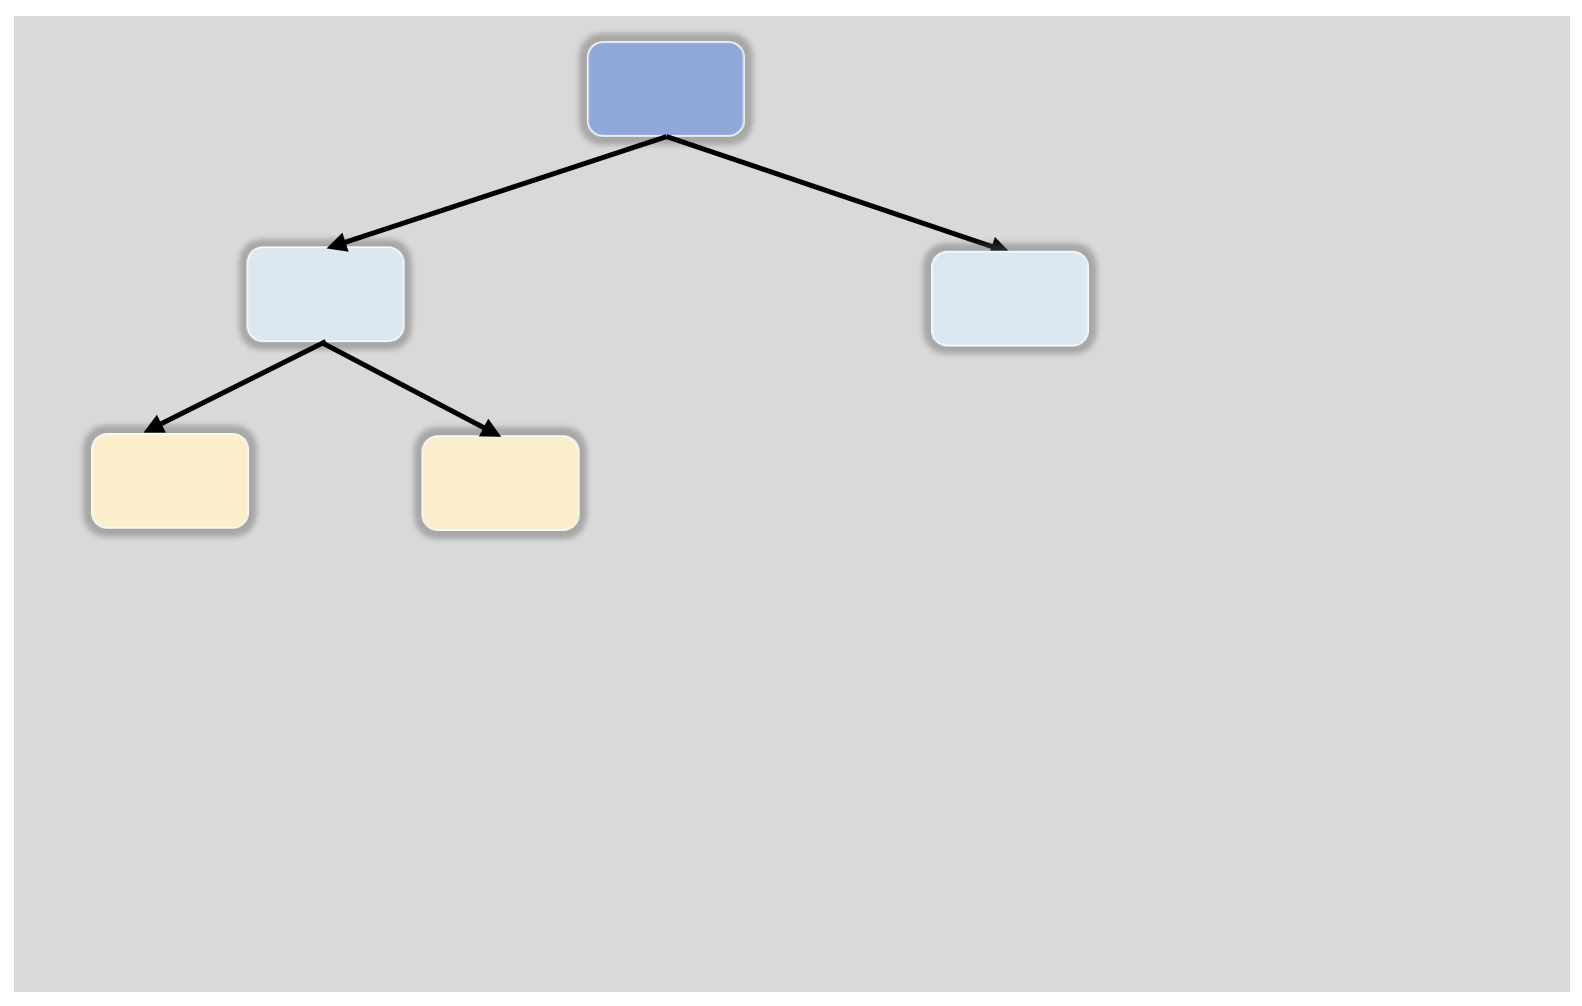
\includegraphics[scale=.28]{figs/T2.png}}$
%\end{center}
%}\\
%\end{frame}
%
%\TransitionFrame[olive]{\Large $\vert T \vert $: Order of a Tree  }
%
%
%\begin{frame}
%\qBrd[4.7in]{babyblueeyes!50}{
%\begin{center}
%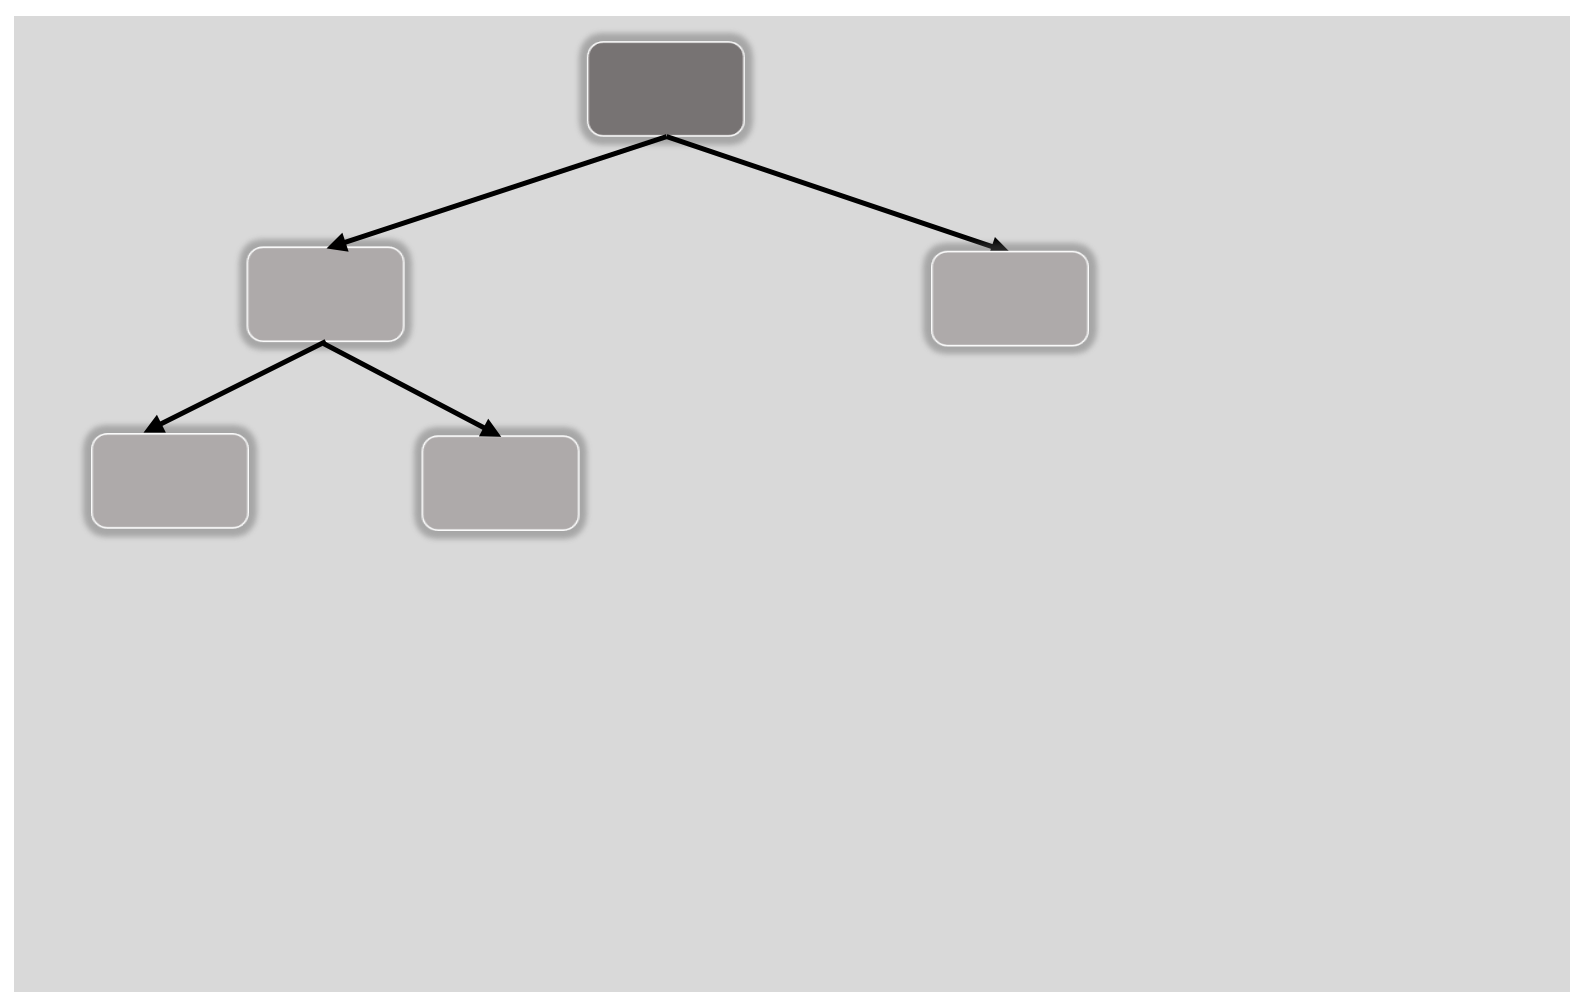
\includegraphics[scale=.4]{figs/T11_Q.png}
%\end{center}
%}\\
%\end{frame}
%
%
%\begin{frame}
%\qBrd[4.7in]{babyblueeyes!50}{
%\begin{center}
%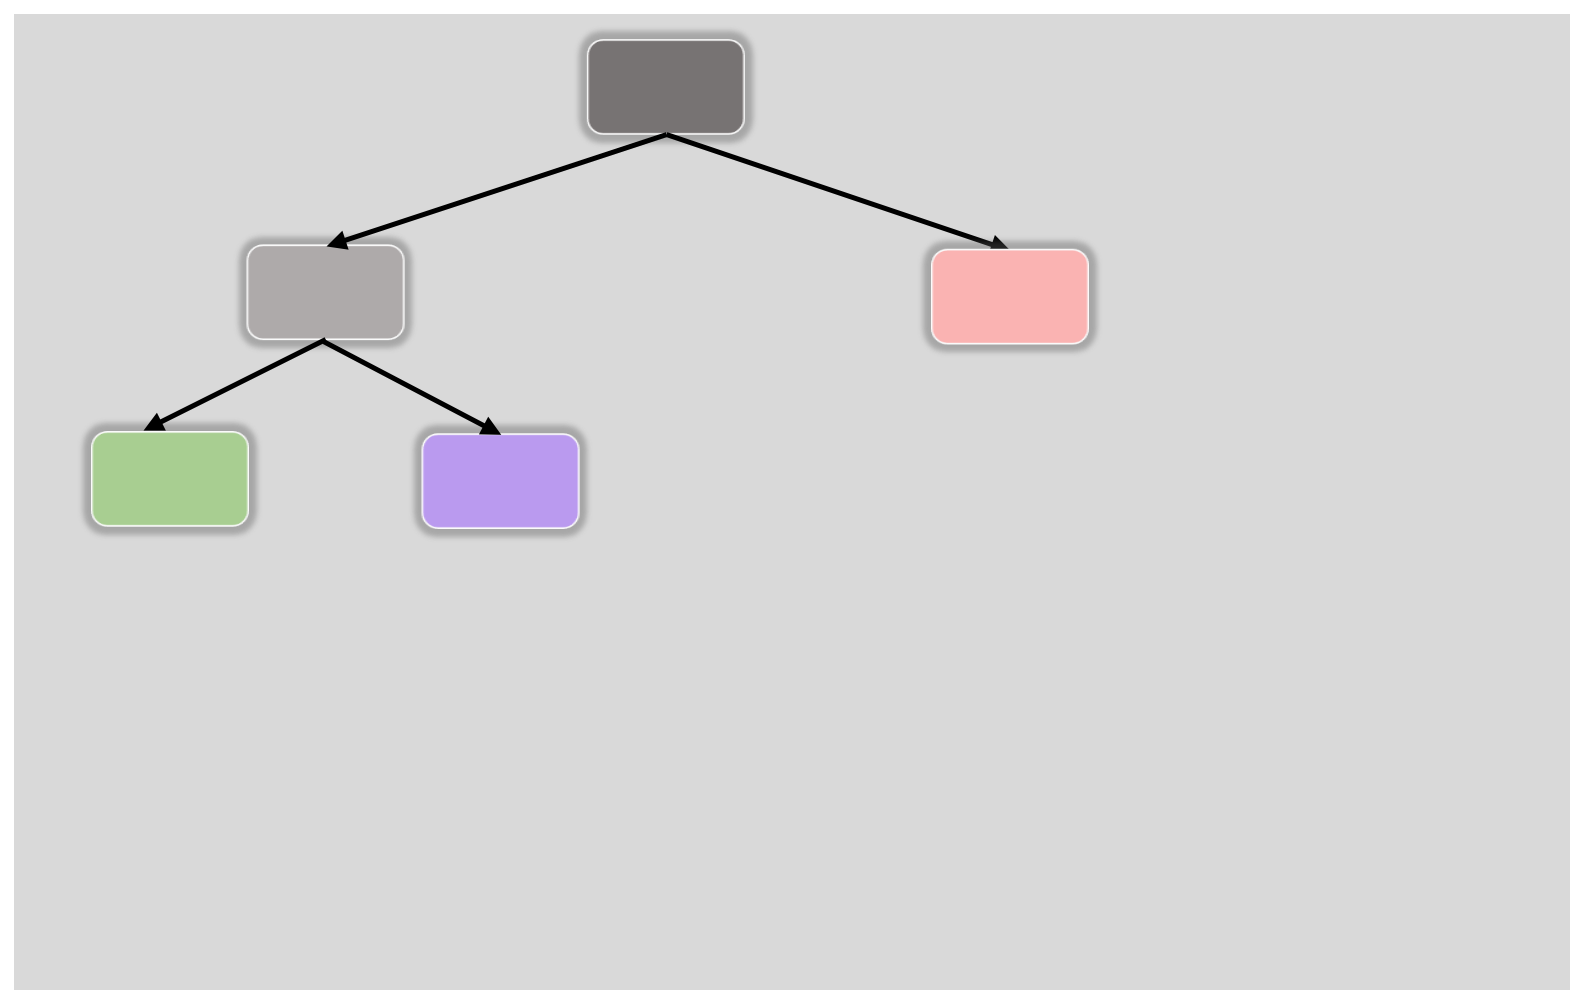
\includegraphics[scale=.4]{figs/T11_A.png}
%\end{center}
%}\\
%\end{frame}
%
%
%
%
%
%
%\begin{frame}
%\qBrd[4.7in]{babyblueeyes!50}{
%\begin{center}
%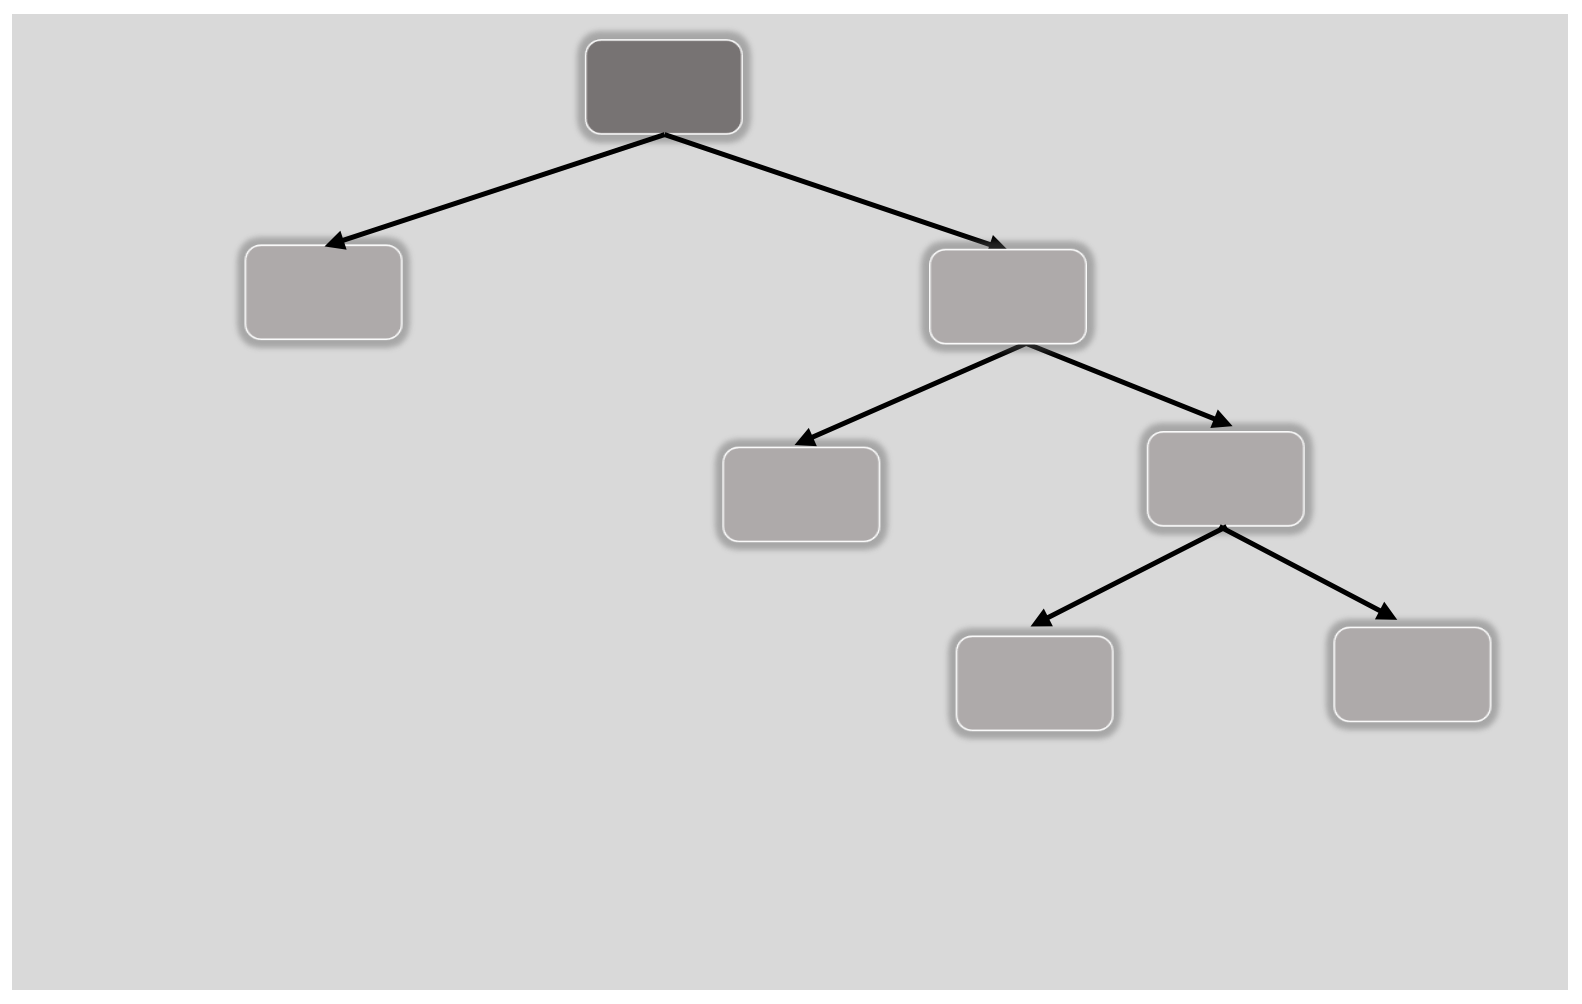
\includegraphics[scale=.4]{figs/T12_Q.png}
%\end{center}
%}\\
%\end{frame}
%
%
%\begin{frame}
%\qBrd[4.7in]{babyblueeyes!50}{
%\begin{center}
%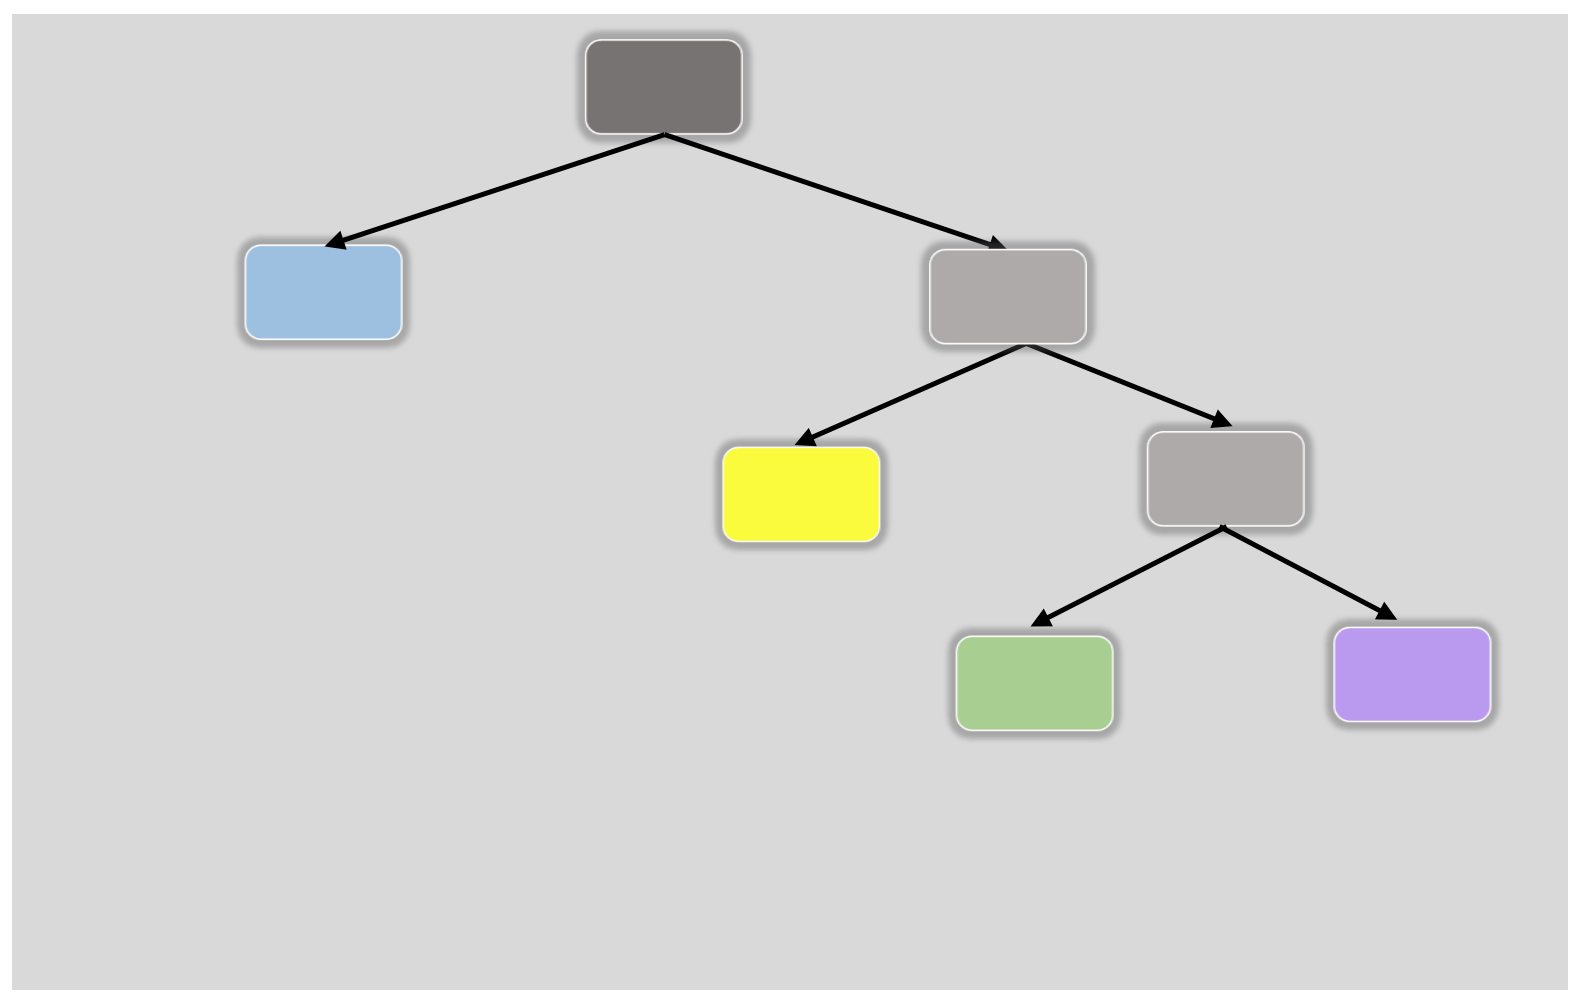
\includegraphics[scale=.4]{figs/T12_A.png}
%\end{center}
%}\\
%\end{frame}
%
%
%
%
%
%\begin{frame}
%\qBrd[4.7in]{babyblueeyes!50}{
%\begin{center}
%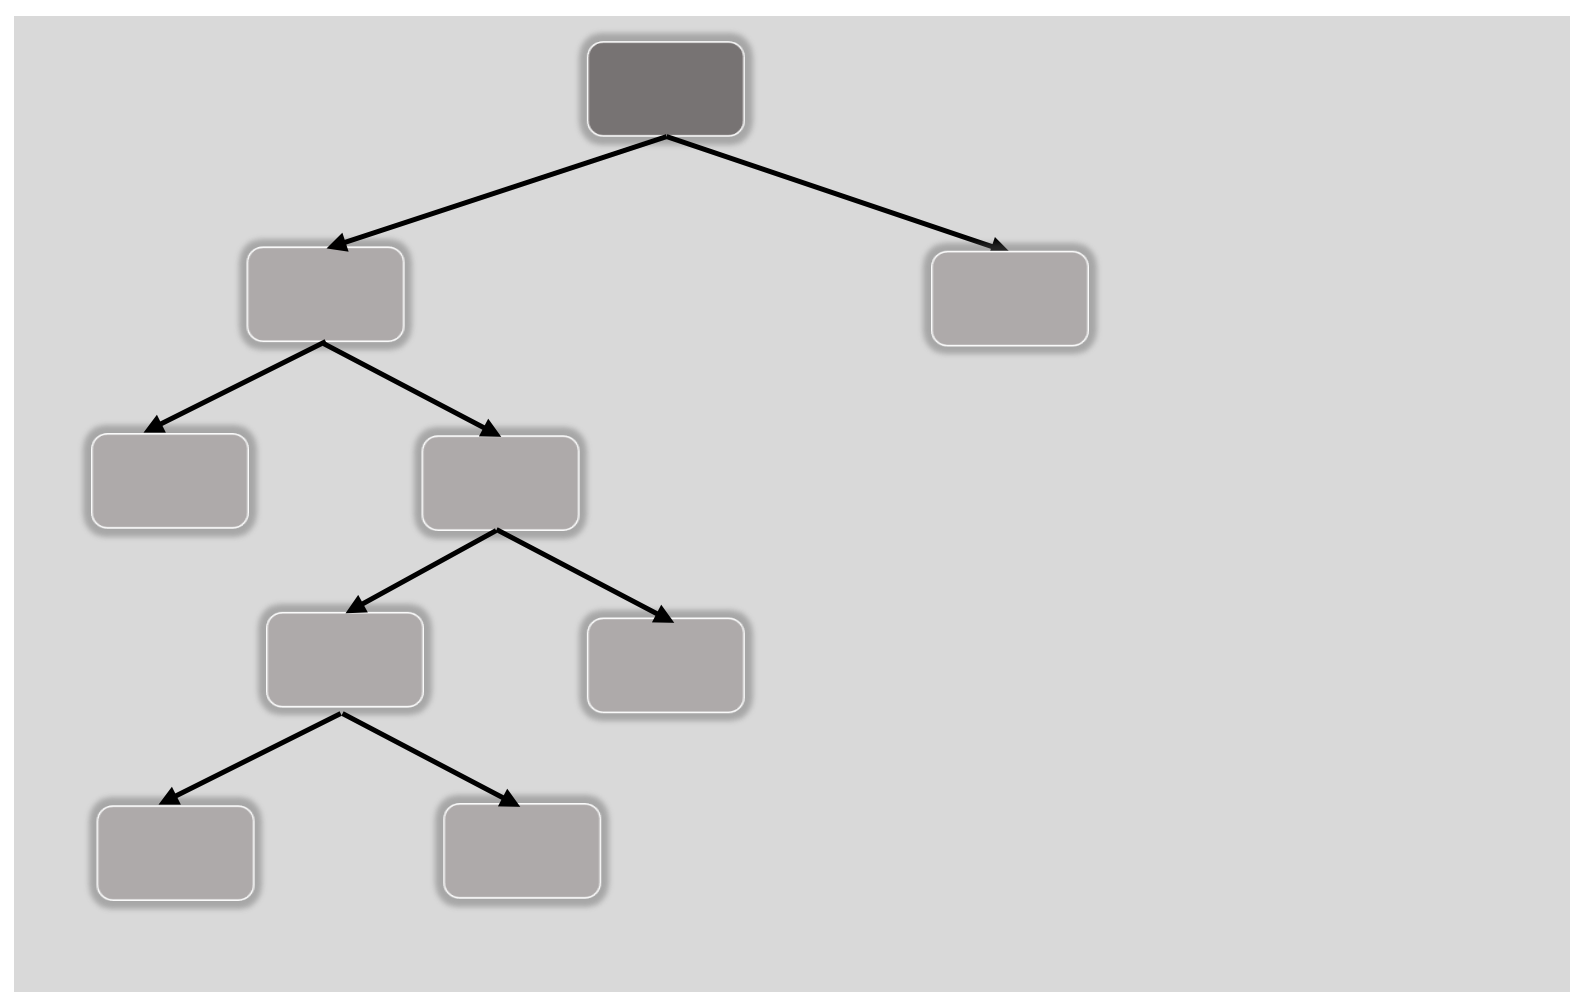
\includegraphics[scale=.4]{figs/T13_Q.png}
%\end{center}
%}\\
%\end{frame}
%
%
%\begin{frame}
%\qBrd[4.7in]{babyblueeyes!50}{
%\begin{center}
%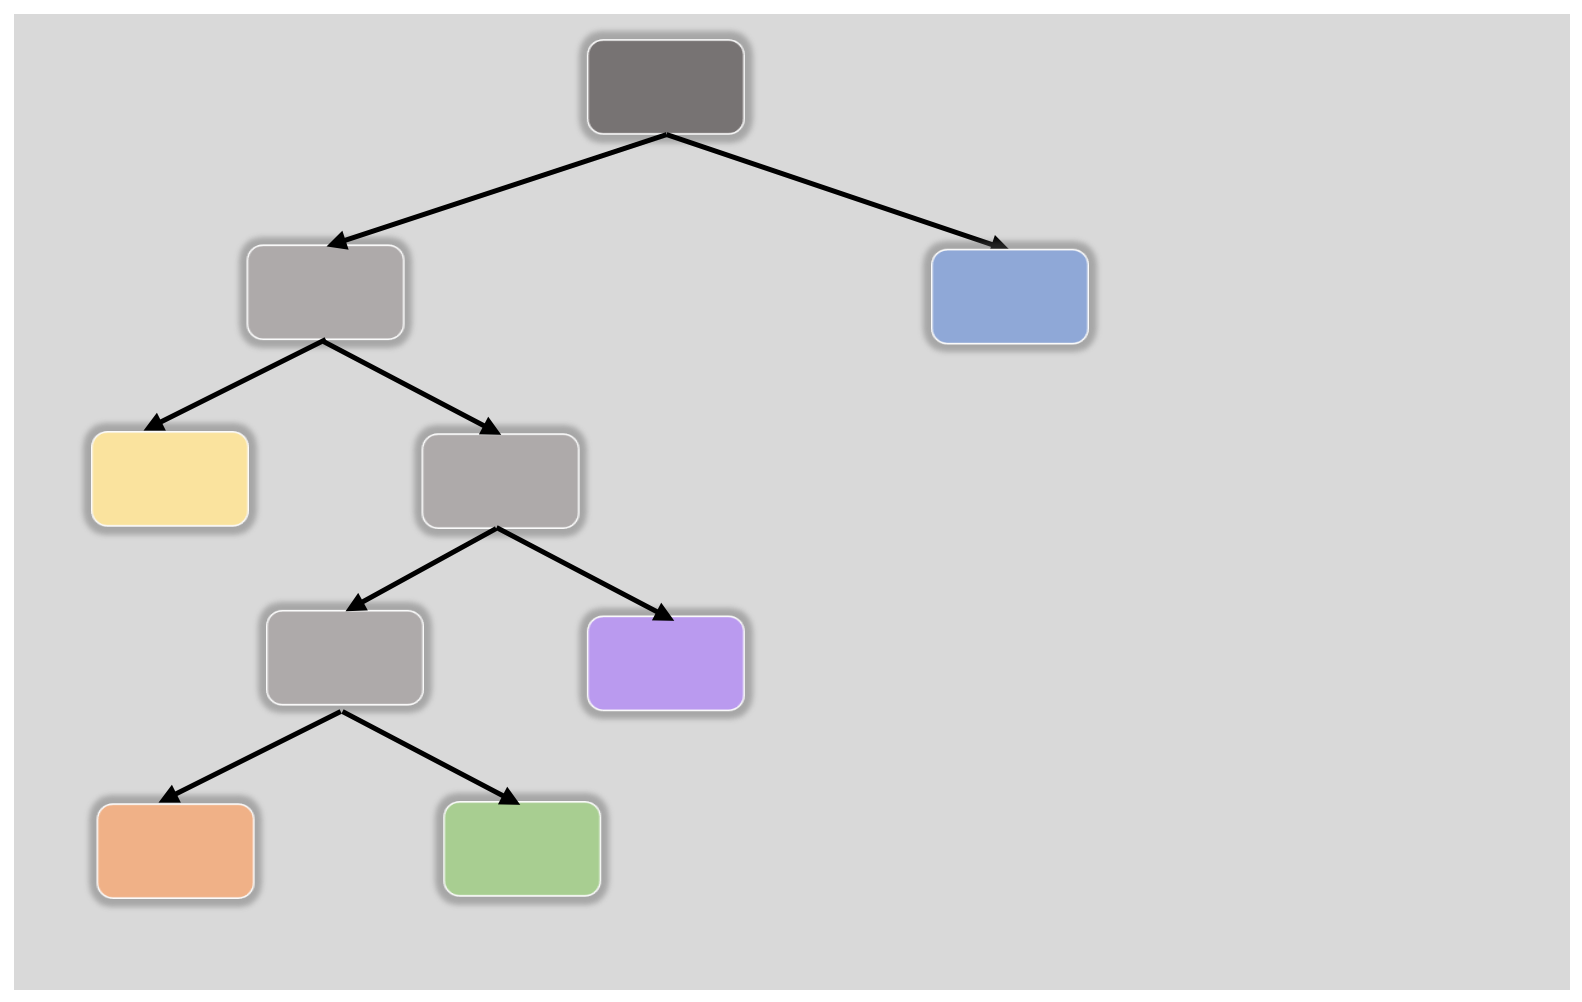
\includegraphics[scale=.4]{figs/T13_A.png}
%\end{center}
%}\\
%\end{frame}
%
%
%
%\begin{frame}
%\qBrd[4.7in]{babyblueeyes!50}{
%\begin{center}
%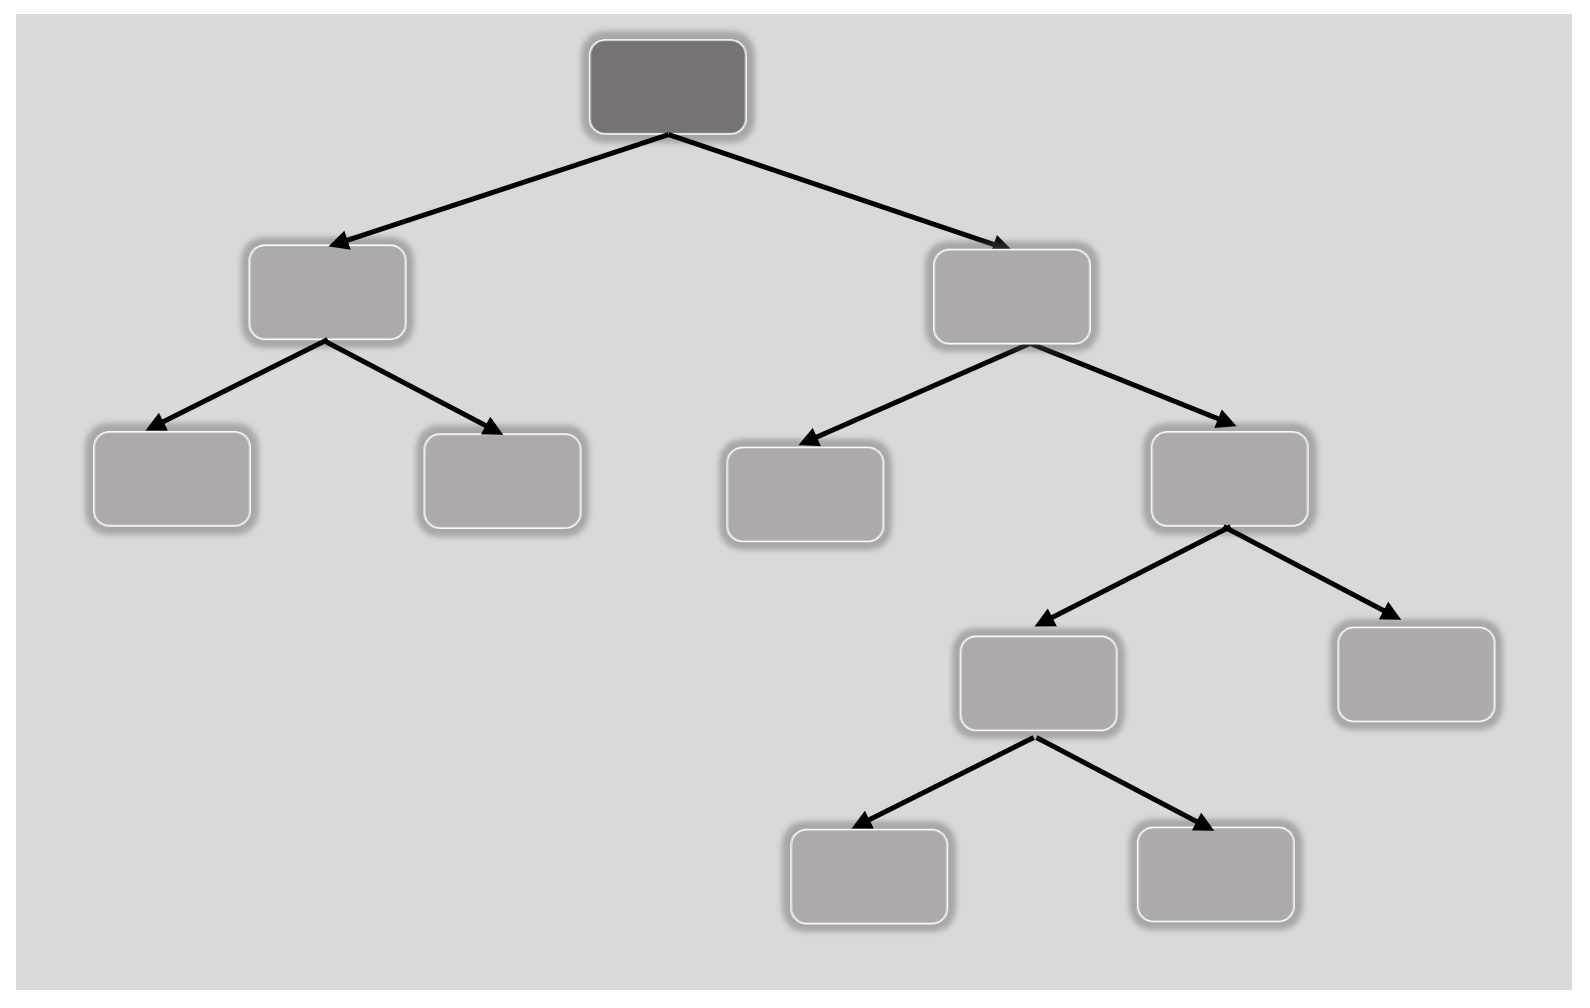
\includegraphics[scale=.4]{figs/T14_Q.png}
%\end{center}
%}\\
%\end{frame}
%
%
%\begin{frame}
%\qBrd[4.7in]{babyblueeyes!50}{
%\begin{center}
%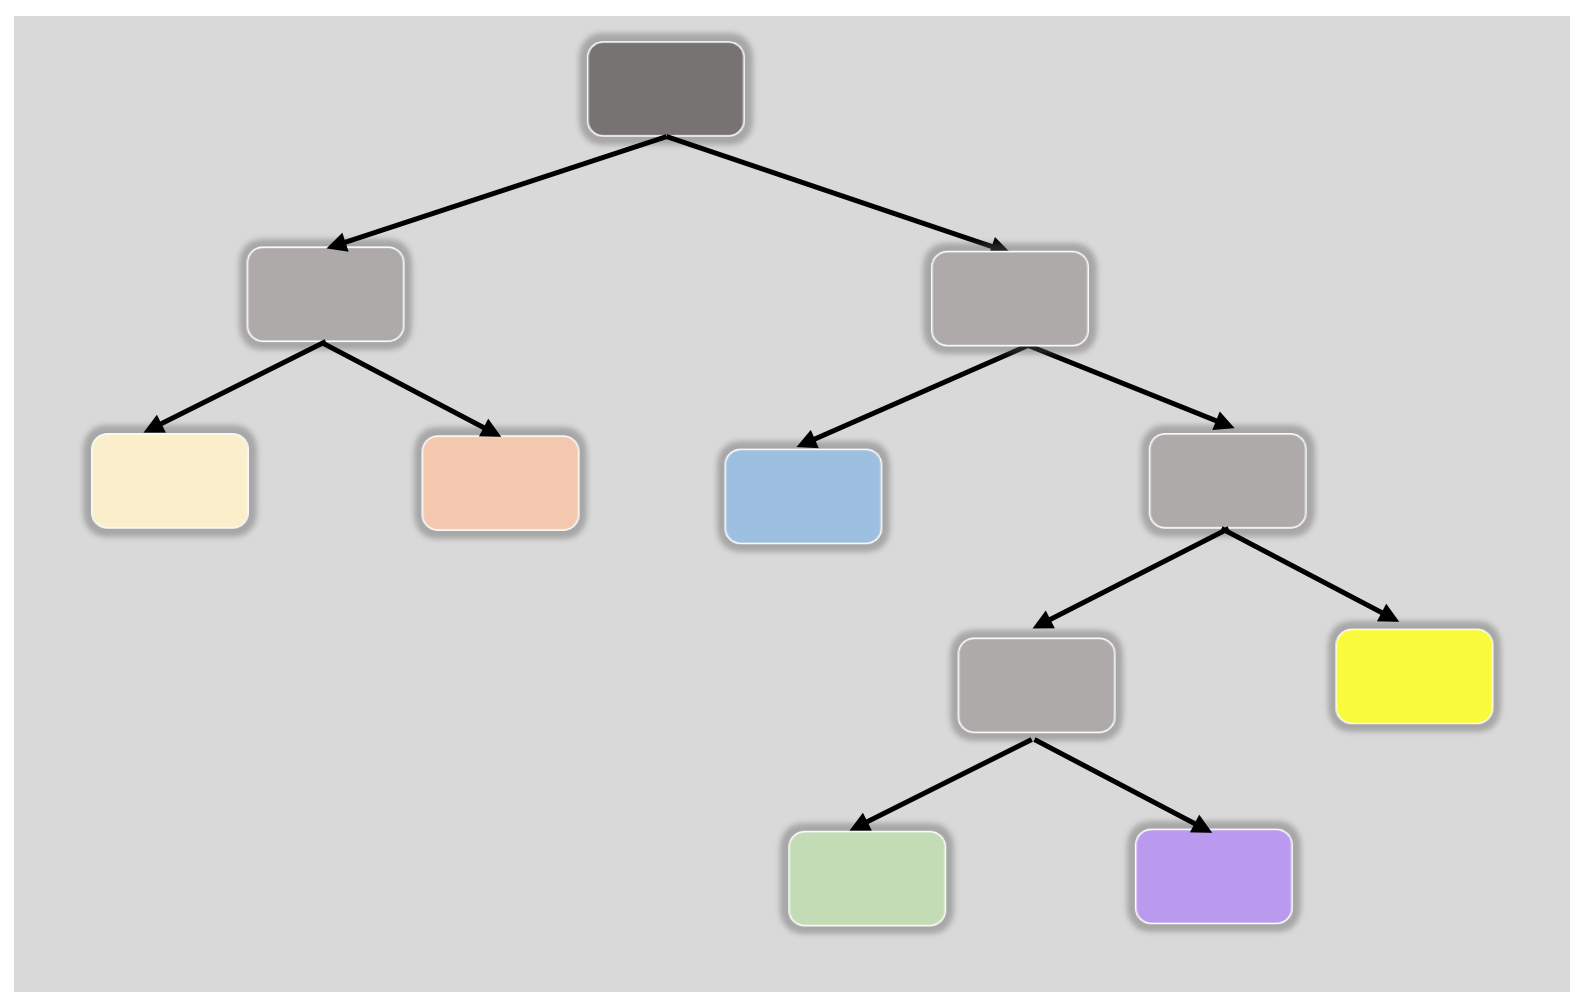
\includegraphics[scale=.4]{figs/T14_A.png}
%\end{center}
%}\\
%\end{frame}
%
%
%
%
%\TransitionFrame[antiquebrass]{\Large  Tree Pruning }
%%
%
%
%
%\begin{frame}
%\qBrd[4.1in]{babyblueeyes!60}{ $$\HLTW{ \displaystyle
%\mathcal{C}ost(T):}=   \DBX{\HLTW{ \displaystyle \sum_{j=1}^{\vert T \vert } \sum_{i\in \HLTEQ[rose!40]{\HLTY{ R_j}}}^{}\left(y_i - \HLTY{ \widehat{c}_j} \right)^2  } +\HLTW{\alpha \vert  T \vert}} \text{ where } \DBX{ \HLTY{ \displaystyle  \widehat{c}_j}  =  \frac{\sum_{i \in R_j } y_i }{n_j}    }$$}\\
%
% \begin{center}
% 
% \qBrd[2.5in]{olive!60}{ 
% \begin{center}
% $\DBX{  \displaystyle T_{\alpha, {_\text{opt}}} = \argmin_{T \subseteq T_0 } \HLTW{\mathcal{C}ost(T)}}$
%  \end{center}
% }
% \end{center}
% 
% 
%
%\end{frame}




\TransitionFrame[antiquebrass]{\Large Thank You }

\end{document}
